%%% File encoding: UTF-8
%%% äöüÄÖÜß  <-- keine deutschen Umlaute hier? UTF-faehigen Editor verwenden!

%%% Magic Comments zum Setzen der korrekten Parameter in kompatiblen IDEs
% !TeX encoding = utf8
% !TeX program = pdflatex 
% !TeX spellcheck = de_DE
% !BIB program = biber

\documentclass[master,german]{hgbthesis}
% Zulässige Optionen in [..]: 
%   Typ der Arbeit: diploma, master (default), bachelor, internship 
%   Hauptsprache: german (default), english
%%%----------------------------------------------------------

\RequirePackage[utf8]{inputenc}		% bei der Verw. von lualatex oder xelatex entfernen!

\graphicspath{{images/}}    % Verzeichnis mit Bildern und Grafiken
\logofile{logo}				% Logo-Datei = images/logo.pdf (\logofile{}, wenn kein Logo gewünscht)
\bibliography{references}  	% Biblatex-Literaturdatei (references.bib)

%%%----------------------------------------------------------
% Angaben für die Titelei (Titelseite, Erklärung etc.)
%%%----------------------------------------------------------

%%% Einträge für ALLE Arbeiten: -----------------------------
\title{Partielle Lösungen zur allgemeinen Problematik}
\author{Peter A.\ Schlaumeier}
\programname{Universal Computing}
\placeofstudy{Hagenberg}
\dateofsubmission{2018}{07}{10}	% {YYYY}{MM}{DD}

%%% Zusätzlich für eine Bachelorarbeit: ---------------------
\thesisnumber{XXXXXXXXXX-A}   % Stud-ID, z.B. 1310238045-A  
% (A = 1. Bachelorarbeit)
\semester{Sommersemester 2016} 
\coursetitle{Einführung in die Tiefere Problematik 1} 
\advisor{Alois B.~Treuer, Päd.\ Phil.}

%%% Restriktive Lizenformel anstatt CC (nur für Typ master) -
%\strictlicense

%%%----------------------------------------------------------
\begin{document}
%%%----------------------------------------------------------

%%%----------------------------------------------------------
\frontmatter                    % Titelei (röm. Seitenzahlen)
%%%----------------------------------------------------------

\maketitle
\tableofcontents

\chapter{Vorwort} 	% engl. Preface


Dies ist \textbf{Version \hgbDate} der \latex-Dokumentenvorlage für 
verschiedene Abschlussarbeiten an der Fakultät für Informatik, Kommunikation
und Medien der FH Oberösterreich in Hagenberg, die mittlerweile auch 
an anderen Hochschulen im In- und Ausland gerne verwendet wird.

Das Dokument entstand ursprünglich auf Anfragen von Studierenden,
nachdem im Studienjahr 2000/01 erstmals ein offizieller
\latex-Grundkurs im Studiengang Medientechnik und -design an der
FH Hagenberg angeboten wurde. Eigentlich war die Idee, die bereits
bestehende \emph{Word}-Vorlage für Diplomarbeiten "`einfach"' in
\latex\ zu übersetzen und dazu eventuell einige spezielle
Ergänzungen einzubauen. Das erwies sich rasch als wenig
zielführend, da \latex, \va was den Umgang mit Literatur und
Grafiken anbelangt, doch eine wesentlich andere Arbeitsweise
verlangt. Das Ergebnis ist -- von Grund auf neu geschrieben und
wesentlich umfangreicher als das vorherige Dokument --
letztendlich eine Anleitung für das Schreiben mit \latex, ergänzt
mit einigen speziellen (mittlerweile entfernten) Hinweisen für \emph{Word}-Benutzer.
Technische Details zur aktuellen Version finden sich in Anhang \ref{app:TechnischeInfos}.

Während dieses Dokument anfangs ausschließlich für die Erstellung
von Diplomarbeiten gedacht war, sind nunmehr auch  
\emph{Masterarbeiten}, \emph{Bachelor\-arbeiten} und \emph{Praktikumsberichte} 
abgedeckt, wobei die Unterschiede bewusst gering gehalten wurden.

Bei der Zusammenstellung dieser Vorlage wurde versucht, mit der
Basisfunktionalität von \latex das Auslangen zu finden und -- soweit möglich --
auf zusätzliche Pakete zu verzichten. Das ist nur zum Teil gelungen;
tat\-säch\-lich ist eine Reihe von ergänzenden "`Paketen"' notwendig, wobei jedoch
nur auf gängige Erweiterungen zurückgegriffen wurde.
Selbstverständlich gibt es darüber hinaus eine Vielzahl weiterer Pakete,
die für weitere Verbesserungen und Finessen nützlich sein können. Damit kann
sich aber jeder selbst beschäftigen, sobald das notwendige Selbstvertrauen und
genügend Zeit zum Experimentieren vorhanden sind.
Eine Vielzahl von Details und Tricks sind zwar in diesem Dokument nicht explizit
angeführt, können aber im zugehörigen Quelltext jederzeit ausgeforscht
werden.

Zahlreiche KollegInnen haben durch sorgfältiges Korrekturlesen und
konstruktive Verbesserungsvorschläge wertvolle Unterstützung
geliefert. Speziell bedanken möchte ich mich bei Heinz Dobler für
die konsequente Verbesserung meines "`Computer Slangs"', bei
Elisabeth Mitterbauer für das bewährte orthographische Auge und
bei Wolfgang Hochleitner für die Tests unter Mac~OS.

Die Verwendung dieser Vorlage ist jedermann freigestellt und an
keinerlei Erwähnung gebunden. Allerdings -- wer sie als Grundlage
seiner eigenen Arbeit verwenden möchte, sollte nicht einfach
("`ung'schaut"') darauf los werken, sondern zumindest die
wichtigsten Teile des Dokuments \emph{lesen} und nach Möglichkeit
auch beherzigen. Die Erfahrung zeigt, dass dies die Qualität der
Ergebnisse deutlich zu steigern vermag.

Dieses Dokument und die zugehörigen \latex-Klassen sind seit Nov.\ 2017 auf CTAN%
\footnote{Comprehensive TeX Archive Network} 
als Paket \texttt{hagenberg-thesis} verfügbar unter
%
\begin{itemize}
\item[]\url{https://ctan.org/pkg/hagenberg-thesis}.
\end{itemize}
%
Den jeweils aktuellen Quelltexte sowie zusätzliche Materialien findet man unter
%
\begin{itemize}
\item[]\url{https://github.com/Digital-Media/HagenbergThesis}.%
\footnote{Unter \url{https://github.com/Digital-Media/HagenbergThesis/commits/master} 
findet man auch eine (früher im Anhang dieses Dokuments enthaltene) chronologische Auflistung der 
Änderungen.}
\end{itemize}



\noindent
Trotz großer Mühe enthält ein Dokument wie dieses immer Fehler und Unzulänglichkeiten
-- Kommentare, Verbesserungsvorschläge und sinnvolle Ergänzungen
sind daher willkommen, am einfachsten als Kommentar oder Fehlermeldung ("`Issue"') 
auf GitHub oder jederzeit auch per E-Mail an
%
\begin{itemize}
\item[]
Dr.\ Wilhelm Burger, Department für Digitale Medien,\newline
Fachhochschule Oberösterreich, Campus Hagenberg (Österreich)\newline
\nolinkurl{wilhelm.burger@fh-hagenberg.at}
\end{itemize}

\noindent
Übrigens, hier im Vorwort (das bei Diplom- und Masterarbeiten üblich, bei Bachelorarbeiten 
aber entbehrlich ist) kann kurz auf die Entstehung des Dokuments eingegangen werden.
Hier ist auch der Platz für allfällige Danksagungen (\zB an den Betreuer, 
den Begutachter, die Familie, den Hund, \ldots), Widmungen und philosophische 
Anmerkungen. Das sollte man allerdings auch nicht übertreiben und auf 
einen Umfang von maximal zwei Seiten beschränken.




 % Optional. Ggf. weglassen
\chapter{Kurzfassung}

An dieser Stelle steht eine Zusammenfassung der Arbeit, Umfang
max.\ 1 Seite. Im Unterschied zu anderen Kapiteln ist die
Kurzfassung (und das Abstract) üblicherweise nicht in Abschnitte
und Unterabschnitte gegliedert. 
Auch Fußnoten sind hier falsch am Platz.

Kurzfassungen werden übrigens häufig -- zusammen mit Autor und Titel
der Arbeit -- %
in Literaturdatenbanken aufgenommen. Es ist daher darauf zu
achten, dass die Information in der Kurzfassung für sich 
\emph{allein} (\dah ohne weitere Teile der Arbeit) zusammenhängend und
abgeschlossen ist. Insbesondere werden an dieser Stelle (wie \ua
auch im \emph{Titel} der Arbeit und im \emph{Abstract})
normalerweise \emph{keine Literaturverweise} verwendet! Falls
unbedingt solche benötigt werden -- etwa weil die Arbeit eine
Weiterentwicklung einer bestimmten, früheren Arbeit darstellt --,
dann sind \emph{vollständige} Quellenangaben in der Kurzfassung
selbst notwendig, \zB %
[\textsc{Zobel} J.: \textit{Writing for Computer Science -- The Art of
Effective Commu\-nica\-tion}. Springer-Verlag, Singa\-pur, 1997].

Auch sollte daran gedacht werden, dass bei der Aufnahme in Datenbanken
Sonderzeichen oder etwa Aufzählungen mit "`Knödellisten"' in der
Regel verloren gehen. Dasselbe gilt natürlich auch für das 
\emph{Abstract}.


Inhaltlich sollte die Kurzfassung \emph{keine} Auflistung der
einzelnen Kapitel sein (dafür ist das Einleitungskapitel
vorgesehen), sondern dem Leser einen kompakten, inhaltlichen
Überblick über die gesamte Arbeit verschaffen. Der hier verwendete
Aufbau ist daher zwangsläufig anders als der in der Einleitung.
		
\chapter{Abstract}


This should be a 1-page (maximum) summary of your work in English.

			

%%%----------------------------------------------------------
\mainmatter          % Hauptteil (ab hier arab. Seitenzahlen)
%%%----------------------------------------------------------

\chapter{Einleitung}
\label{cha:Einleitung}

\section{Zielsetzung}
Dieses Dokument ist als vorwiegend technische Starthilfe für das
Erstellen einer Masterarbeit (oder Bachelorarbeit) mit \latex
gedacht und ist die Weiterentwicklung einer früheren
Vorlage\footnote{Nicht mehr verfügbar.} für das Arbeiten mit
Microsoft \emph{Word}. Während ursprünglich daran gedacht war, die
bestehende Vorlage einfach in \latex zu übernehmen, wurde rasch
klar, dass allein aufgrund der großen Unterschiede zum Arbeiten
mit \emph{Word} ein gänzlich anderer Ansatz notwendig wurde. Dazu
kamen zahlreiche Erfahrungen mit Diplomarbeiten in den
nachfolgenden Jahren, die zu einigen zusätzlichen Hinweisen Anlass gaben.

Das vorliegende Dokument dient einem zweifachen Zweck: 
\emph{erstens} als Erläuterung und Anleitung, \emph{zweitens} als
direkter Ausgangspunkt für die eigene Arbeit. Angenommen wird,
dass der Leser bereits über elementare Kenntnisse im Umgang mit
\latex verfügt. In diesem Fall sollte -- eine einwandfreie
Installation der Software vorausgesetzt -- der Arbeit nichts mehr
im Wege stehen. Auch sonst ist der Start mit \latex\ nicht
schwierig, da viele hilfreiche Informationen auf den zugehörigen
Webseiten zu finden sind (s.\ Kap.~\ref{cha:ArbeitenMitLatex}).





\section{Warum {\latex}?}

Diplomarbeiten, Dissertationen und Bücher im
technisch-natur\-wissen\-schaft\-lichen Bereich werden
traditionell mithilfe des Textverarbeitungssystems \latex
\cite{Lamport1994, Lamport1995} gesetzt. Das hat gute Gründe, denn
\latex ist bzgl.\ der Qualität des Druckbilds, des Umgangs mit
mathematischen Elementen, Literaturverzeichnissen etc.\
unübertroffen und ist noch dazu frei verfügbar. Wer mit \latex
bereits vertraut ist, sollte es auch für die Abschlussarbeit
unbedingt in Betracht ziehen, aber auch für den Anfänger sollte
sich die zusätzliche Mühe am Ende durchaus lohnen.

Für den professionellen elektronischen Buchsatz wurde früher
häufig \emph{Adobe Framemaker} verwendet, allerdings ist diese
Software teuer und komplex. Eine modernere Alternative dazu ist
\emph{Adobe InDesign}, wobei allerdings die Erstellung
mathematischer Elemente und die Verwaltung von Literaturverweisen
zur Zeit nur rudimentär unterstützt werden.%
\footnote{Angeblich werden aber für den (sehr sauberen) Schriftsatz 
in \emph{InDesign} ähnliche Algorithmen wie in \latex\ verwendet.}

Microsoft \emph{Word} gilt im Unterschied zu \latex, 
\emph{Framemaker} und \emph{InDesign} übrigens nicht als professionelle
Textverarbeitungssoftware, obwohl es immer häufiger auch von
großen Verlagen verwendet wird.%
\footnote{Siehe auch \url{http://latex.tugraz.at/mythen.php}.}
Das Schriftbild in \emph{Word}
lässt -- zumindest für das geschulte Auge -- einiges zu wünschen
übrig und das Erstellen von Büchern und ähnlich großen Dokumenten
wird nur unzureichend unterstützt. Allerdings ist \emph{Word} sehr
verbreitet, flexibel und vielen Benutzern zumindest oberflächlich
vertraut, sodass das Erlernen eines speziellen Werkzeugs wie
\latex\ ausschließlich für das Erstellen einer Abschlussarbeit
manchen verständlicherweise zu mühevoll ist. Es sollte daher
niemandem übel genommen werden, wenn er/sie sich auch bei der Abschlussarbeit
auf \emph{Word} verlässt. Im Endeffekt lässt sich mit etwas
Sorgfalt (und ein paar Tricks) auch damit ein durchaus akzeptables
Ergebnis erzielen. 
Ansonsten sollten auch für \emph{Word}-Benutzer 
einige Teile dieses Dokuments von Interesse sein, insbesondere die
Abschnitte über Abbildungen und Tabellen
(Kap.~\ref{cha:Abbildungen}) und mathematische Elemente
(Kap.~\ref{cha:Mathematik}).


\section{Aufbau der Arbeit}

Hier am Ende des Einleitungskapitels (und nicht
etwa in der Kurzfassung) ist der richtige Platz, um die
inhaltliche Gliederung der nachfolgenden Arbeit zu beschreiben.
Hier sollte man darstellen, welche Teile (Kapitel) der Arbeit
welche Funktion haben und wie sie inhaltlich zusammenhängen. Auch
die Inhalte des \emph{Anhangs} -- sofern vorgesehen -- sollten hier
kurz beschrieben werden.

Zunächst sind in Kapitel \ref{cha:Abschlussarbeit} einige wichtige
Punkte zu Abschlussarbeiten im Allgemeinen zusammengefasst.
Kapitel \ref{cha:ArbeitenMitLatex} beschreibt die Idee und die
grundlegenden technischen Eigenschaften von \latex.
Kapitel \ref{cha:Abbildungen} widmet sich der Erstellung von Abbildungen
und Tabellen sowie der Einbindung von Quellcode.
Mathematische Elemente und Gleichungen sind das Thema in Kapitel \ref{cha:Mathematik} 
\usw
Anhang \ref{app:TechnischeInfos} enthält technische Details zu
dieser Vorlage, 
Anhang \ref{app:materials} enthält eine Auflistung von zugehörigen Materialien
auf einem beigelegten Speichermedium, und 
Anhang \ref{app:Fragebogen} zeigt ein Beispiel für die
Einbindung eines mehrseitigen PDF-Dokuments.







\chapter{Die Abschlussarbeit}
\label{cha:Abschlussarbeit}

Jede Abschlussarbeit%
\footnote{Die meisten der folgenden Bemerkungen gelten gleichsam für Bachelor-, Master- und Diplomarbeiten.} 
ist anders und dennoch sind sich gute
Arbeiten in ihrer Struktur meist sehr ähnlich, \va\ bei
technisch-natur\-wissen\-schaft\-lichen Themen. 

\section{Elemente der Abschlussarbeit}

Als Ausgangspunkt bewährt hat sich der folgende Grundaufbau, der natürlich 
vari\-iert und beliebig verfeinert werden kann:
%
\begin{enumerate}
\item \textbf{Einführung und Motivation}: Was ist die Problem- oder Aufgabenstellung und
warum sollte sich jemand dafür interessieren?
\item \textbf{Präzisierung des Themas}: Hier wird der aktuelle Stand der Technik
oder Wissenschaft ("`State-Of-The-Art"') beschrieben, es werden bestehende
Defizite oder offene Fragen aufgezeigt und daraus die
Stoßrichtung der eigenen Arbeit entwickelt.
\item \textbf{Eigener Ansatz}: Das ist natürlich der Kern der Arbeit. Hier
wird gezeigt, wie die vorher beschriebene Aufgabenstellung gelöst und --
häufig in Form eines Programms%
\footnote{\emph{Prototyp} ist in diesem Zusammenhang ein gerne benutzter Begriff, der im Deutschen
allerdings oft unrichtig dekliniert wird. Richtig ist: der \emph{Prototyp}, des \emph{Prototyps}, dem/den \emph{Protototyp} -- falsch hingegen \zB: des \emph{Prototyp\underline{en}}!
} --
realisiert wird, ergänzt durch illustrative Beispiele.
\item \textbf{Zusammenfassung}: Was wurde erreicht und welche Ziele sind
noch offen geblieben, wo könnte weiter gearbeitet werden?
\end{enumerate}
%
Natürlich ist auch ein gewisser dramaturgischer Aufbau der Arbeit
wichtig, wobei zu bedenken ist, dass der Leser in der Regel nur
wenig Zeit hat und -- anders als etwa bei einem Roman -- seine
Geduld nicht auf die lange Folter gespannt werden darf. Erklären
Sie bereits in der Einführung (und nicht erst im letzten Kapitel),
wie Sie an die Sache herangehen, welche Lösungen Sie vorschlagen
und wie erfolgreich Sie damit waren.

Übrigens, auch Fehler und Sackgassen dürfen (und sollten)
beschrieben werden; ihre Kenntnis hilft oft doppelte Experimente und
weitere Fehler zu vermeiden und ist damit sicher nützlicher als
jede Schönfärberei.
Und natürlich ist es auch nicht verboten, seine eigene Meinung 
in sachlicher Form zu äußern.


\section{Arbeiten in Englisch}
\label{sec:englisch}

Diese Vorlage ist zunächst darauf abgestellt, dass die
Abschlussarbeit in deutscher Sprache erstellt wird. Vor allem bei
Arbeiten, die in Zusammenarbeit mit größeren Firmen oder
internationalen Instituten entstehen, ist es häufig erwünscht,
dass die Abschlussarbeit zu besseren Nutzbarkeit in englischer
Sprache verfasst wird, und viele Hochschulen%
\footnote{Die FH Oberösterreich macht hier keine Ausnahme. 
Der Begriff "`Fachhochschule"' wird dabei entweder gar nicht
übersetzt oder -- wie im deutschsprachigen Raum mittlerweile üblich -- 
mit \emph{University of Applied Sciences}.
%Die offizielle englische Übersetzung von "`Medientechnik und -design"'
%ist übrigens \emph{Media Technology and Design}.
} 
lassen dies in
der Regel auch zu.

Beachtet sollte allerdings werden, dass das Schreiben dadurch nicht
einfacher wird, auch wenn einem Worte und Sätze im Englischen
scheinbar leichter "`aus der Feder"' fließen. Gerade im Bereich
der Informatik erscheint durch die Dominanz englischer
Fachausdrücke das Schreiben im Deutschen mühsam und das Ausweichen
ins Englische daher besonders attraktiv. Das ist jedoch
trügerisch, da die eigene Fertigkeit in der Fremdsprache
(trotz der meist langjährigen Schulbildung) häufig überschätzt wird.
Prägnanz und Klarheit gehen leicht verloren und bisweilen ist das
Resultat ein peinliches Gefasel ohne Zusammenhang und soliden
Inhalt. Sofern die eigenen Englischkenntnisse nicht wirklich gut sind, ist
es ratsam, zumindest die wichtigsten Teile der Arbeit zunächst in
Deutsch zu verfassen und erst nachträglich zu übersetzen. Besondere Vorsicht ist bei der Übersetzung von scheinbar
vertrauten Fachausdrücken angebracht. Zusätzlich ist es immer zu
empfehlen, die fertige Arbeit von einem "`native speaker"'
korrigieren zu lassen.



Technisch ist, außer der Spracheinstellung und den
unterschiedlichen Anführungszeichen (s.\
Abschn.~\ref{sec:anfuehrungszeichen}), für eine englische Arbeit
nicht viel zu ändern, allerdings sollte Folgendes beachtet werden:
%
\begin{itemize}
\item  Die Titelseite (mit der Bezeichnung "`Diplomarbeit"' oder "`Masterarbeit"') 
ist für die einzureichenden Exemplare jedenfalls in \emph{deutsch} zu halten,
auch wenn der Titel englisch ist. 
\item Ebenso muss neben dem
englischen \emph{Abstract} auch eine deutsche \emph{Kurzfassung}
enthalten sein. %
\item Akademische Titel von Personen haben im Englischen offenbar
weniger Bedeutung als im Deutschen und werden daher meist
weggelassen.
\end{itemize}

\chapter{Zum Arbeiten mit \latex}
\label{cha:ArbeitenMitLatex}

\section{Einstieg}
\label{sec:LatexEinstieg}

\latex ist eine in den Naturwissenschaften sehr verbreitete
und mittlerweile klassische Textverarbeitungssoftware für das Erstellen
großer und komplizierter Dokumente mit professionellem Anspruch.
Das Arbeiten mit \latex erscheint -- zumindest für ungeübte Benutzer*innen -- %
zunächst schwieriger als mit herkömmlichen Werkzeugen für die
Textverarbeitung.

Zum Ersten ist -- im Unterschied zu den meisten gängigen
Text\-ver\-arbei\-tungs\-prog\-ram\-men -- \latex nicht \textsc{Wysiwyg}%
\footnote{"What You See Is What You Get." Es gibt auch 
\textsc{Wysiwyg}-Implementierungen für \latex, 
\zB\ \emph{Scientific WorkPlace} (\url{https://www.mackichan.com/}) oder
\emph{LyX} (\url{https://www.lyx.org/}), 
die aber teuer \bzw\ relativ langsam sind.},
sondern es handelt sich um eine \emph{Markup Lang\-uage} (wie HTML) -- noch dazu
eine für Anfänger*innen recht komplizierte -- und zugehörige Werkzeuge.
Ungewohnt erscheinen sicher auch die vermeintlich starken
Einschränkungen von \latex,
insbesondere in Bezug auf die Wahl der Schriften und das
Layout. Während anfangs of der Eindruck entsteht, dass diese Rigidität
die eigene Kreativität beschränkt, fällt mit der Zeit auf, dass es gerade
dadurch gelingt, sich stärker auf die Inhalte der Arbeit zu
konzentrieren als auf deren äußere Form. Dass am Ende die Form dennoch stimmt,
ist allerdings nur dann gewährleistet, wenn man sich bei den eigenen Modifikationen
der Formate und Parameter äußerste Zurückhaltung auferlegt, es sei denn,
man ist in der Zwischenzeit bereits selbst zum \latex-\emph{Guru} avanciert.

Insgesamt lohnt sich der Aufwand, wie viele meinen, zumal die Abschlussarbeit
in jedem Fall (mit oder ohne \latex) ein substantielles Stück Arbeit ist.
Allerdings sollte mithilfe von \latex ein professionell aussehendes
Ergebnis einfacher zu erreichen sein und es dürfte wohl auch einiger
Ärger mit Fehlern und Einschränkungen gängiger Software erspart bleiben.
Zudem könnte es durchaus sein, dass sich nebenbei auch das eigene Auge für
die Feinheiten des Buchsatzes (weiter-){\obnh}entwickelt.%
\footnote{Dieses abschließende Textelement wurde übrigens zur Ermöglichung eines 
Zeilenumbruchs nach der Klammer so gesetzt: \texttt{\ldots (weiter-)\{{\bs}optbreaknh\}entwickelt.}
Das Makro \texttt{{\bs}optbreaknh} ("optional break with no hyphen") ist in 
\texttt{hgb.sty} definiert.}


\subsection{Software}
\label{sec:Software}

Zum Arbeiten mit \latex wird -- neben einem Computer -- natürlich Software
benötigt. Mussten früher oft die einzelnen Komponenten von \latex mühevoll
zusammengesucht und für die eigene Umgebung konfiguriert werden, gibt es
mittlerweile für die wichtigsten Plattformen (Windows, Mac~Os, Linux) fertige
\latex-Installationen, die ohne weiteres Zutun laufen. Die aktuelle Version von
\latex\ ist \LaTeXe\ (sprich "LaTeX zwei e"). Zum lokalen Arbeiten mit \latex\
werden zwei Dinge benötigt:
%
\begin{itemize}
\item \latex-Installation (Distribution),
\item Texteditor oder Autor*innenumgebung (Frontend).
\end{itemize}
%
Sämtliche Komponenten sind kostenlos und für alle gängigen Plattformen verfügbar.

Alternativ kann auch ein Online-Editor verwendet werden, der ein Arbeiten im
Browser ermöglicht und keinerlei Installation auf dem eigenen Rechner
voraussetzt. Details zu empfohlenen Setups und möglichen Alternativen finden
sich in Anhang~\ref{app:TechnischeInfos}.


\subsection{Literatur}
\label{sec:literatur}

Es ist müßig, ohne geeignete Literatur mit \latex zu beginnen, selbst
fortgeschrittene Benutzer*innen werden immer wieder auf Hilfe angewiesen
sein. Erfreulicherweise ist sehr viel Nützliches auch online verfügbar.
Gute Startpunkte sind \zB
%
\begin{itemize}
\item \emph{\textrm{\LaTeXe}-Kurzbeschreibung} von Daniel et al.\ \cite{Daniel2018}
\item \emph{The Not So Short Introduction to \textrm{\LaTeXe}}
            von Oetiker et al.\ \cite{Oetiker2018}
\end{itemize}
%
\noindent
Als mittlerweile bereits klassisches Handbuch zu \latex ist
%
\begin{itemize}
  \item \emph{A Guide to \textrm{\LaTeX}} von H.~Kopka und P.~Daly \cite{Kopka2003}
\end{itemize}
%
zu empfehlen, zu dem es für Interessierte auch zwei vertiefende
Zusatzbände in Deutsch gibt. Zahlreiche weitere Dokumente zu
\latex und verwandten Themen finden sich \ua im Rahmen des {\em
Comprehensive TeX Archive Network} (CTAN) auf
\begin{quote}
	\url{https://www.ctan.org/}%
	\footnote{\url{https://www.ctan.org/topic/}}
\end{quote}
%
Besonders nützlich sind auch die
\emph{Comprehensive List of \textrm{\latex} Symbols} \cite{Pakin2020}
und die Beschreibungen wichtiger \latex-Pakete, wie
%
\begin{quote}
  \texttt{babel} \cite{Bezos2020},\newline
  \texttt{graphics}, \texttt{graphicx} \cite{Carlisle2020},\newline
  \texttt{fancyhdr} \cite{Oostrum2019},\newline
  \texttt{caption} \cite{Sommerfeldt2020}.
\end{quote}


\section{Schrift}

In einem \latex-Dokument muss zunächst die verwendete Schriftart festgelegt werden. Im Text können dann mittels diverser Auszeichnungen Textstellen durch eine Änderung des Schriftstils hervorgehoben werden.

\subsection{Schriftarten}

\latex verwendet normalerweise die Schriften der \emph{Computer
Modern}
(CM) Serie, die so wie die \emph{TeX}-Software selbst von Donald Knuth%
\footnote{\url{https://www-cs-faculty.stanford.edu/~knuth/}} entwickelt
wurden. Die drei Basis-Schrifttypen der CM-Serie in \latex sind
%
\begin{quote}
\begin{tabular}{lcl}
\textrm{Roman}      & & \verb!\textrm{Roman}!,\\
\textsf{Sans Serif} & & \verb!\textsf{Sans Serif}!,\\
\texttt{Typewriter} & & \verb!\texttt{Typewriter}!.\\
\end{tabular}
\end{quote}
%
\noindent In den Augen vieler Benutzer*innen ist allein die Qualität und
Zeitlosigkeit dieser Schriften ein Grund, \latex für seriöse
Zwecke zu verwenden. Ein weiterer Vorteil der \emph{TeX}-Schriften
ist, dass die unterschiedlichen Schriftfamilien und Schnitte
bezüglich der Größe sehr gut aufeinander abgestimmt sind.

Darüber hinaus können aber in \latex auch beliebige 
\emph{PostScript}-Schrif\-ten (Type 1) verwendet werden, was allerdings in
der Praxis einiges an "Tuning"-Arbeit verlangt. Häufig verwendet
werden \zB\ \emph{Times} und \emph{Palatino}, derzeit ist aber ein Trend 
zurück zu den klassischen CM-Schriften zu beobachten.



\subsection{Texte hervorheben}

Texte können auf unterschiedliche Weise aus dem Fließtext hervorgehoben werden.
\begin{itemize}
%
\item Die Auszeichnung in \textit{Kursivschrift} oder "italic" (\verb!\textit{..}!) ist \va\ zum Hervorheben von
Betonungen und Zitaten geeignet, aber auch für
Produktbezeichnungen, Fremdwörter und Variablen im Text, \zB
%
\begin{quote}
\verb!\textit{Variable}! $\rightarrow$ \textit{Variable}
\end{quote}
%
\item \textsl{Slanted} %
(\verb!\textsl{..}!) bedeutet eine geneigte Schrift und
unterscheidet sich damit deutlich von \textit{Italic}; 
zum Vergleich:
%
\begin{quote}
\verb!\textrm{Daimler-Chrysler}! $\rightarrow$ \textrm{Daimler-Chrysler} \newline%
\verb!\textsl{Daimler-Chrysler}! $\rightarrow$ \textsl{Daimler-Chrysler} \newline%
\verb!\textit{Daimler-Chrysler}! $\rightarrow$ \textit{Daimler-Chrysler}
\end{quote}
%
\item \textbf{Boldface} (\verb!\textbf{..}!) wird \ia\ verwendet für 
\textbf{Überschriften}, Bezeichnungen von \textbf{Abbildungen} und 
\textbf{Tabellen}, im Fließtext aber selten:
%
\begin{quote}
\verb!\textbf{Überschriften}! $\rightarrow$ \textbf{Überschriften}
\end{quote}
%
\item \emph{Emphasize} (\verb!\emph!) %
ist normalerweise gleichbedeutend mit \verb!\textit!, wobei
\verb!\emph! allerdings auch bei geschachtelten
Hervorhebungen und im Bereich anderer Schriftschnitte das
"Richtige" tut: 
%
\begin{quote}
\setlength{\tabcolsep}{0pt}%
\begin{tabular}{lcl}
\verb!\textrm{Du \emph{auch} hier?}! & $\;\rightarrow\;$ &
    \textrm{Du \emph{auch} hier?}
\\
\verb!\textit{Du \emph{auch} hier?}! & $\;\rightarrow\;$ &
    \textit{Du \emph{auch} hier?} 
\\
\verb!\textsl{Du \emph{auch} hier?}! & $\;\rightarrow\;$ & 
    \textsl{Du \emph{auch} hier?}
\\
\verb!\textbf{Du \emph{auch} hier?}! & $\;\rightarrow\;$ & 
    \textbf{Du \emph{auch} hier?}
\\
\verb!\texttt{Du \emph{auch} hier?}! & $\;\rightarrow\;$ & 
    \texttt{Du \emph{auch} hier?}
\end{tabular}
\end{quote}
%
\item \underline{Unterstreichungen} sind ein Relikt aus der 
Schreibmaschinenära und im modernen Schriftsatz
eigentlich \underline{überflüssig}. Sie sollten daher nur in
Ausnahmefällen verwendet werden, \zB
%
\begin{quote}
\verb!\underline{überflüssig}!%
\footnote{Unterstrichene Texte werden zudem nicht automatisch abgeteilt.}
\end{quote}
%
\end{itemize}



\section{Textstruktur}

Zur Strukturierung des eigenen Text stellt \latex eine Reihe von Auszeichnungen zur Verfügung.

\subsection{Absatztrennung}

Absätze werden in {\latex}-Quelltext ausschließlich durch das
Einfügen einer oder mehrerer \textbf{Leerzeilen} voneinander
getrennt, es sind also \emph{keinerlei sonstige Steueranweisungen}
notwendig!
%
\begin{center}
\setlength{\fboxrule}{0.2mm}
\setlength{\fboxsep}{2mm}
\fbox{%
\begin{minipage}{0.9\textwidth}
Besonders die Verwendung von \texttt{\textbackslash\textbackslash} und 
 \texttt{\textbackslash{newline}}
Anweisungen zur Absatztrennung ist ein häufig zu beobachtender \textbf{Fehler}. 
Vor normalen Absätzen auch \emph{nichts} verloren hat die
Anweisung \texttt{\textbackslash{paragraph}\{\}}
-- sie ist in \latex\ (im Unterschied zu HTML)
eine Markierung für Überschriften mit Titel (\su)!
\end{minipage}}
\end{center}

Üblicherweise wird von {\latex} zwischen aufeinanderfolgenden 
Ab\-sätzen \emph{kein} zusätzlicher vertikaler Abstand eingefügt.%
\footnote{Das ist die Standardeinstellung in {\latex} und
natürlich abhängig von der verwendeten Dokumentenklasse, Style
etc.} 
Allerdings wird die
\emph{erste} Zeile jedes Absatzes (mit Ausnahme des ersten Absatzes
eines Abschnitts) eingerückt, um so die Absatzgrenzen deutlich zu
machen. Dieses Schema hat sich nicht nur im traditionellen
Buchsatz bewährt%
\footnote{Wer es nicht glaubt, sollte sein Bücherregal (oder notfalls das seiner Eltern) nach Gegenbeispielen durchsuchen.}
und sollte auch beibehalten werden, es sei denn
es gibt wirklich \emph{sehr} gute Gründe dagegen.
Für alle übrigen Gliederungen im vertikalen Textfluss sind Überschriften (s.\ unten) vorgesehen.

% Note: as of 2017-06-12 the \SuperPar macro has been deactivated
%\SuperPar 
%Manchmal besteht allerdings der Wunsch, etwa zur Verdeutlichung eines inhaltlichen Sprungs \emph{zwischen} zwei Absätzen einen zusätzlichen Abstand einzufügen, ohne dabei eine neue Überschrift zu setzen. Das kann gegebenenfalls (wie vor dem aktuellen Absatz passiert) durch 
%%
%\begin{quote}
%\texttt{{\bs}SuperPar} \emph{Manchmal besteht allerdings der Wunsch, \ldots}
%\end{quote}
%%
%erreicht werden, sollte jedoch sehr sparsam und wirklich \textbf{nur in begründbaren Einzelfällen} verwendet werden.%
%\footnote{Das Makro \texttt{{\bs}SuperPar} ist in \texttt{hgb.sty} definiert.}




\subsection{Überschriften}
\label{sec:ueberschriften}

\latex\ bietet -- abhängig von der verwendeten Dokumentenklasse --
einen Satz vordefinierter Überschriftformate in folgender Ordnung:
%
\begin{quote}
\verb!\part{!\texttt{\em Titel}\verb!}!%
\footnote{\texttt{part} ist für die Gliederung eines
größeren Werks in mehrere Teile vorgesehen und wird üblicherweise
bei einer Abschlussarbeit (und auch in diesem Dokument) nicht
verwendet.}
\newline%
\verb!\chapter{!\texttt{\em Titel}\verb!}! \newline%
\verb!\section{!\texttt{\em Titel}\verb!}! \newline%
\verb!\subsection{!\texttt{\em Titel}\verb!}! \newline%
\verb!\subsubsection{!\texttt{\em Titel}\verb!}! \newline%
\verb!\paragraph{!\texttt{\em Titel}\verb!}! \newline%
\verb!\subparagraph{!\texttt{\em Titel}\verb!}!
\end{quote}
%

\paragraph{Häufiger Fehler:} Bei \verb!\paragraph{}! und
\verb!\subparagraph{}! läuft -- wie in diesem Absatz zu sehen --
der dem Titel folgende Text ohne Umbruch in der selben Zeile
weiter, weshalb im Titel auf eine passende Interpunktion (hier
\zB\ \underline{\texttt{:}}) geachtet werden sollte. Der horizontale Abstand
nach dem Titel allein würde diesen als Überschrift nicht erkennbar
machen.


\subsection{Listen}

Listen sind ein beliebtes Mittel zur Textstrukturierung. In
\latex\ sind -- ähnlich wie in HTML -- drei Arten von formatierten
Listen verfügbar: ungeordnete Auflistung ("Knödelliste"),
geordnete Auflistung (Aufzählung) und Beschreibungsliste
(Description):
%
\begin{verbatim}
    \begin{itemize}     ... \end{itemize}
    \begin{enumerate}   ... \end{enumerate}
    \begin{description} ... \end{description}
\end{verbatim}
%
Listeneinträge werden mit \verb!\item! markiert, bei \texttt{description}-Listen mit \verb!\item[!\texttt{\em titel}\verb!]!. Listen
können ineinander verschachtelt werden, wobei sich bei \texttt{itemize}- und \texttt{enumerate}-Listen die Aufzählungszeichen mit
der Schachtelungstiefe ändern (Details dazu in der
\latex-Dokumentation).


\subsection{Absatzformatierung und Zeilenabstand}

Abschlussarbeiten werden -- wie Bücher -- in der Regel einspaltig und
im Blocksatz formatiert, was für den Fließtext wegen der großen
Zeilenlänge vorteilhaft ist. Innerhalb von Tabellen kommt es
wegen der geringen Spaltenbreite jedoch häufig zu Problemen mit
Abteilungen und Blocksatz, weshalb dort ohne schlechtes
Gewissen zum Flattersatz ("ragged right") gegriffen werden sollte (wie
\zB\ in Tab.~\ref{tab:synthesis-techniques} auf Seite
\pageref{tab:synthesis-techniques}).


\subsection{Fußnoten}
Fußnoten können in \latex\ an beinahe jeder beliebigen Stelle,
jedenfalls aber in normalen Absätzen, durch die Anweisung
%
\begin{quote}
\verb!\footnote{!\texttt{\em Fußnotentext}\verb!}!
\end{quote}
%
gesetzt werden. Zwischen der \verb!\footnote!-Marke und dem davor
liegenden Text sollte grundsätzlich \emph{kein Leerzeichen} entstehen (eventuelle
Zeilen\-um\-brüche mit \verb!%! auskommentieren).
Die Nummerierung und Platzierung der Fußnoten
erfolgt automatisch, sehr große Fußnoten werden notfalls sogar auf
zwei aufeinanderfolgende Seiten umgebrochen.


\subsubsection{Fußnoten in Überschriften}

Auch das ist ab und zu nötig, ist aber \va\ deshalb kein so
einfacher Fall, weil die Fußnote in einer Überschrift nur an Ort
und Stelle aufscheinen darf, nicht aber im \emph{Inhaltsverzeichnis}! Ein
konkretes Beispiel dafür ist die Überschrift zu
Kapitel~\ref{cha:Schluss}, die folgendermaßen definiert ist:
%
\begin{quote}
\begin{verbatim}
\chapter[Schlussbemerkungen]%
        {Schlussbemerkungen%
        \protect\footnote{Diese Anmerkung ....}}%
\end{verbatim}
\end{quote}
%
Dabei ist der erste (optionale) Titel \verb![Schlussbemerkungen]!
der Eintrag im Inhaltsverzeichnis und im Seitenkopf. 
Der zweite (gleich lautende) Titel
\texttt{\{Schlussbemerkungen\}} erscheint auf der aktuellen Seite und
enthält auch den \verb!\footnote{}! Eintrag, der allerdings an
dieser Stelle durch die Direktive \verb!\protect! "geschützt"
werden muss. Die \verb!%!-Zeichen sind hier übrigens notwendig,
um eventuelle Leerzeichen, die durch Zeilenumbrüche im Quelltext
entstehen, zu eliminieren (dieser Trick wird 
in \latex\ häufig benötigt, s.\ Abschn.~\ref{sec:kommentare}). 
Ziemlich kompliziert also, und damit 
ein weiterer Grund, Fußnoten an solchen Stellen überhaupt zu vermeiden.

Generell sollte mit Fußnoten sparsam umgegangen werden, da sie den
Textfluss unterbrechen und den*die Leser*in ablenken. Insbesondere
sollten Fußnoten nicht (wie \va\ in manchen
sozialwissenschaftlichen Werken gepflegt) derart lang werden, dass
sie einen Großteil der Seite einnehmen und damit praktisch ein
zweites Dokument bilden.%
\footnote{Das führt bei Dokumenten mit vielen Fußnoten bei manchen
	Leser*innen angeblich so weit, dass sie aus Neugier (oder Versehen)
	regelmäßig bei den Fußnoten zu lesen beginnen und dann mühevoll die
	zugehörigen, kleingedruckten Verweise im Haupttext suchen.}


\subsection{Querverweise}
\label{sec:querverweise}

Zur Verwaltung von Querverweisen innerhalb eines Dokuments stellt
\latex\ einen sehr einfachen Mechanismus zur Verfügung. Zunächst
muss jede Stelle (Kapitel, Abschnitt, Abbildung, Tabelle etc.)
durch
%
\begin{quote}
\verb!\label{!\texttt{\em key}\verb!}!
\end{quote}
%
markiert werden, wobei \texttt{\em key} ein gültiges \latex-Symbol sein
muss. Damit Labels (die nur Zahlen sind) nicht verwechselt werden,
ist es üblich, sie je nach Bedeutung mit einer unterschiedlichen
Prefix zu versehen, \zB\
%
\begin{quote}
\tabcolsep0pt
\begin{tabular}{ll}
\verb!cha:!\texttt{\em kapitel}   & \ \ldots\ für Kapitel,  \\
\verb!sec:!\texttt{\em abschnitt} & \ \ldots\ für Abschnitte (Sections) und Unterabschnitte, \\
\verb!fig:!\texttt{\em abbildung} & \ \ldots\ für Abbildungen, \\
\verb!tab:!\texttt{\em tabelle}   & \ \ldots\ für Tabellen, \\
\verb!equ:!\texttt{\em gleichung} & \ \ldots\ für Formeln und Gleichungen.\\
\end{tabular}
\end{quote}
%
\noindent Beispiele:\ \verb!\label{cha:Einleitung}! oder
\verb!\label{fig:Screen-1}!. Mit den Anweisungen
%
\begin{quote}
\verb!\ref{!\texttt{\em key}\verb!}! 
\hspace{1em} oder \hspace{1em} 
\verb!\pageref{!\texttt{\em key}\verb!}!
\end{quote}
%
kann an beliebiger Stelle im Dokument die zu \texttt{\em key} gehörige
Nummer bzw.\ Seitennummer eingesetzt werden, \zB\
%
\begin{quote}
\verb!.. wie in Kap.~\ref{cha:Einleitung} erwähnt ..!\\
\verb!.. der Screenshot auf Seite \pageref{fig:Screen-1} ..!
\end{quote}
%
Übrigens werden die Bezeichnungen \emph{Kapitel} und {\em
Abschnitt} auffallend oft falsch verwendet -- Kapitel haben
ausschließlich "ungebrochene" Nummern:
%
\begin{quote}
\begin{tabular}{ll}
   \textrm{Richtig:\ } & Kapitel 7 oder Abschnitt 2.3.4\\
   \textbf{Falsch:\ }  & Kapitel 7.2 oder Abschnitt 5
\end{tabular}
\end{quote}


\section{Wortabstand und Interpunktion}

Während \latex in vielen Bereichen des Schriftsatzes automatisch das
bestmögliche Ergebnis zu erzielen versucht, ist bei der Interpunktion
Sorgfalt von Seiten des*der Autors*Autorin gefragt.

\subsection{\emph{French Spacing}}

Im englischsprachigen Schriftsatz ist es üblich, nach jedem
Satzende einen gegenüber dem normalen Wortzwischenraum
vergrößerten Abstand einzusetzen. Obwohl dies im Deutschen und
Französischen traditionell nicht so ist, wird es wegen der
verbesserten Lesbarkeit auch hier manchmal verwendet (nicht in diesem
Dokument). Falls die englische ("nicht-französische") Satztrennung mit
zusätzlichem Abstand bevorzugt wird, ist lediglich die Zeile
%
\begin{quote}
\verb!\nonfrenchspacing!
\end{quote}
%
am Beginn des Dokuments einzusetzen. 
In diesem Fall sollte 
aber die Interpunktion innerhalb von
Sätzen (nach .\ und :) sorgfältig beachtet weren. Beispielsweise
schreibt sich "Dr.\ Mabuse" in der Form
%
\begin{quote}
\verb!Dr.\ Mabuse! oder \verb!Dr.~Mabuse!
\end{quote}
%
Im zweiten Beispiel wird mit dem \verb!~! Zeichen zudem ein Zeilenumbruch am Leerzeichen verhindert.


\subsection{Gedanken- und Bindestriche}
\label{sec:gedankenstrich}

Die Verwendung der falschen Strichlängen (mit und ohne
Zwischenraum) ist ganz allgemein eine häufige Fehlerquelle.
Bewusst unterschieden werden sollte zwischen
%
\begin{itemize}
\item kurzen Bindestrichen (wie in "Wagner-Jauregg"), %
\item Minus-Zeichen, \zB\ $-7$ (erzeugt mit \verb!$-7$!), und %
\item echten Gedankenstrichen -- wie hier (erzeugt mit \verb!--!).
\end{itemize}
%
\noindent Für das Setzen von Gedankenstrichen\footnote{Für alle
drei gibt es übrigens auch in \emph{Word} entsprechende
Sonderzeichen.} gibt es eindeutige Konventionen:
%
\begin{enumerate}
\item Im \emph{Deutschen} wird üblicherweise einer von zwei
Leerzeichen umgebener Gedankenstrich%
\footnote{Halbgeviertstrich (\emph{En Dash}).} -- wie hier (in
\latex\ mit {\verb*! -- !}) gesetzt. Dieser wird auch für die Angabe von
Zahlenintervallen (Seiten 12--19) benutzt. 
%
\item In \emph{englischen} Texten wird ein noch längerer
Gedankenstrich\footnote{Geviertstrich (\emph{Em Dash}).} \emph{ohne}
zusätzliche Leerzeichen---\emph{as we should be knowing by now}
(in \latex\ mit {\verb*!---!}) verwendet.
%
\end{enumerate}




\subsection{Kommentare}
\label{sec:kommentare}


Textteile können in \latex\ zeilenweise mit \verb!%! auskommentiert werden. Der einem 
\verb!%!-Zeichen nachfolgenden Text wird bis zum nächsten Zeilenende überlesen:
%
\begin{quote}
\verb!Das wird gedruckt. %Dieser Text wird ignoriert.!
\end{quote}
%
Häufig verwendet werden Kommentarzeichen aber auch zum Ausblenden von 
\emph{white space}, also Leerzeichen und Zeilenumbrüchen.
Folgendes Beispiel zeigt etwa, wie mit \verb!%! am Zeilenende das Entstehen
eines Leerzeichens vor einer nachfolgenden Fußnotenmarke vermieden werden kann:
%
\begin{quote}
\begin{verbatim}
In Österreich isst man sonntags Schnitzel.%
\footnote{Was die allgemein gute Kondition erklärt.}
\end{verbatim}
\end{quote}
%

\begin{sloppypar}
\noindent
Auf ähnliche Weise kann das Entstehen von ungewolltem Absatzzwischenraum durch 
den gezielten Einsatz von Kommentarzeilen vermieden werden, \zB\ vor und nach einem zentrierten
Textabschnitt:
\end{sloppypar}
%
\begin{quote}
\begin{verbatim}
... normaler Text.
%
\begin{center}
   Dieser Test ist zentriert.
\end{center}
%
Und jetzt geht es normal weiter ...
\end{verbatim}
\end{quote}
%
Darüber hinaus bietet die \verb!comment!-Umgebung die Möglichkeit, größere Text\-blöcke
in einem Stück auszublenden:
%
\begin{quote}
\begin{verbatim}
\begin{comment}
Dieser Text ...
   ... wird ignoriert.
\end{comment}
\end{verbatim}
\end{quote}




\subsection{Anführungszeichen (Hochkommas)}
\label{sec:anfuehrungszeichen}

Anführungszeichen sind eine häufige (und oft unbemerkte) Fehlerquelle und auch hier sind die Unterschiede zwischen Deutsch und Englisch (neben anderen Sprachen) zu beachten.


\subsubsection{Variante 1: Hochkommas mit der \latex-Standardeinstellung}

Mit der Standardeinstellung von \latex\ (\dah, \emph{ohne} Verwendung der 
hier hier eingestellten Dokumentenoption \texttt{\texttt{smartquotes}}, \su)
muss die Eingabe von vorderen und hinteren Hochkommas exakt nach den entsprechenden
Konventionen erfolgen.
Hier die korrekte \latex-Notation für englische und deutsche Texte:
%
\begin{quote}
\verb!``English''! $\rightarrow$ ``English'',\\
\verb!"`Deutsch"'! $\rightarrow$ {\glqq}Deutsch{\grqq}.
\end{quote}
%
Man beachte die subtilen typografischen Unterschiede zwischen den beiden Sprachen.%
\footnote{Manche Editoren (\zB\ \textsf{TeXstudio}) kann man so einstellen, dass
bei der Eingabe eines einfachen Hochkommas (\texttt{\textquotedbl}) die entsprechende Zeichenfolge 
\emph{automatisch} (kontext- und sprachabhängig) eingesetzt wird.
Insbesondere in \textsf{Overleaf} ist das derzeit aber nicht möglich.}

\emph{Einfache} Anführungszeichen werden im Englischen analog erzeugt, 
im Deutschen werden dafür hingegen die Makros \verb!\glq! \bzw\ \verb!\grq! 
(German left/right quote) benötigt:
%
\begin{quote}
\verb!`English'! $\rightarrow$ `English',\\
\verb!{\glq}Deutsch{\grq}! $\rightarrow$ {\glq}Deutsch{\grq}.
\end{quote}


\subsubsection{Variante 2: Hochkommas mit der Option \texttt{\bfseries smartquotes}}

Diese Vorlage verwendet mit der Dokumentenoption \texttt{smartquotes}
ein \emph{spezielles Setup}, das auf dem \texttt{csquotes}-Paket%
\footnote{\url{https://ctan.org/pkg/csquotes}}
basiert.
Die korrekte Einsatz von Hochkommas vereinfacht sich damit deutlich, weil
abhängig von der aktuellen Spracheinstellung und der Position des Hochkommas
das jeweils richtige Zeichen eingesetzt wird.
Es genügt hier die Verwendung eines doppelten (geraden) Hochkommas \texttt{\textquotedbl}, wie \zB
%
\begin{quote}
\begin{english}\verb!"English"! $\rightarrow$ "English"\end{english}\ (bei Spracheinstellung \texttt{english}),\\
\verb!"Deutsch"! $\rightarrow$ "Deutsch" (bei Spracheinstellung \texttt{german}).
\end{quote}
%
Dabei ist zu beachten, dass die traditionelle Eingabe von Hochkommas (Variante~1, \so) in diesem Fall \emph{nicht}
zur Verfügung steht. Die gemischte Verwendung von Variante~1 und Variante~2 ist somit
nicht möglich! Es sind mit dieser Einstellung auch alle weiteren "shorthands" des 
\texttt{babel}-Pakets%
\footnote{\url{https://ctan.org/pkg/babel}}
(wie \zB\ \verb!"a!, \verb!"o!, \verb!"u!) \emph{permanent deaktiviert} und diese können
auch lokal nicht reaktiviert werden.%
\footnote{Die hier eingestellte Verwendung des \texttt{\textquotedbl} Zeichens als 
beidseitiges "outer quote" Zeichen gilt -- \va\ in Kombination mit der deutschen Sprache --
als "gefährlich", weil das \texttt{babel}-Paket das gerade Hochkomma für spezielle
\emph{shorthand}-Makros nutzt. Das nehmen wir mutig in Kauf, allerdings sind die 
\texttt{babel}-shorthands im aktuellen Setup generell deaktiviert um Schwierigkeiten 
zu vermeiden.}


\subsubsection{Zusätzliche Features des \texttt{csquotes}-Pakets}
Das (mit der Option \texttt{smartquotes} automatisch geladene)
\texttt{csquotes}-Paket bietet zahlreiche weitere Möglichkeiten zur 
Eingabe von zitierten Texten (Zitaten), insbesondere das Makro
%
\begin{itemize}
\item[] \verb!\enquote{text}!,
\end{itemize}
%
das den angegebenen \texttt{text} in der jeweils korrekten Form (\ua\ abhängig von der Sprach\-einstellung und
Verschachtelungstiefe) als Zitat auszeichnet, zum Beispiel,
%
\begin{itemize}
\item[] \verb|\enquote{Niemand hat die Absicht, eine Mauer zu bauen!}| 
\item[] $\rightarrow$ \enquote{Niemand hat die Absicht, eine Mauer zu bauen!}
\end{itemize}
%
Der Vorteil dieses Konstrukts wird besonders bei \emph{geschachtelten} Zitaten deutlich, 
wie beispielsweise in
%
\begin{itemize}
\item[] \verb|\enquote{Napoleon sagte nur \enquote{Weiter so!} und ging.}| 
\item[] $\rightarrow$ \enquote{Napoleon sagte nur \enquote{Weiter so!} und ging.}
\end{itemize}
%
Eine weiteres praktisches Feature ist das Makro \verb!\foreignquote!, mit dem man sehr einfach
fremdsprachige Zitate im Text einfügen kann, ohne die Spracheinstellung
explizit verändern zu müssen, \zB%
\footnote{Derzeit sind nur die Spracheinstellungen \texttt{german} und \texttt{english} verfügbar.}
%
\begin{itemize}
\item[] \verb|\foreignquote{english}{And God asked him: |\newline
				\verb|   \enquote{Where is Abel thy brother?} And Cain replied: \ldots}| 
\item[] $\rightarrow$ \foreignquote{english}{And God asked him: \enquote{Where is Abel thy brother?} And Cain replied: \ldots}
\end{itemize}


\section{Abteilen (Silbentrennung, \emph{Hyphenation})}
\label{subsec:layout-abteilen}

Um ein sauberes Schriftbild zu erreichen sind -- speziell im
Deutschen wegen der großen Wortlängen -- Abteilungen unerlässlich.
Die Silbentrennung erfolgt entweder \emph{automatisch} oder \emph{manuell} durch
das Einfügen optionaler Trennzeichen. 


\subsection{Automatischer Zeilenumbruch}

In \latex\ wird grundsätzlich automatisch abgeteilt, wobei die Sprache am
Beginn des Dokuments festgelegt und entsprechende Abteilungsregeln
für den gesamten Text verwendet werden.

Besonders bei schmalen Textspalten kann es vorkommen, dass \latex
keine geeignete Stelle für den Zeilenumbruch findet und den Text
über den rechten Rand hinaus laufen lässt. Das ist durchaus
beabsichtigt und soll anzeigen, dass an dieser Stelle ein Problem
besteht, das durch manuelles Eingreifen repariert werden muss.



\subsection{Manueller Zeilenumbruch}

Generell sollte man gegenüber der automatischen Abteilung
misstrauisch sein und das Endergebnis stets sorgfältig überprüfen.
Vor allem Wörter mit Umlauten oder Bindestrichen (\su) werden in \latex\ 
oft unrichtig abgeteilt.


\paragraph{Optionale Zeilenumbrüche:} 
Bei Bedarf können mit \verb!\-! gezielt zulässige Abteilungspunkte 
definiert werden, wie \zB\ in
%
\begin{itemize}
\item[] \verb!Fach\-hoch\-schul\-kon\-fe\-renz!.
\end{itemize}

\paragraph{Zusammengesetzte Wörter:}
Eine unangenehme Eigenheit von \latex\ ist, dass bei \emph{mit Bindestrichen} verbundenen
Wörtern die einzelnen Wortteile generell \emph{nicht automatisch} getrennt werden!
Das ist \va\ in deutschen Texten recht häufig und somit lästig;
beispielsweise würde \latex\ \emph{keinen} der beiden Teile des Worts 
\begin{itemize}
\item[] \verb!Arbeiter-Unfallversicherungsgesetz!
\end{itemize}
automatisch trennen, sondern ggfs.\ ungebrochen über den Zeilenrand hinausragen
lassen! Auch hier kann natürlich (wie oben gezeigt) durch individuelles 
Einsetzen von \verb!\-! Abhilfe geschaffen werden.
%
%%% weggelassen, weil vermutlich nur verwirrend:
%Eine generelle Lösung bietet das (ohnehin bereits
%geladene) \texttt{babel}-Paket%
%\footnote{\url{http://mirrors.ctan.org/language/german/gerdoc.pdf}} %https://ctan.org/pkg/german
%in der Form
%% 
%\begin{itemize}
%\item[] \verb!Arbeiter"=Unfallversicherungsgesetz!,
%\end{itemize}
%also durch Ersetzung des Bindestrichs mit der Zeichenfolge \verb!"=!.
%Damit wird erreicht, dass \latex\ die Wortteile wie unabhängige Einzelwörter behandelt
%und auch so umbricht.%
%\footnote{Achtung: Diese Möglichkeit ist mit der (hier verwendeten) Dokumentenoption
%\texttt{smartquotes} \emph{nicht} verfügbar, weil damit alle derartigen \texttt{babel} 
%"shorthands" deaktiviert sind (s.\ Abschn.~\ref{sec:anfuehrungszeichen}).}

\paragraph{"Schlampige" Formatierung:}
In echten Problemfällen -- etwa bei Textelementen, die nicht umgebrochen 
werden dürfen oder können -- kann \latex\ dazu veranlasst werden, in einzelnen Absätzen
etwas weniger pingelig zu formatieren. Das wird wie folgt erreicht:
%
\begin{LaTeXCode}[numbers=none]
\begin{sloppypar}
Dieser Absatz wird "schlampig" (sloppy) gesetzt ...
\end{sloppypar}
\end{LaTeXCode}
%
Der allerletzte Rettungsanker ist, die betreffende Passage so umzuschreiben, dass sich ein 
passabler Zeilenumbruch ergibt -- schließlich ist man ja selbst der*die Autor*in und 
niemandem (abgesehen von dem*der Betreuer*in) eine Rechtfertigung schuldig.%
\footnote{Angeblich waren eigenständige Textänderungen durch Schriftsetzer*innen
auch beim früheren Bleisatz durchaus üblich.}



\section{Das \texttt{hagenberg-thesis}-Paket}

Dieses Paket enthält mehrere \latex-Dateien, die 
zum Erstellen dieses Dokuments erforderlich sind:
%
\begin{itemize}
\item \nolinkurl{hgbthesis.cls} (Class-Datei): definiert die 
		Dokumentenstruktur, Layout und den gesamten Vorspann des Dokuments (Titelseite \etc).
\item \nolinkurl{hgb.sty} (Style-Datei): enthält zentrale Definitionen und Einstellungen. 
		Diese Datei wird von \nolinkurl{hgbthesis.cls} automatisch geladen, kann 
		aber grundsätzlich auch für andere Dokumente verwendet werden.
\item Weitere Style-Dateien, die von \nolinkurl{hgbthesis.cls} importiert werden:
    \begin{itemize}
	\item[] \nolinkurl{hgbabbrev.sty} (div.\ Abkürzungen),
    \item[] \nolinkurl{hgbalgo.sty} (Algorithmen),
	\item[] \nolinkurl{hgbbib.sty} (Literaturverwaltung),
	\item[] \nolinkurl{hgbheadings.sty} (Seiten-Header),
	\item[] \nolinkurl{hgblistings.sty} (Code-Listings),
    \item[] \nolinkurl{hgbmath.sty} (Mathematisches).
    \end{itemize}
\end{itemize}


\subsection{Einstellungen}
\label{sec:HagenbergEinstellungen}


Alle (\verb!.tex!) Dokumente dieses Pakets beginnen mit der Anweisung
%
\begin{itemize}
\item[] \verb!\documentclass[!\texttt{\emph{type}},\texttt{\emph{language}}\verb!]{hgbthesis}!.
\end{itemize}
%
Mit der \texttt{\emph{type}}-Option wird der Typ der Arbeit spezifiziert: 
%
\begin{itemize}
\item[] \verb!master! (Masterarbeit = \emph{default}),
\item[] \verb!diploma! (Diplomarbeit),
\item[] \verb!bachelor! (Bachelorarbeit),
\item[] \verb!internship! (Praktikumsbericht).
\end{itemize}
%
Mit der Option \texttt{\emph{language}} kann die Hauptsprache des Dokuments spezifiziert werden, 
die möglichen Werte dafür sind
%
\begin{itemize}
\item[] \verb!german! (\emph{default}),
\item[] \verb!english!.
\end{itemize}
%
Weitere Optionen:
\begin{itemize}
\item[] \verb!smartquotes! (Verwendung gerader Hochkommas, s.\ Abschn.~\ref{sec:anfuehrungszeichen}).
\end{itemize}
Wird \emph{keine} Option angegeben, lautet die Standardeinstellung \texttt{[master,german]}.
Der vollständige Quelltext für eine entsprechende \verb!.tex! Hauptdatei ist in Anhang \ref{app:latex} 
gelistet.


\subsubsection{Angaben zur Arbeit}

Die Dokumentenklasse ist für verschiedene Arten von Arbeiten vorgesehen, die sich nur im Aufbau 
der Titelseiten unterscheiden. 
Abhängig vom gewählten Dokumententyp sind unterschiedliche Elemente für die Titelseiten erforderlich (siehe Tabelle \ref{tab:TitelElemente}).
Folgende Basisangaben sind für \textbf{alle} Arten von Arbeiten
erforderlich:
%
\begin{itemize}
\item[] %
\verb!\title{!\texttt{\em Titel der Arbeit}\verb!}!, \newline%
\verb!\author{!\texttt{\em Autor*in}\verb!}!, \newline%
\verb!\programtype{!\texttt{\em Typ des Studiums}\verb!}!, \newline%
\verb!\programname{!\texttt{\em Studiengang}\verb!}!, \newline%
\verb!\placeofstudy{!\texttt{\em Studienort}\verb!}!, \newline%
\verb!\dateofsubmission{!\texttt{\em yyyy}\verb!}{!\texttt{\em mm}\verb!}{!\texttt{\em dd}\verb!}!, \newline%
\verb!\advisor{!\texttt{\em Name des*der Betreuers*Betreuerin}\verb!}! -- optional.
\end{itemize}
%
%\noindent Für \textbf{Bachelorarbeiten} werden \emph{zusätzlich }zu den Basisangaben folgende Elemente verwendet (bei Diplom- und Masterarbeiten nicht relevant):
%%
%\begin{itemize}
%\item[] \verb!\thesisnumber{!\texttt{\em laufende Nummer der Arbeit}\verb!}!%
%\footnote{Wird normalerweise von der Institution vergeben. An der
%Fakultät Hagenberg ist dies bei einer Bachelorarbeit die (10-stellige) Studenten-ID 
%des Autors oder der Autorin,
%\zB\ \textsf{0310238045-A} für die erste Bachelorarbeit.} \newline%
%\verb!\coursetitle{!\texttt{\em Gegenstand oder Projektlehrveranstaltung}\verb!}! \newline%
%\verb!\semester{!\texttt{\em Semester der Lehrveranstaltung}\verb!}! \newline%
%\verb!\advisor{!\texttt{\em Name des Betreuers/der Betreuerin}\verb!}!
%\end{itemize}

\noindent Für \textbf{Praktikumsberichte} werden zusätzlich zu den Basisangaben folgende
Elemente berücksichtigt:
%
\begin{itemize}
\item[] %
%\verb!\thesisnumber{!\texttt{\em laufende Nummer der Arbeit}\verb!}! \newline%
%\verb!\advisor{!\texttt{\em Betreuer oder Betreuerin im Unternehmen}\verb!}! \newline%
\verb!\companyName{!\texttt{\em Name und Adresse der Firma}\verb!}! \newline%
%\verb!\companyPhone{!\texttt{\em Telefonnummer der Firma}\verb!}! \newline%
\verb!\companyUrl{!\texttt{\em Website der Firma}\verb!}!
\end{itemize}

\begin{table}
\caption{Elemente in Titelseiten für verschiedene Dokumentenoptionen.}
\label{tab:TitelElemente}
\centering\small
\begin{tabular}{lcccc}
\emph{Element} & 
\texttt{diploma} &
\texttt{master} &
\texttt{bachelor} & 
\texttt{internship} 
\\
\hline
\verb!\title! 			& $+$ & $+$ & $+$ & $+$ \\
\verb!\author! 			& $+$ & $+$ & $+$ & $+$ \\
\verb!\programtype! & $+$ & $+$ & $+$ & $+$ \\
\verb!\programname! & $+$ & $+$ & $+$ & $+$ \\
\verb!\placeofstudy! 	& $+$ & $+$ & $+$ & $+$ \\
\verb!\dateofsubmission! 	& $+$ & $+$ & $+$ & $+$ \\
%\verb!\thesisnumber! 			& $-$ & $-$ & $+$ & $+$ \\
%\verb!\coursetitle! 	& $-$ & $-$ & $+$ & $-$ \\
\verb!\advisor! 		& $+$ & $+$ & $+$ & $+$ \\
\verb!\companyName! 			& $-$ & $-$ & $-$ & $+$ \\
\verb!\companyPhone! 	& $-$ & $-$ & $-$ & $+$ \\
%\verb!\companyUrl! 	& $-$ & $-$ & $-$ & $+$ \\
\hline
\end{tabular}
\end{table}



\subsubsection{Titelseiten}

Die ersten Seiten der Arbeit, einschließlich der Titelseite,
werden durch die Anweisung
\begin{itemize}
\item[] \verb!\maketitle!  
\end{itemize}
automatisch generiert, abhängig von den obigen Einstellungen:
%
\begin{center}
\begin{tabular}{cl}
\emph{Seite} & \emph{Inhalt} \\
  \hline
  \textrm{i} & Titelseite  \\
  \textrm{ii} & Betreuer*innenseite (nur wenn \verb!\advisor! angegeben) \\
	\textrm{iii} & Copyright-Seite \\
  \textrm{iv} & Eidesstattliche Erklärung \\
  \hline
\end{tabular}
\end{center}
%
Auf der Copyright-Seite werden auch die Bedingungen für die Nutzung 
und Weitergabe der Arbeit vermerkt. Der zugehörige Text kann durch
folgenden Einstellungen am Beginn des Dokuments bestimmt werden:
%
\begin{description}
\item[\normalfont\texttt{{\bs}cclicense}] ~ \newline
	Veröffentlichung unter einer Creative Commons%
	\footnote{\url{http://creativecommons.org/licenses/by-nc-nd/3.0/}}
	Lizenz, die die freie Weitergabe der Arbeit unter Nennung des Autors, jedoch
	keine kommerzielle Nutzung oder Bearbeitung erlaubt.
	Das ist die \emph{empfohlene} Standardeinstellung.
\item[\normalfont\texttt{{\bs}strictlicense}] ~ \newline 
	Traditionelle Einschränkung der Nutzungsrechte 
	(\emph{Alle Rechte vorbehalten} \bzw\ \emph{All Rights Reserved}).
\item[\normalfont\texttt{{\bs}license\{\emph{Lizenztext}\}}] ~ \newline
	Damit kann alternativ ein eigener \texttt{\emph{Lizenztext}} angegeben werden, 
	falls notwendig. Solche Änderungen sollten natürlich unbedingt mit seiner 
	Hochschule abgestimmt werden.
\end{description}





\subsection{Definierte Abkürzungen}

Es wird im \texttt{hagenberg-thesis}-Paket weiters eine Reihe von Abkürzungsmakros%
\footnote{In Anlehnung an den \texttt{jkthesis}-Style von J.
Küpper (\url{https://ctan.org/pkg/jkthesis}).} definiert, die das
Schreiben vereinfachen und für konsistente
Zwisch\-en\-ab\-stän\-de sorgen (Tab.~\ref{tab:abkuerzungen}).
Bei der Verwendung von Makros ist allgemein zu beachten, dass sie nachfolgende Leerzeichen manchmal
"auffressen", sodass vor dem nachfolgenden Text kein Abstand erzeugt wird.%
\footnote{Bei fast allen in \texttt{hgb.sty} definierten Makros wird dies allerdings durch den Einsatz von \texttt{\textbackslash xspace} verhindert.} 
Dies kann notfalls mit einem nachfolgenden
"\verb!\ !" oder umhüllenden \verb!{}!-Klammern verhindert werden.
Bei Verwendung von Makros mit abschließendem Punkt an einem Satzende 
sollte auch darauf geachtet werden, dass keine \emph{doppelten} Punkte gesetzt werden.


\begin{table}
\caption{In \texttt{hgbabbrev.sty} definierte Abkürzungsmakros.}
\label{tab:abkuerzungen}
\centering\small
\begin{tabular}{llp{2cm}ll}
\hline
    \verb+\bzw+        & \bzw   & &  \verb+\ua+         & \ua \\
    \verb+\bzgl+       & \bzgl  & &  \verb+\Ua+         & \Ua \\
    \verb+\ca+         & \ca    & &  \verb+\uae+        & \uae \\
    \verb+\dah+        & \dah   & &  \verb+\usw+        & \usw \\
    \verb+\Dah+        & \Dah   & &  \verb+\uva+        & \uva \\
    \verb+\ds+         & \ds    & &  \verb+\uvm+        & \uvm \\
    \verb+\evtl+       & \evtl  & &  \verb+\va+         & \va \\
    \verb+\ia+         & \ia    & &  \verb+\vgl+        & \vgl \\
    \verb+\sa+         & \sa    & &  \verb+\zB+         & \zB \\
    \verb+\so+         & \so    & &  \verb+\ZB+         & \ZB \\
    \verb+\su+         & \su    & &  \verb+\etc+        & \etc \\
\hline
\end{tabular}
\end{table}





\subsection{Sprachumschaltung}
\label{sec:sprachumschaltung}

Für englischsprachige Abschnitte (\zB\ das Abstract oder englische
Zitate) sollte die \emph{Sprache} von Deutsch auf Englisch
umgeschaltet werden, um die richtige Form der Silbentrennung zu
erhalten. Damit nicht versehentlich auf das Rückstellen der
Sprache vergessen wird, sind dafür zwei spezielle Umgebungen (\emph{environments}) vorgesehen:
%
\begin{LaTeXCode}[numbers=none]
\begin{english}
	This is a 1-page (maximum) summary of your work in English.
\end{english}
\end{LaTeXCode}
%
beziehungsweise
%
\begin{LaTeXCode}[numbers=none]
\begin{german}
	Text in Deutsch (wenn die Hauptsprache auf Englisch gesetzt ist).
\end{german}
\end{LaTeXCode}
%
Zur Kontrolle lässt sich die aktuelle Spracheinstellung mit dem Makro \verb!\languagename!
anzeigen. An dieser Stelle ergibt das etwa "\texttt{\languagename}" (\emph{new german}, \dah\ neue deutsche Rechtschreibung).


\subsection{Zusätzliche {\latex}-Pakete}

Für die Verwendung dieses Dokuments ist eine Reihe von
zusätzlichen \latex-Paketen erforderlich
(Tab.~\ref{tab:packages}). Diese Pakete werden am Anfang
durch das \texttt{hagenberg-thesis}-Paket automatisch geladen. 
Alle verwendeten Pakete sind
Teil der \latex\ Standard-Installation, wie \zB in MikTeX, wo
auch entsprechende Dokumentation gefunden werden kann (meist als DVI-Dateien).
Die aktuellen Versionen der Pakete sind online verfügbar, \ua\ auf den
in Abschn.~\ref{sec:literatur} angegebenen CTAN-Sites.

\begin{table}
\caption{Die wichtigsten der im \texttt{hagenberg-thesis}-Paket verwendeten \latex-Ergänzungen. 
Alle sind in den gängigen \latex\ Standardinstallationen (\zB MikTeX) bereits enthalten.}
\label{tab:packages}
\centering\small
\begin{tabular}{ll}
%\hline
\emph{Paket} &  \emph{Funktion} \\
\hline
\texttt{algorithmicx} & Beschreibung von Algorithmen \\ 
\texttt{amsfonts}, \texttt{amsbsy}   &  Mathematische Symbole \\ 
\texttt{amsmath}  &  Mathematischer Schriftsatz \\ 
\texttt{babel}  	&  Sprachumschaltung \\ 
%\texttt{babelbib} &  Mehrsprachige Literaturverwaltung \\ 
\texttt{biblatex} &  Literaturverwaltung \\ 
\texttt{caption}  &  Flexiblere Captions \\ 
\texttt{cite}     &  Sortierte Literaturverweise \\ 
\texttt{color}    &  Farbige Textelemente und Hintergrundfarben \\
\texttt{csquotes}    &  Kontextabhängige Hochkommas \\
%\texttt{eurosym}  &  {\euro}-Symbol (\verb!\euro!)\\ 
\texttt{marvosym}  &  {\euro}-Symbol (\verb!\euro!)\\ 
\texttt{exscale}  &  Korrekte Schriftgrößen im Math-Modus \\ 
\texttt{fancyhdr} &  zur Gestaltung Kopfzeilen (header) \\ 
\texttt{float}    &  Verbessertes Float-Handling \\ 
\texttt{fontenc}  &  Verwendung der T1 (westeur.) Zeichencodierung \\ 
\texttt{graphicx} &  Einbindung von EPS-Grafiken \\ 
\texttt{hyperref} &  erzeugt aktive Querverweise im PDF-Dokument \\ 
\texttt{ifthen}   &  für logische Entscheidungen in \latex\\
\texttt{inputenc} &  Erweiterter Eingabezeichensatz \\ 
%\texttt{latin1}   &  T1-Schriften, \ua zur besseren Silbentrennung \\ 
\texttt{listings} &  Auflistung von Programmcode \\ 
%\texttt{ngerman}  &  Neue deutsche Rechtschreibung \\ 
\texttt{upquote}  &  Gerade Hochkommas in \texttt{verbatim}-Texten \\ 
\texttt{url}      &  Behandlung von URLs im Text \\ 
\texttt{verbatim} &  Verbesserte \texttt{verbatim}-Umgebung \\ 
\hline
\end{tabular}
\end{table}





\section{\latex-Fehlermeldungen und Warnungen}

Während des Durchlaufs gibt \latex\ Unmengen von
Meldungen aus, die einen in ihrer Fülle zunächst nicht verwirren
sollten, \zB:

\begin{scriptsize}
\begin{verbatim}
...
Overfull \hbox (14.43593pt too wide) in paragraph at lines 105--109
\OT1/cmr/m/n/10.95 F[]ur die Ein-bin-dung von Gra-phi-ken in L[]T[]X wird die V
er-wen-dung des Standard-
[10] [11]
Overfull \hbox (5.01222pt too wide) in paragraph at lines 148--154
\OT1/cmr/m/n/10.95 wen-di-gen Ras-te-rung kei-nen Sinn, auch bei 1200 dpi-Druck
ern. Spe-zi-ell \OT1/cmr/m/it/10.95 Screen-
...
\end{verbatim}
\end{scriptsize}
%
\emph{Errors} (Fehler) müssen korrigiert werden, wobei einem \latex\ diese Arbeit 
nicht leicht macht, da manchmal (\zB\ wenn eine schließende Klammer \verb!}! 
vergessen wurde) das Problem erst viel später im Text lokalisiert wird.
In solchen Fällen kann es nützlich sein, das erzeugte Ausgabedokument
zu inspizieren um festzustellen, ab welcher Stelle die Ergebnisse
aus dem Ruder laufen.  
Bei kapitalen Fehlern bleibt der \latex-Prozessor überhaupt stehen und 
erzeugt keine Ausgabe (in Verbindung mit einer meist kryptischen
Fehlermeldung) -- hier hilft meist nur eine genaue
Analyse des Quelltexts oder der gerade zuvor durchgeführten Schritte.
Ein ausführliches Fehlerprotokoll findet sich jeweils in der \verb!.log!-Datei 
des Hauptdokuments.

Falls keine Fehler mehr angezeigt werden, ist zumindest die syntaktische Struktur
des Dokuments in Ordnung.
Genauer ansehen sollte man sich die Liste von Meldungen jedoch
spätestens beim Abschluss der Arbeit, um übrig gebliebene Probleme, wie
überlange Textzeilen, unaufgelöste Verweise und ähnliche zu
beseitigen.
Am Ende sollte das Ergebnis jedenfalls so ausehen:
%
\begin{quote}
\verb!LaTeX-Result: 0 Error(s), 0 Warning(s), ...!
\end{quote}

\chapter{Abbildungen, Tabellen, Quellcode}
\label{cha:Abbildungen}

\section{Allgemeines}

Abbildungen (\emph{figures}) und Tabellen (\emph{tables}) werden üblicherweise
zusammen mit einem nummerierten Titel (\emph{caption}) zentriert
angeordnet (siehe Abb.~\ref{fig:CocaCola}).
Im Text \emph{muss} es zu jeder Abbildung einen Verweis geben und die eigentliche Abbildung
sollte im \latex-Quelltext erst \emph{nach} dem ersten Verweis platziert werden.

\begin{figure}
\centering
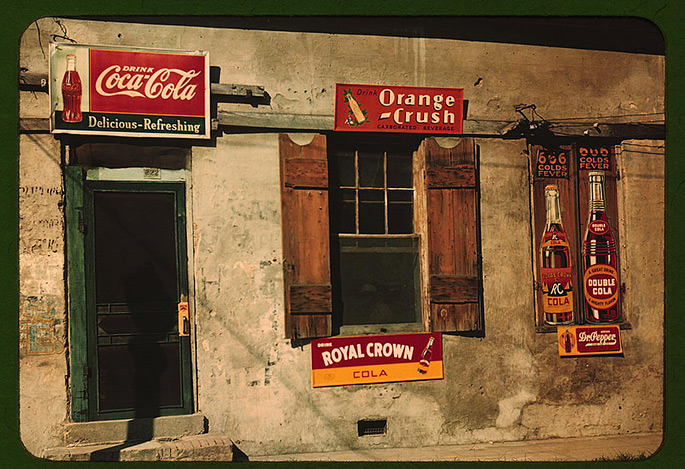
\includegraphics[width=.75\textwidth]{cola-public-domain-photo-p} %{CS0031}
\caption{Coca-Cola Werbung 1940 \cite{CocaCola1940}.}
\label{fig:CocaCola}
\end{figure}


\section{\emph{Let Them Float!}}

Das Platzieren von Abbildungen und Tabellen gehört zu den
schwierigsten Aufgaben im Schriftsatz, weil diese meist viel Platz
benötigen und häufig nicht auf der aktuellen Seite im laufenden
Text untergebracht werden können. Diese Elemente müssen daher an
eine geeignete Stelle auf nachfolgenden Seiten verschoben werden,
was manuell sehr mühsam (jedoch in \emph{Word} beispielsweise unerlässlich) ist.

In \latex funktioniert das weitgehend automatisch, indem
Abbildungen, Tabellen und ähnliche als "Floating Bodies"
behandelt werden. Bei der Positionierung dieser Elemente wird
versucht, einerseits im Textfluss möglichst wenig Leer\-raum
entstehen zu lassen und andererseits die Abbildungen und Tabellen
nicht zu weit von der ursprünglichen Textstelle zu entfernen.

Der Gedanke, dass etwa Abbildungen kaum jemals genau an der
ge\-wünsch\-ten Stelle und möglicherweise nicht einmal auf
derselben Seite Platz finden, ist für viele Anfänger*innen aber offenbar sehr
ungewohnt oder sogar beängstigend. Dennoch sollte zunächst einmal
getrost \latex\ diese Arbeit überlassen und \emph{nicht} manuell
eingegriffen werden. Erst am Ende, wenn das gesamte Dokument "steht" und
die automatische Platzierung wirklich nicht zufriedenstellend erscheint, sollte (durch gezielte Platzierungsanweisungen
\cite[S.~49]{Oetiker2018}) \textbf{in Einzelfällen} eingegriffen werden.



\section{Captions}

Bei Abbildungen steht der Titel üblicherweise \emph{unten}, bei
Tabellen hingegen -- je nach Konvention -- \emph{oben} (wie in diesem Dokument) 
oder ebenfalls \emph{unten}. In \latex\ erfolgt
auch die Nummerierung der Abbildungen automatisch, ebenso der
Eintrag in das (optionale)
Abbildungsverzeichnis%
\footnote{Ein eigenes Verzeichnis der Abbildungen am Anfang des Dokuments
ist zwar leicht erstellt, in einer Abschlussarbeit aber (und eigentlich
überall sonst auch) überflüssig. Man sollte es daher weglassen.}
am Beginn des Dokuments.

Die Markierung der Captions%
\footnote{Ausnahmsweise wird das Wort "Caption" im Folgenden
ohne deutsche Übersetzung verwendet.} erfolgt in \latex mithilfe
der \verb!\label{}! Anweisung, die unmittelbar auf die
\verb!\caption{}! Anweisung folgen muss:
%
\begin{LaTeXCode}[numbers=none]
\begin{figure}
\centering
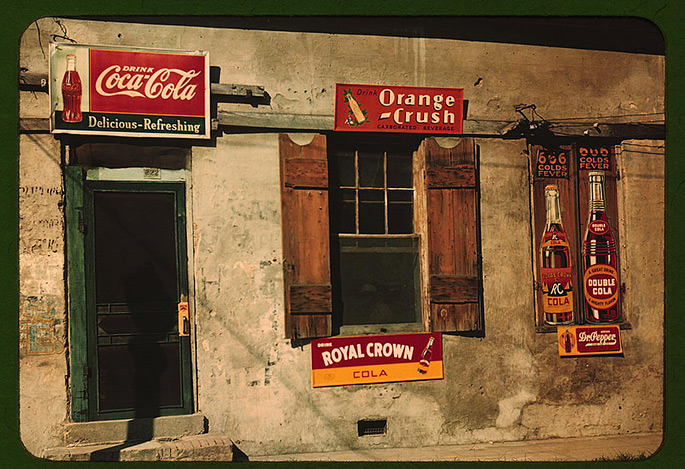
\includegraphics[width=.95\textwidth]{cola-public-domain-photo-p}
\caption{Coca-Cola Werbung 1940 \cite{CocaCola1940}.}
\label{fig:CocaCola}
\end{figure}
\end{LaTeXCode}
%
Der Name des Labels (\texttt{fig:CocaCola}) kann beliebig gewählt werden. 
Die Kennzeichnung \texttt{fig:} ist (wie in Abschn.\ \ref{sec:querverweise} 
erwähnt) nur eine nützliche Hilfe, um beim Schreiben verschiedene Arten 
von Labels besser unterscheiden zu können.

Die Länge der Captions kann dabei sehr unterschiedlich sein. Je
nach Anwendung und Stil ergibt sich manchmal eine sehr kurze
Caption (Abb.~\ref{fig:CocaCola}) oder eine längere
(Abb.~\ref{fig:ibm360}).
Man beachte, wie bei kurzen Captions ein
zentrierter Satz und bei langen Captions ein Blocksatz verwendet
wird (\latex macht das automatisch).
Captions sollten \emph{immer} mit einem Punkt abgeschlossen sein.%
\footnote{Kurioserweise verlangen manche Anleitungen
genau das Gegenteil, angeblich, weil beim klassischen Bleisatz 
die abschließenden Punkte im Druck häufig "weggebrochen" sind. 
Das kann man glauben oder nicht, im Digitaldruck 
spielt es jedenfalls keine Rolle.}

\begin{figure}
\centering
\fbox{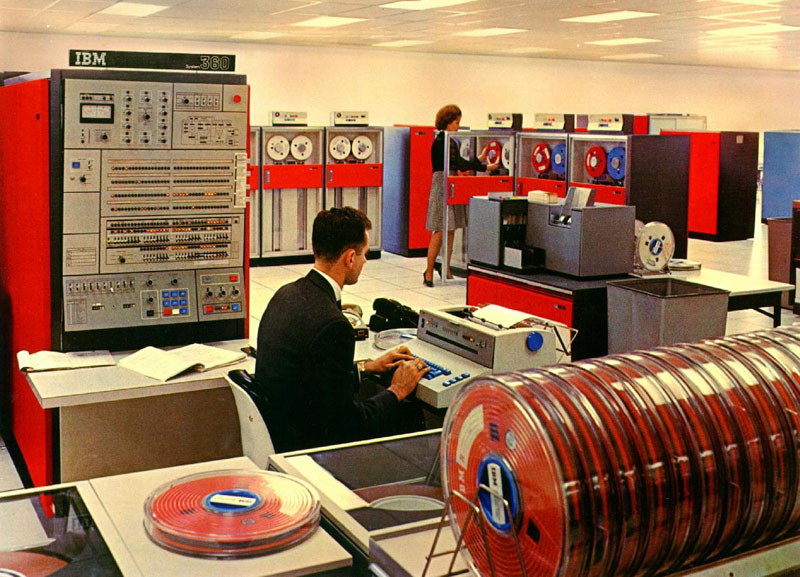
\includegraphics[width=.75\textwidth]{ibm-360-color}}  %{CS1065}}
%\FramePic{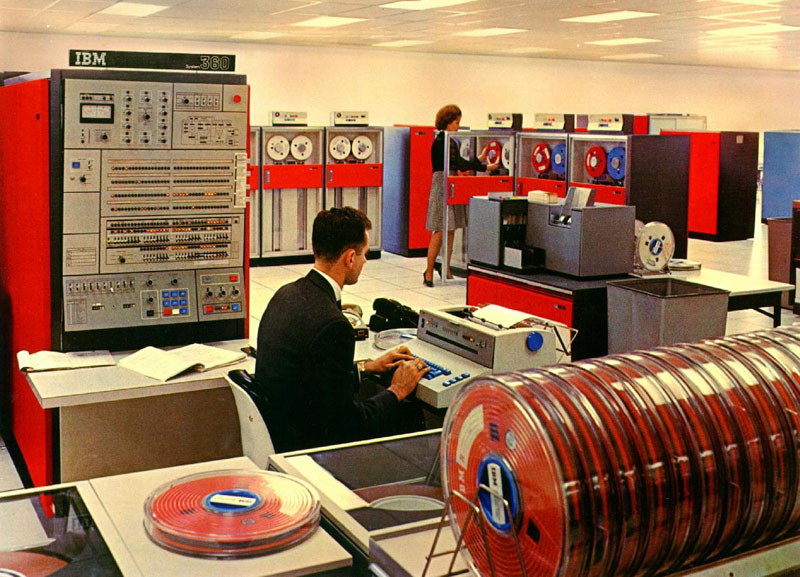
\includegraphics[width=.85\textwidth]{ibm-360-color}} 
\caption{Beispiel für einen langen Caption-Text. \textsc{Univac}
brachte 1961 mit dem Modell 751 den ersten Hochleistungsrechner
mit Halbleiterspeicher auf den Markt. Von diesem Computer wurden
in den U.S.A.\ bereits im ersten Produktionsjahr über fünfzig
Exemplare verkauft, vorwiegend an militärische Dienststellen,
Versicherungen und Großbanken. Die Ablöse erfolgte zwei Jahre
später durch das zusammen mit \textsc{Sperry} entwickelte Modell 820.
Das klingt vielleicht plausibel, ist aber völliger Unsinn, und das
Bild zeigt in Wirklichkeit eine System/360 Anlage von IBM. 
Bildquelle~\cite{IBM360}.} 
\label{fig:ibm360}
\end{figure}





\section{Abbildungen}

Für die Einbindung von Grafiken in \latex wird die Verwendung des Stan\-dard-Pakets
\texttt{graphicx} \cite{Carlisle2020} empfohlen 
(wird durch das \texttt{hagenberg-thesis}-Paket bereits eingebunden). 
Mit dem aktuell verwendeten Workflow (\texttt{pdflatex})
können Bild- bzw.\ Grafikformate ausschließlich 
in folgenden Formaten eingebunden werden:
%
\begin{itemize}
	\item \textbf{PNG}: für Grau-, S/W- und Farb-Rasterbilder (bevorzugt),
	\item \textbf{JPEG}: für Fotos (wenn nicht anders vorhanden),
	\item \textbf{PDF}: für Vektorgrafiken (Illustrationen, Strichzeichnungen \etc).
\end{itemize}
%
Bei Rasterbildern sollte wenn möglich PNG verwendet werden, weil die darin 
enthaltenen Bilder verlustfrei komprimiert sind und daher keine sichtbaren Kompressionsartefakte
aufweisen. Im Gegensatz dazu sollte JPEG nur dann verwendet werden, wenn das Originalmaterial
(Foto) bereits in dieser Form vorliegt.


\subsection{Wo liegen die Grafikdateien?} 

Die Bilder werden üblicherweise in einem Unterverzeichnis (oder in mehreren Unterverzeichnissen) abgelegt,
im Fall dieses Dokuments in \nolinkurl{images/}.
Dazu dient die folgende Anweisung
am Beginn des Hauptdokuments \nolinkurl{main.tex} (\sa\ Anhang \ref{app:latex}):
%
\begin{quote}
\verb!\graphicspath{{images/}}!
\end{quote}
%
Der (zum Hauptdokument relative) Pfad \texttt{graphicspath} kann innerhalb des
Dokuments jederzeit geändert werden, was durchaus nützlich ist, wenn
\zB\ die Grafiken einzelner Kapitel getrennt in entsprechenden Verzeichnissen
abgelegt werden sollen.
Die Größe der Abbildung im Druck kann durch Vorgabe einer bestimmten
Breite oder Höhe oder eines Skalierungsfaktors gesteuert werden, {\zB}:
%
\begin{quote}
\verb!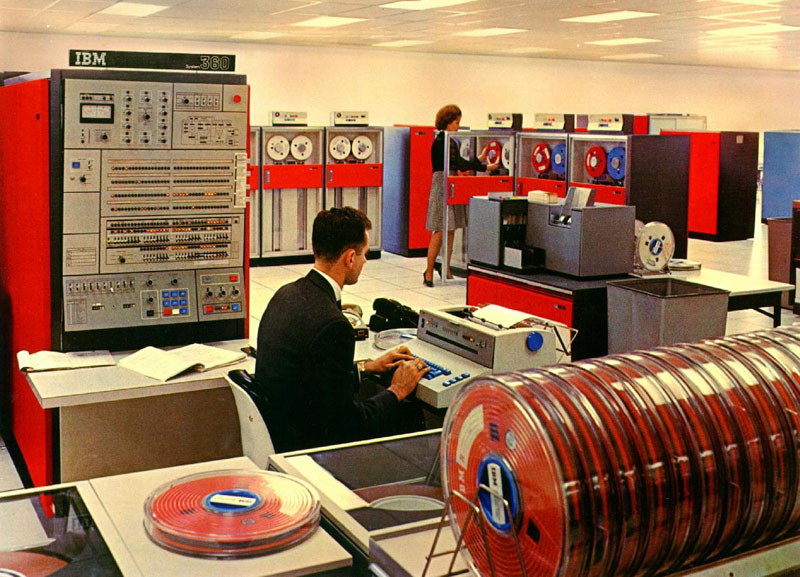
\includegraphics[width=.85\textwidth]{ibm-360-color}! \\
\verb!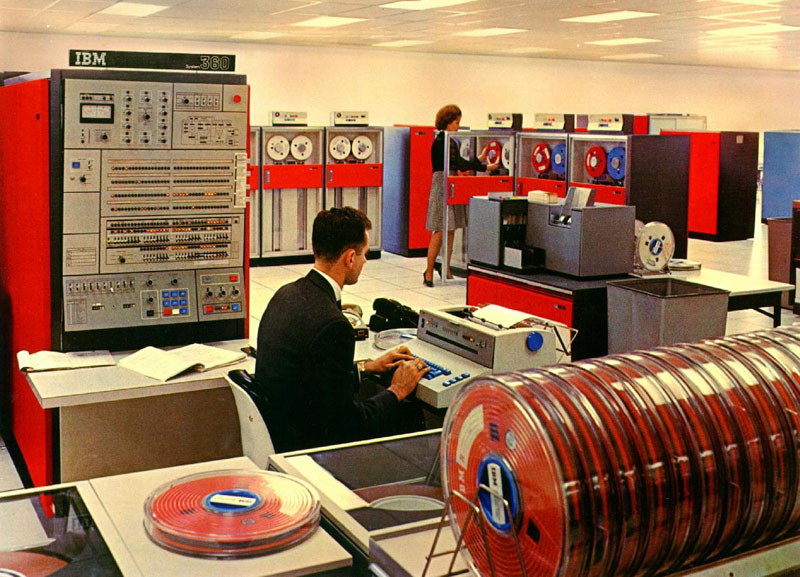
\includegraphics[scale=1.5]{ibm-360-color}!
\end{quote}
%
Man beachte, dass dabei die Dateiendung nicht explizit angegeben werden muss. 
Das ist \va\ dann praktisch, wenn verschiedene Workflows mit jeweils
unterschiedlichen Dateitypen verwendet werden.


\subsection{Grafiken einrahmen} 

%Mit dem Makro \verb!\FramePic{}! (definiert in \texttt{hgb.sty}) kann optional ein dünner 
%Rahmen rund um die Grafik erzeugt werden, \zB:
Mit dem Makro \verb!\fbox{...}! kann optional ein dünner 
Rahmen rund um die Grafik erzeugt werden, \zB:
%
\begin{quote}
%\verb!\FramePic{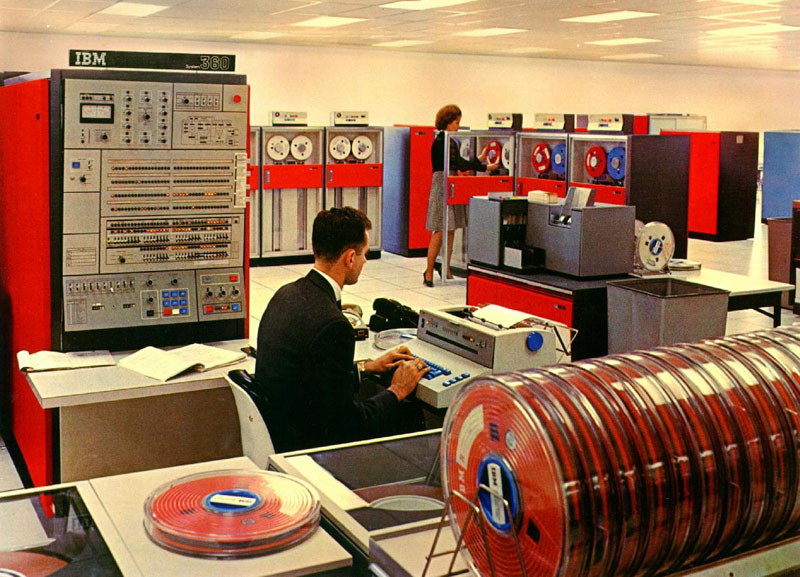
\includegraphics[height=50mm]{ibm-360-color}}!
\verb!\fbox{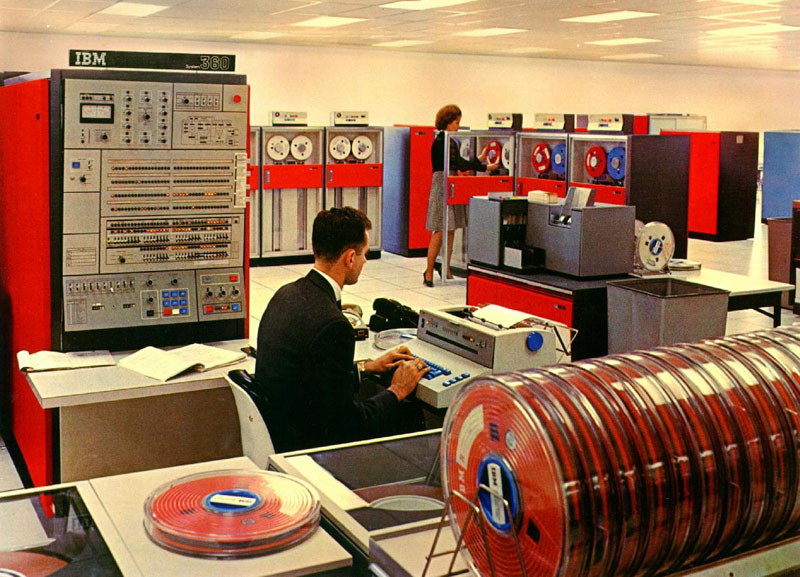
\includegraphics[height=50mm]{ibm-360-color}}!
\end{quote}
%
Das wird üblicherweise nur bei Rasterbildern nötig sein, insbesondere wenn sie zum Rand hin sehr hell sind
und ohne Rahmen nicht vom Hintergrund abgrenzbar wären.

\subsection{Rasterbilder (Pixelgrafiken)}

Generell sollten Bilder bereits vorher so aufbereitet werden,
dass sie später beim Druck möglichst wenig an Qualität verlieren.
Es empfiehlt sich daher, die Bildgröße (Auflösung) bereits im Vorhinein
(\zB mit \emph{Photoshop})
richtig einzustellen.
Brauchbare Auflösungen bezogen auf die endgültige Bildgröße sind:
%
\begin{itemize}
  \item \textbf{Farb- und Grauwertbilder:} 150--300 dpi,
  \item \textbf{Binärbilder (Schwarz/Weiß):} 300--600 dpi.
\end{itemize}
%
Eine wesentlich höhere Auflösung macht aufgrund der beim Laserdruck notwendigen
Rasterung keinen Sinn, auch bei 1200 dpi-Druckern.
Speziell \emph{Screen\-shots} sollten nicht zu klein dargestellt werden,
da sie sonst schlecht lesbar sind (max.\ 200 dpi, besser 150 dpi).
Dabei ist zu bedenken, dass die Arbeit auch als Kopie in allen
Details noch gut lesbar sein sollte.

\subsubsection{JPEG-Problematik}

In der Regel sollten Bilder, die für den Einsatz in
Druckdokumenten gedacht sind, nicht mit verlustbehafteten
Kompressionsverfahren abgespeichert werden. Insbesondere sollte die Verwendung
von JPEG möglichst vermieden werden, auch wenn viele Dateien dadurch
wesentlich kleiner werden. 
Eine Ausnahme ist, wenn die Originaldaten nur in JPEG vorliegen und für die 
Einbindung nicht bearbeitet oder verkleinert wurden. Ansonsten sollte immer
PNG verwendet werden.

Besonders gerne werden farbige \textbf{Screenshots} der JPEG-Kompression%
\footnote{Das JPEG-Verfahren ist für natürliche Fotos konzipiert und sollte auch
nur dafür verwendet werden.}
unter\-zogen, obwohl deren verheerende Folgen für jede*n Laiin*Laien sichtbar sein sollten
(Abb.~\ref{fig:jpeg-pfusch}).

\begin{figure}
\centering\small
\begin{tabular}{@{}cc@{}}
\fbox{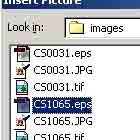
\includegraphics[width=0.475\textwidth]{screenshot-dirty}} &		% JPEG file
\fbox{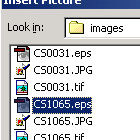
\includegraphics[width=0.475\textwidth]{screenshot-clean}} \\	% PNG file
(a) & (b) 
\end{tabular}
\caption{Typischer JPEG-Pfusch. Screenshots und ähnliche im Original
verfügbare Rasterbilder sollten für Druckdokumente \emph{keinesfalls} mit
JPEG komprimiert werden. Das Ergebnis~(a) sieht gegenüber dem
unkomprimierten Original~(b) nicht nur schmutzig aus, sondern wird
im Druck auch schnell unleserlich.} 
\label{fig:jpeg-pfusch}
\end{figure}



\subsection{Vektorgrafiken}

Für schematische Abbildungen (\zB Flussdiagramme, Entity-Relationship-Diagramme
oder sonstige strukturelle Darstellungen) sollten unbedingt
Vektorgrafiken (PDF) verwendet werden. % (\zB Abb.~\ref{fig:latex-pdf-workflow}).
Gerasterte Grafiken, wie sie üblicherweise als GIF- oder PNG-Dateien
auf Webseiten vorliegen, haben in einem Druckdokument nichts zu suchen, notfalls
müssen sie mit einem entsprechenden Werkzeug \emph{neu} gezeichnet werden (natürlich
unter Angabe der ursprünglichen Quelle).

In diesem Fall kommt als Datenformat nur PDF %(oder EPS im DVI-PS-Workflow) 
in Frage,
dieses bietet sich aber auch in anderen Umgebungen als universelles
Vektor-Format an.
Zur Erstellung von PDF-Vektorgrafiken wird ein geeignetes
Grafikprogramm, \zB\ %\emph{Freehand} von \emph{Macromedia} oder
\emph{Illustrator} von \emph{Adobe} benötigt.
Manche gängigen Grafikprogramme 
unterstützen allerdings keinen direkten Export von PDF-Dateien
oder erzeugen unsaubere Dateien. Vor der Entscheidung
für eine bestimmte Zeichensoftware sollte das im Zweifelsfall
ausprobiert werden.
PDF kann im Notfall über einen entsprechenden Druckertreiber erzeugt werden.


\subsubsection{Vektorgrafiken mit \emph{Inkscape}}
\label{sec:InkscapeGraphics}

Mit \emph{Inkscape}\footnote{\url{https://inkscape.org/}} können Vektorgrafiken auf
sehr einfache Weise erstellt werden.
Das Basisformat von Inkscape ist SVG,
nach dem Export als PDF können solche Grafiken aber wie üblich mit
\verb!\includegraphics[..]{..}! in \latex\ eingefügt werden.

Eine interessante Möglichkeit dabei ist, Texte innerhalb der Grafik
durch \latex\ automatisch ersetzen zu lassen.
Dadurch werden in der fertigen Grafik dieselben Schriften wie im Fließtext
verwendet und \va\ mathematische Elemente entsprechend ersetzt.
Abbildung \ref{fig:InkscapeExample} zeigt ein Beispiel dazu:
%
\begin{itemize}
\item
Die ursprüngliche Inkscape-Grafik \nolinkurl{images/inkscape-template.svg}  enthält
Texte, die nachträglich von \latex\ ersetzt werden sollen 
(siehe Abb.~\ref{fig:InkscapeExample}\,(a)).
\item
Mit Hilfe von \textsf{Save a Copy...} (als PDF) in Inkscape und den Einstellungen wie in 
Abb.~\ref{fig:InkscapeExample}\,(c), werden folgende zwei Files erzeugt:
\begin{itemize}
\item[] \nolinkurl{inkscape-template.pdf}: eine PDF-Datei der Grafik ohne Texte, 
\item[] \nolinkurl{inkscape-template.pdf_tex}: eine \latex-Datei mit allen relevanten Informationen.
\end{itemize}
\end{itemize}
%
Die Einbindung der Grafik in das Dokument erfolgt schließlich durch
\begin{itemize}
\item[] \verb!\input{images/inkscape-template.pdf_tex}!,
\end{itemize}
mit dem in Abb.~\ref{fig:InkscapeExample}\,(b) gezeigten Ergebnis.



\begin{figure}
\centering\small
\begin{tabular}{cc}
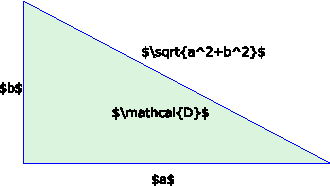
\includegraphics[scale=1.0]{inkscape-template-orig} &
\input{images/inkscape-template.pdf_tex}
\\
(a) & (b)
\\[6pt]
\multicolumn{2}{c}{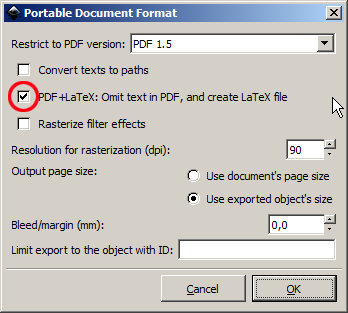
\includegraphics[width=0.4\textwidth]{inkscape-pdf-save-screenhot}%
~~\raisebox{25mm}{(c)}}
\end{tabular}
\caption{Beispiel für eine mit \emph{Inkscape} erzeugte Vektorgrafik
(\nolinkurl{inkscape-template.svg}).
Originalgrafik im \textit{Inkscape}-Editor (a);
beim Einfügen werden die Texte automatisch durch LaTeX ersetzt (b).
Beim Speichern in Inkscape (als PDF) ist auf die Einstellung "PDF+LaTeX" zu achten (c).}
\label{fig:InkscapeExample}
\end{figure}


\subsubsection{Einbettung von Schriften}

Die Wiedergabe von Textelementen ist abhängig von der auf dem
Computer (oder Drucker) installierten Schriften und der Form der
Schrifteinbettung im Quelldokument. Die korrekte Darstellung am
Bildschirm eines Computers bedeutet nicht, dass dasselbe Dokument
auf einem anderen Computer oder Drucker genau so dargestellt wird.
Dieser Umstand ist besonders wichtig, wenn Druckdokumente online
zur Verfügung gestellt werden. Kontrollieren Sie daher genau, ob
die innerhalb Ihrer Grafiken verwendeten Schriften auch exakt wie
beabsichtigt im Ausdruck aufscheinen.


\subsubsection{Strichstärken -- \emph{Hairlines} vermeiden!}

In Grafik-Programmen wie \emph{Inkscape} und \emph{Illustrator},
die sich im Wesentlichen an der \emph{PostScript}-Funktionalität
orientieren, ist es möglich, Linien bzgl.\ ihrer Stärke als
"Hairline" zu definieren. Im zugehörigen \emph{PostScript}-Code
wird dies als \texttt{linewidth} mit dem Wert \texttt{0} ausgedrückt und
sollte am Ausgabegerät "möglichst dünne" Linien ergeben. 
Das Ergebnis ist ausschließlich vom jeweiligen Drucker
abhängig und somit kaum vorhersagbar.
\textbf{Fazit:} Hairlines vermeiden und stattdessen immer konkrete
Strichstärken ($\geq 0.25\,\mathrm{pt}$) einstellen!





\subsection{\tex-Schriften auch in Grafiken?}
\label{sec:tex-schriften-in-grafiken}

Während bei Abbildungen, die mit externen
Grafik-Programmen erzeugt werden, meist mit ähnlich aussehende
Schriften (wie \emph{Times-Roman} oder \emph{Garamond}) Abhilfe schaffen,
besteht bei Purist*innen oft der verständliche Wunsch, die 
\emph{Computer-Modern} (CM) Schriftfamilie von {\tex}/{\latex} auch
innerhalb von eingebetteten Grafiken einzusetzen.

\subsubsection{\emph{BaKoMa}-Schriften (TrueType)}

Glücklicherweise stehen einige Portierungen von CM als {\em
TrueType}-Schriften zur Verfügung, die auch in herkömmlichen
DTP-Anwendungen unter \emph{Windows} und \emph{Mac~OS} verwendet werden
können. Empfehlenswert ist \zB\ die \emph{BaKoMa Fonts Collection},%
\footnote{\url{http://ctan.org/pkg/bakoma-fonts}}
die neben den CM-Standardschriften auch die mathematischen Schriften
der AMS-Familie ent\-hält und zudem kostenfrei ist. Natürlich
müssen die TrueType Schriften vor der Verwendung zunächst auf dem
eigenen PC installiert werden. 


\subsubsection{\emph{Latin Modern Roman} Fonts (OpenType)}

Eine Alternative dazu sind die "LM-Roman"%
\footnote{\url{http://www.gust.org.pl/projects/e-foundry/latin-modern}}
 Open-Type Schriften, die speziell für die Verwendung im Umfeld von \latex\ entwickelt wurden.
Sie sind auch Teil der MikTeX-Installation.%
\footnote{\zB unter \url{C:/Program Files/MiKTeX 2.9/fonts/opentype/public/lm}}
Diese Schriften enthalten \ua\ Zeichen mit Umlauten und sind daher auch für 
deutsche Texte recht bequem zu verwenden.




\subsection{Für Gourmets: Grafiken mit \latex-Overlays}
\label{sec:GraphicOverlays}

Bisweilen ist es erforderlich, ein bestehendes Bilder oder eine Grafik mit 
\latex-eigenen (Vektor-)Elementen zu überlagern, \zB\ für Markierungen
oder Beschriftungen. Ein typisches Beispiel ist in Abb.~\ref{fig:overpic-example}
gezeigt, wo eine mit \emph{Mathematica} generierte PDF-Grafik
mit mathematischen Elementen annotiert wird.


\begin{figure}
\centering\small
%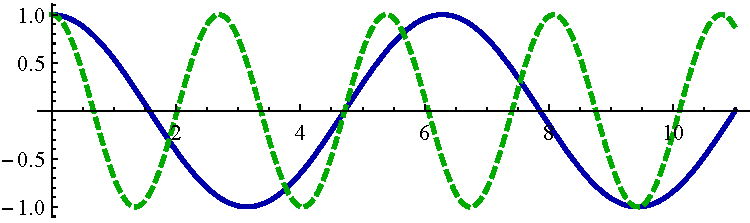
\includegraphics[width=0.85\textwidth]{mathematica-example}
\vspace*{3mm}
\begin{overpic}[width=0.85\textwidth]{mathematica-example}
	\put(101,14){$x$}%
	\put(4,31){$f(x)$}%
	\put(29.5,28){\line(1,1){2}}%
	{\color{green!70!black}\put(29.5,28){\circle*{2.0}}}%
	\put(32,30){$\cos(\frac{7}{3} x)$}%
	\put(59,28){\line(1,1){2}}%
	{\color{blue!70!black}\put(59,28){\circle*{2.0}}}%
	\put(61.5,30){$\cos(x)$}%
\end{overpic}
\caption{Beispiel für die Verwendung des \texttt{overpic}-Pakets zum Einfügen
von \latex-Elementen über eine importierte Grafik.
In diesem Fall wurden die mathematischen Elemente $x$, $f(x)$, $\cos(x)$ und $\smash{\cos(\frac{7}{3} x)}$
sowie zwei diagonale Geraden und gefüllte (färbige) Kreise eingefügt.
Darunter liegt die Vektor\-grafik \texttt{mathematica-example.pdf}.}
\label{fig:overpic-example}
\end{figure}



Dazu wird das \texttt{overpic}-Paket%
\footnote{\url{https://www.ctan.org/pkg/overpic}}
verwendet und zum Importieren der Grafik anstelle von \verb!\includegraphics!
die Umgebung \verb!\begin{overpic}! \ldots \verb!\end{overpic}! verwendet 
(mit ähnlicher Syntax):

\begin{LaTeXCode}[numbers=none]
\begin{overpic}[width=0.85\textwidth]{mathematica-example}
	\put(101,14){$x$}%
	\put(4,31){$f(x)$}%
	\put(29.5,28){\line(1,1){2}}%
	...
\end{overpic}
\end{LaTeXCode}

Die \texttt{overpic}-Umgebung bildet gleichzeitig eine \texttt{picture}-Umgebung, 
in der \latex-Zeichenanweisungen (wie \verb!\put! u.ä.) platziert werden
können, wie in obigem Beispiel gezeigt.\footnote{Die Standard-Zeichenanweisungen
in \latex sind ziemlich restriktiv, weshalb hier zusätzlich das \texttt{pict2e}-Paket
(\url{https://www.ctan.org/pkg/pict2e}) verwendet wird.}
Die $x/y$-Positionen sind in Prozent der Bildbreite angegeben.
Weitere Details finden sich im Quelltext.





\subsection{Abbildungen mit mehreren Elementen}

Werden mehrere Bilder oder Grafiken zu einer Abbildung zusammengefasst, 
wird üblicherweise eine gemeinsame Caption verwendet, wie in Abb.~\ref{fig:Bearings}
dargestellt. Im Text könnte ein Verweis auf einen einzelnen Teil der Abbildung, etwa das 
einreihige Rollenlager in Abb.~\ref{fig:Bearings}\,(c), so aussehen:
%
\begin{LaTeXCode}[numbers=none]
    ... Abb.~\ref{fig:Bearings} (c) ... 
\end{LaTeXCode}


\subsection{Quellenangaben in Captions}
\label{sec:QuellenangabenInCaptions}

Wenn Bilder, Grafiken oder Tabellen aus anderen Quellen verwendet werden, dann 
muss ihre Herkunft in jedem Fall klar ersichtlich gemacht werden, und zwar am 
besten direkt in der Caption.
Wird beispielsweise eine Grafik aus einem Buch oder einer sonstigen 
zitierfähigen Publikation verwendet, dann sollte diese in das Literaturverzeichnis 
aufgenommen und wie üblich mit
\verb!\cite{..}! zitiert werden, wie in Abb.\ \ref{fig:Bearings} demonstriert. 
Weitere Details zu dieser Art von Quellenangaben finden sich in 
Kap.\ \ref{cha:Literatur} (insbes.\ Abschnitt \ref{sec:KategorieOnline}).

\begin{figure}
\centering\small
\begin{tabular}{@{}c@{\hspace{12mm}}c@{}} % mittlerer Abstand = 12mm
  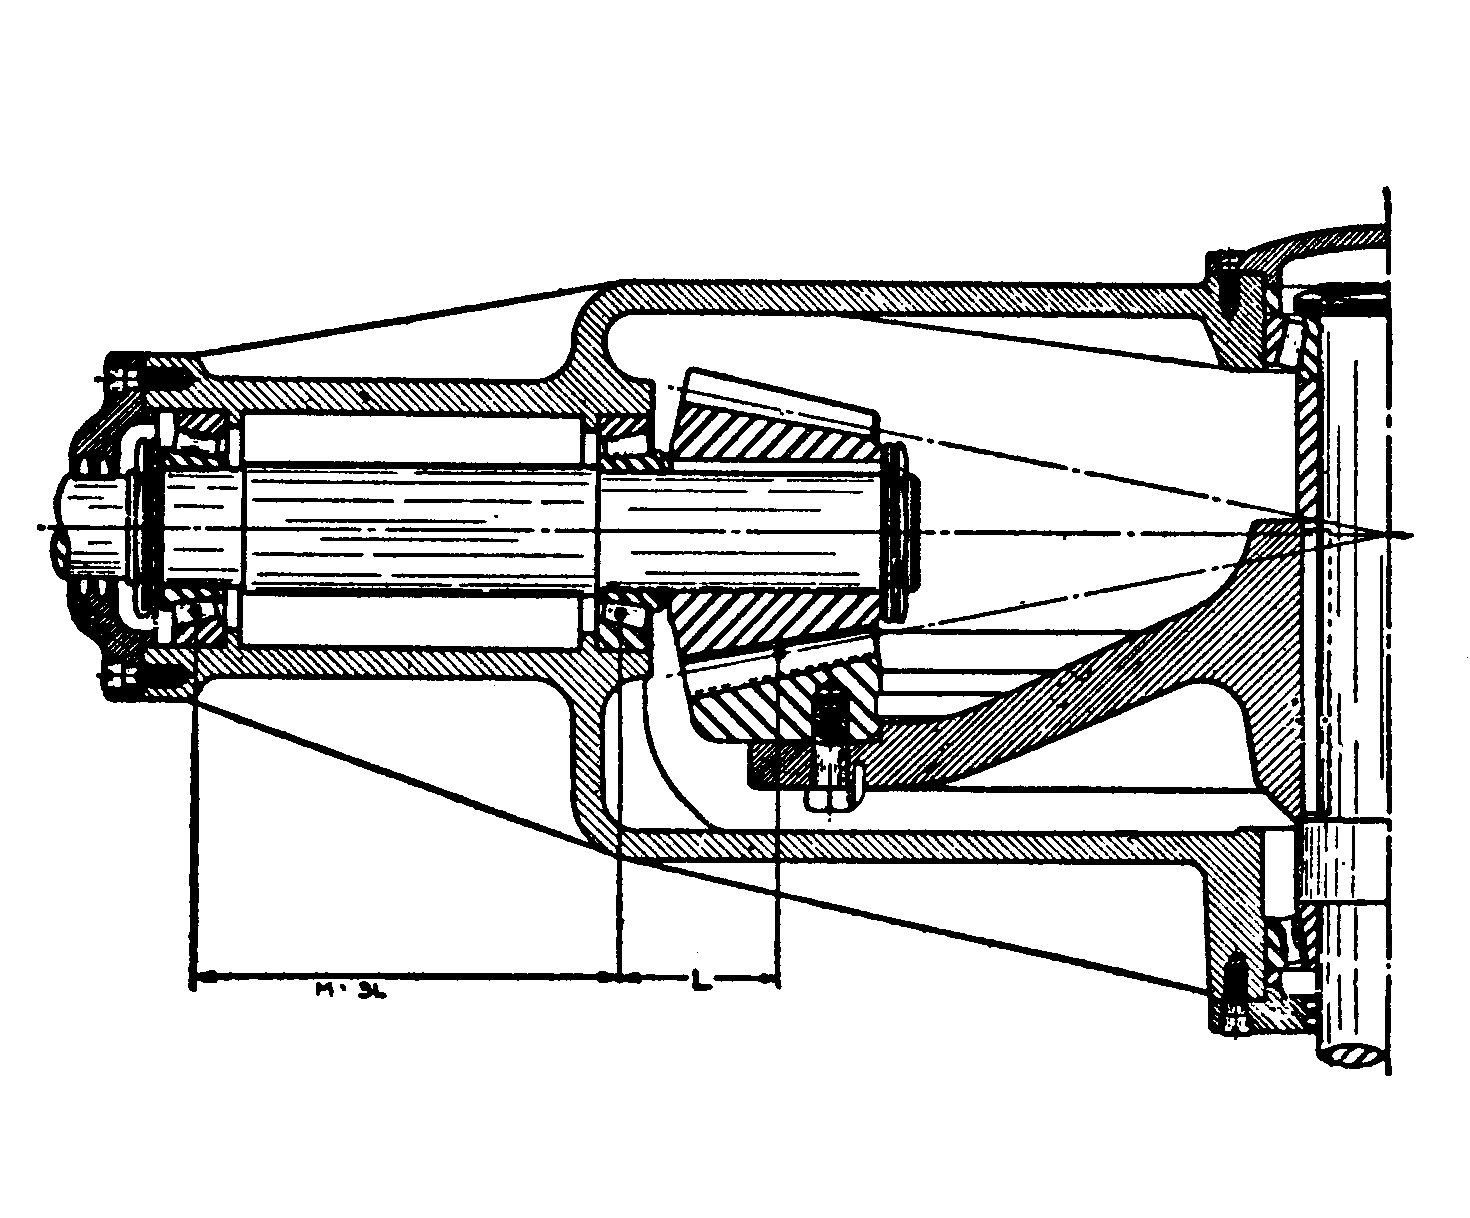
\includegraphics[width=.45\textwidth]{overhang-mounting} &
  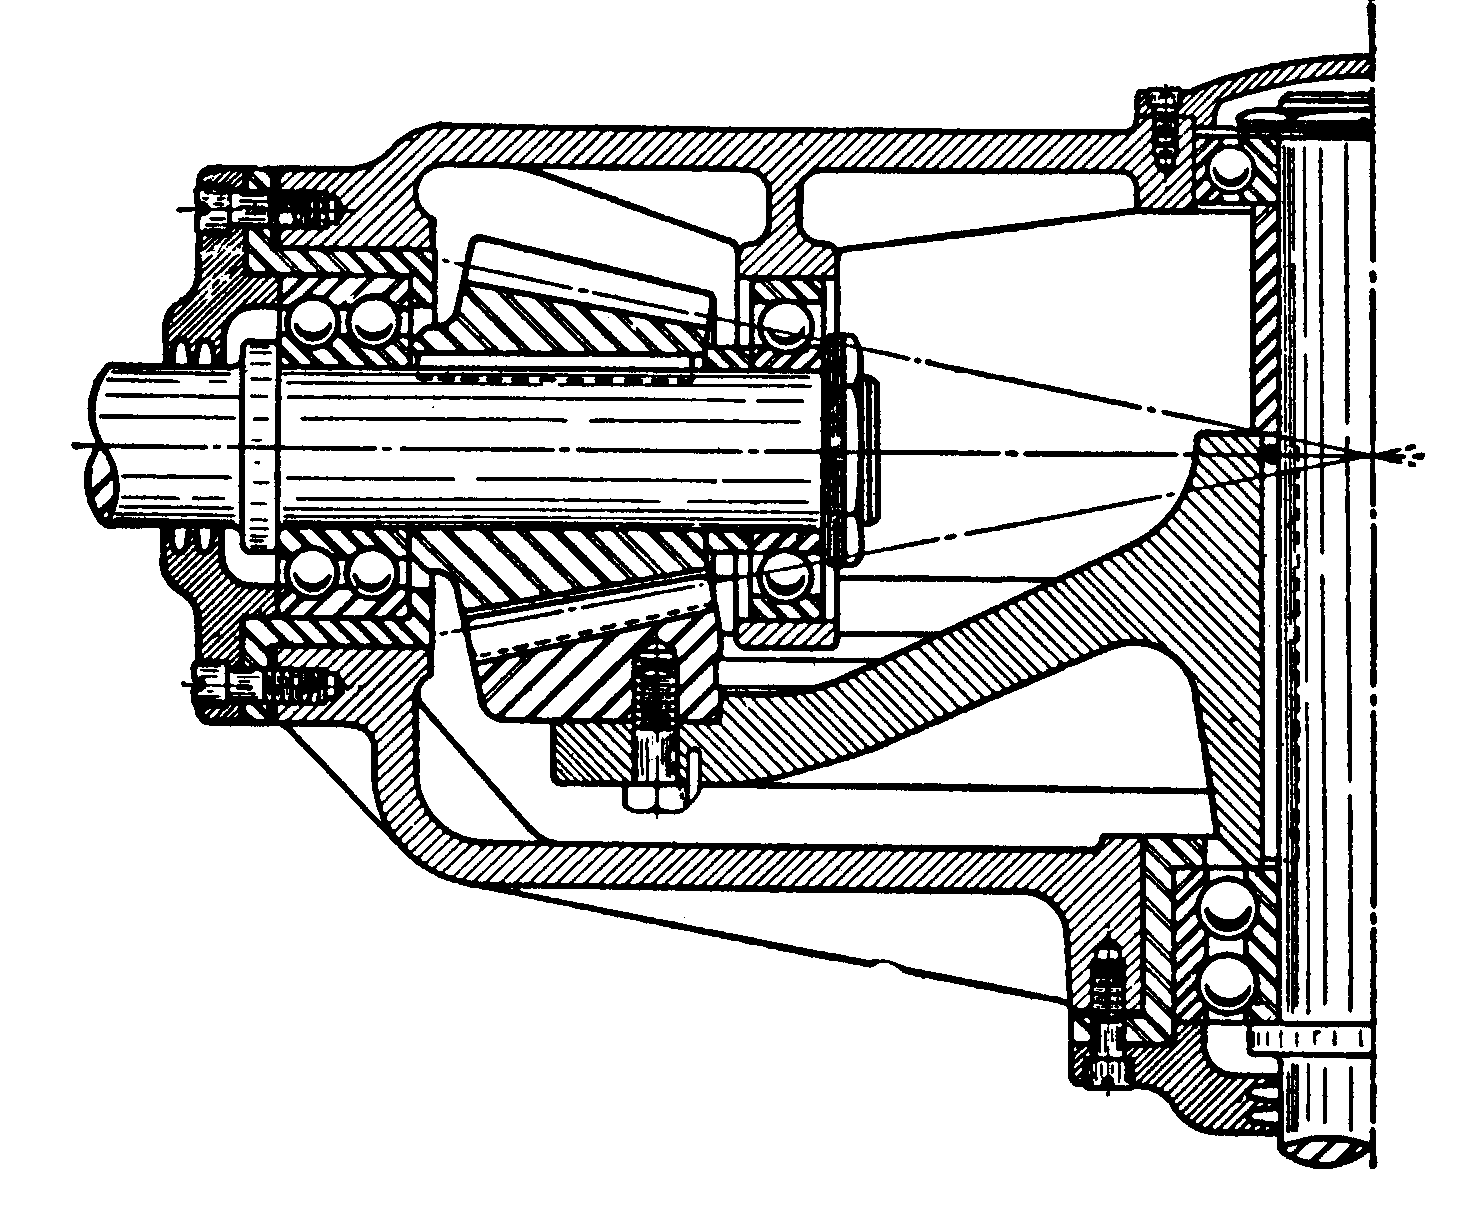
\includegraphics[width=.45\textwidth]{straddle-mounting} 
\\
  (a) & (b)
\\[4pt]	%vertical extra spacing (4 points)
  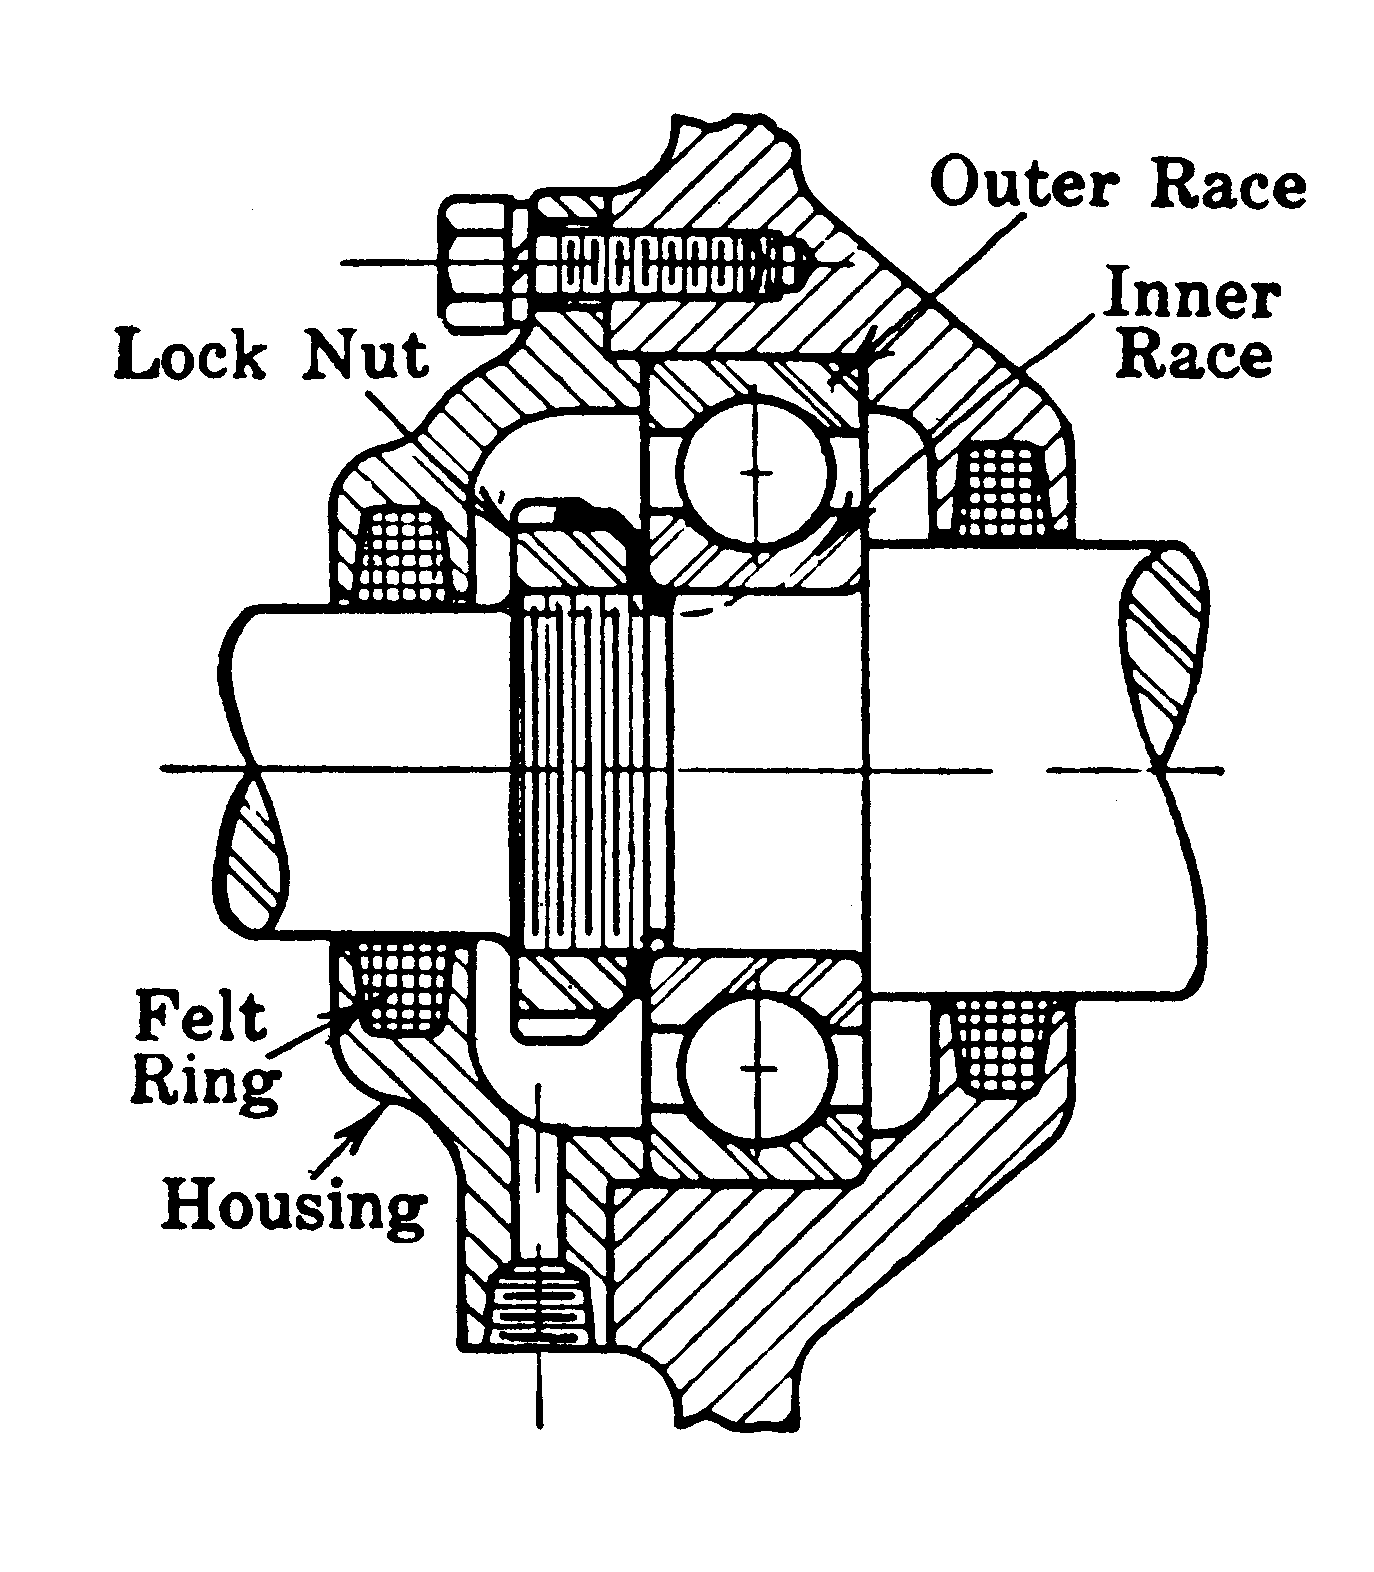
\includegraphics[width=.45\textwidth]{ball-bearing-1} &
  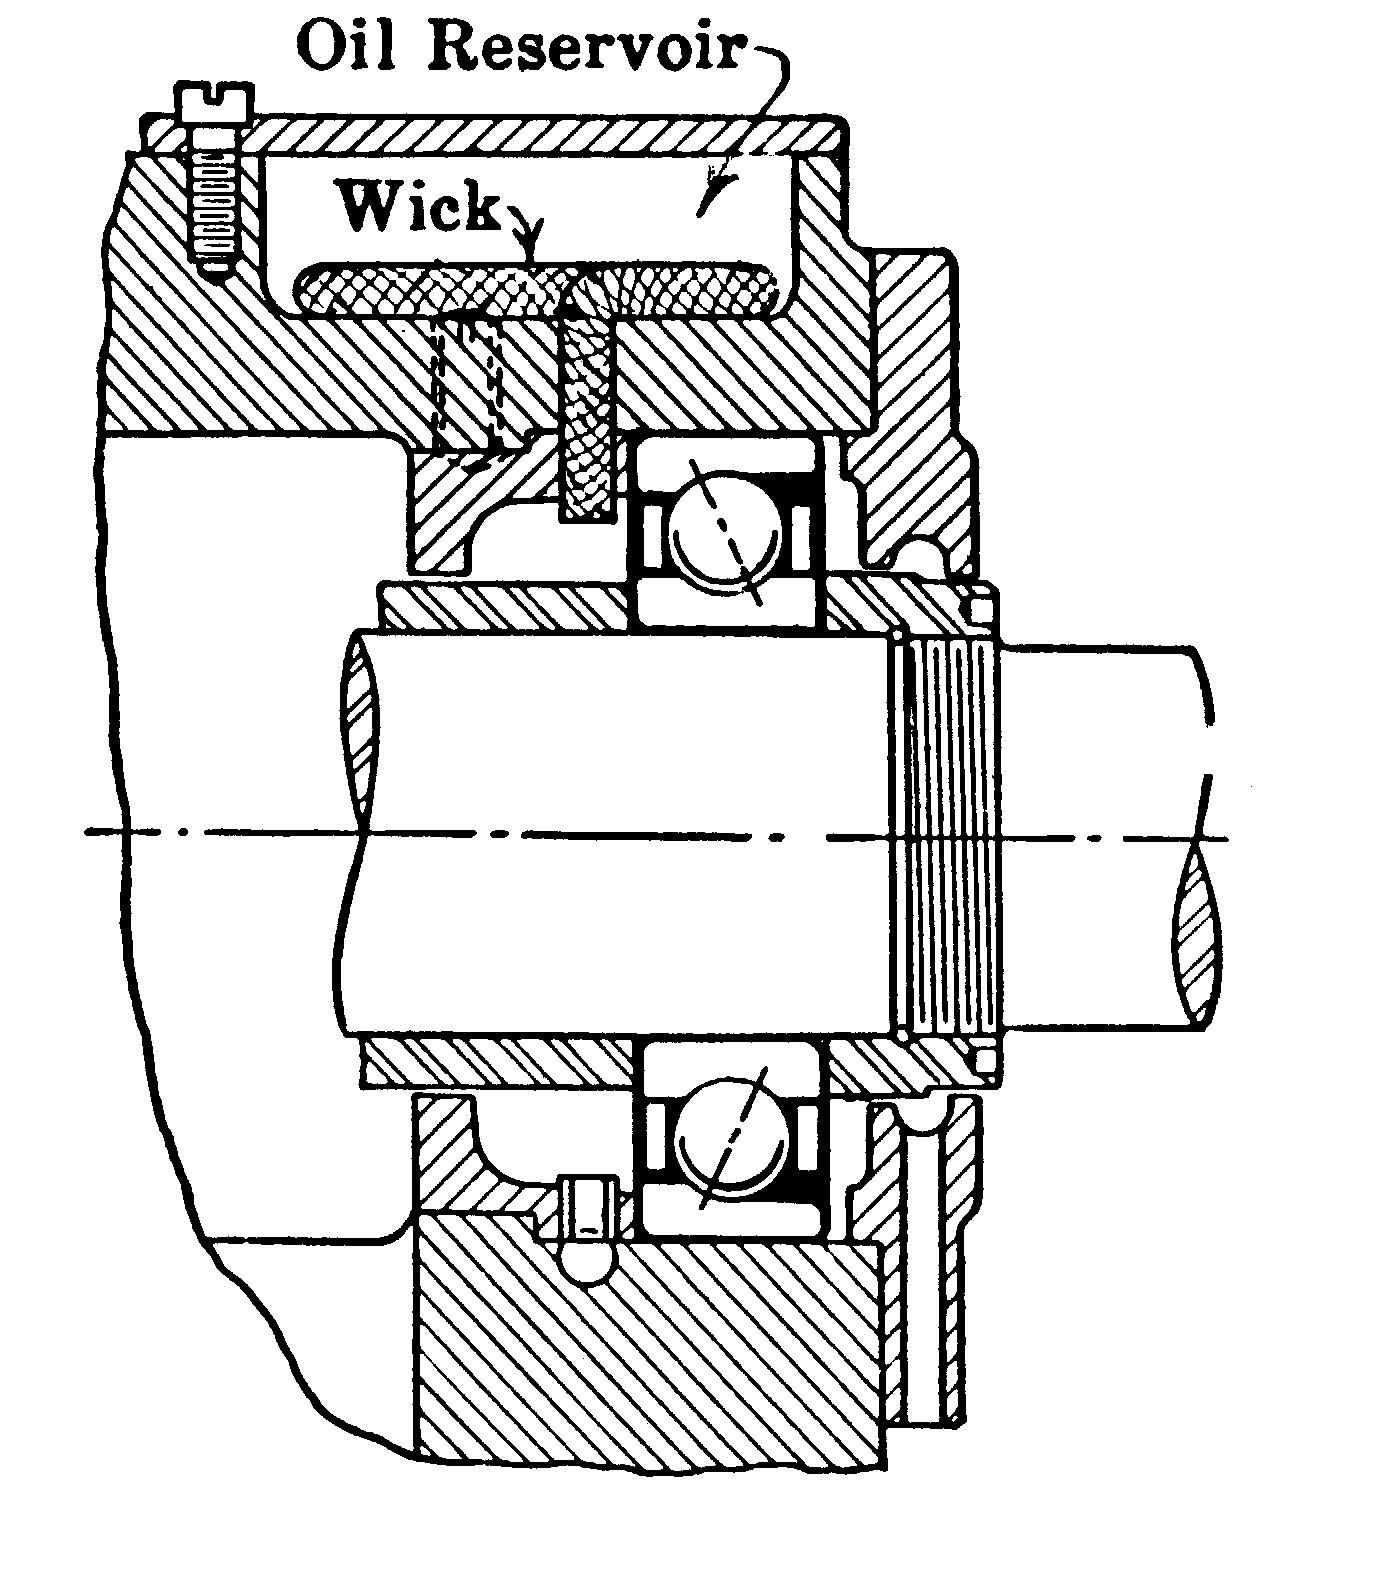
\includegraphics[width=.45\textwidth]{ball-bearing-2} 
\\
  (c) & (d)
\end{tabular}
%
\caption{Diverse Maschinenelemente als Beispiel für eine
Abbildung mit mehreren Elementen.
\emph{Overhang Mounting}~(a), \emph{Straddle Mounting}~(b),
einreihiges Rollenlager~(c), Schmierung von Rollenlagern~(d).
Diese Abbildung verwendet eine gewöhnliche Tabelle (\texttt{tabular}) mit
2 Spalten und 4 Zeilen (Details finden sich im Quelltext).
Bildquelle~\cite{Faires1934}.}
\label{fig:Bearings}
\end{figure}




\section{Tabellen}

Tabellen werden häufig eingesetzt um numerische Zusammenhänge, Testergebnisse
etc.\ in übersichtlicher Form darzustellen.
Ein einfaches Beispiel ist Tab.~\ref{tab:processors}, der \latex-Quelltext dazu
findet sich in Prog.~\ref{prog:processors-source}.


\begin{table}
\caption{Prozessor-Familien im Überblick.}
\label{tab:processors}
\centering
\setlength{\tabcolsep}{5mm}	% separator between columns
\def\arraystretch{1.25}     % vertical stretch factor (Standard = 1.0)
\begin{tabular}{|r||c|c|c|} \hline
& \emph{PowerPC} & \emph{Pentium} & \emph{Athlon} \\
\hline\hline
Manufacturer & Motorola & Intel & AMD \\
\hline
Speed & high & medium & high \\
\hline
Price & high & high  & medium \\
\hline
\end{tabular}
\end{table}

\begin{program}
% place caption consistently either at the top or bottom:
\caption{\latex\ Quelltext zu Tab.~\ref{tab:processors}.
Die Erzeugung des dargestellten Listings selbst ist in Abschn.\ \ref{sec:programmtexte} beschrieben.}
\label{prog:processors-source}
%
\begin{LaTeXCode}[numbers=none]
\begin{table}
	\caption{Prozessor-Familien im Überblick.}
	\label{tab:processors}
	\centering
	\setlength{\tabcolsep}{5mm}	% separator between columns
	\def\arraystretch{1.25}		% vertical stretch factor
	\begin{tabular}{|r||c|c|c|} 
		\hline
		& \emph{PowerPC} & \emph{Pentium} & \emph{Athlon} \\
		\hline
		\hline
		Manufacturer & Motorola & Intel & AMD \\
		\hline
		Speed & high & medium & high \\
		\hline
		Price & high & high & medium \\
		\hline
	\end{tabular}
\end{table}
\end{LaTeXCode}
%
\end{program}

Manchmal ist es notwendig, in Tabellen relativ viel Text in engen Spalten
unter zu bringen, wie in Tab.~\ref{tab:synthesis-techniques}. In diesem Fall
ist es sinnvoll, auf den Blocksatz zu verzichten und gleichzeitig die
strengen Abteilungsregeln zu lockern. Details dazu finden sich im zugehörigen
\latex-Quelltext.


%--------------------------------------------------------------------------------
% Table with narrow columns
%--------------------------------------------------------------------------------
\begin{table}
\caption{Beispiel für eine Tabelle mit mehrzeiligem Text in engen Spalten.
Hier werden die Zeilen für den Blocksatz zu kurz, daher wird linksbündig
gesetzt (im "Flattersatz").}
\label{tab:synthesis-techniques}
\centering
\def\rr{\rightskip=0pt plus1em \spaceskip=.3333em \xspaceskip=.5em\relax}
\setlength{\tabcolsep}{1ex}
\def\arraystretch{1.20}
\setlength{\tabcolsep}{1ex}
\small
\begin{english}
\begin{tabular}{|p{0.2\textwidth}|c|p{0.3\textwidth}|p{0.2\textwidth}|}
\hline
   \multicolumn{1}{|c}{\emph{Method}} &
   \multicolumn{1}{|c}{\emph{Implem.}} &
   \multicolumn{1}{|c}{\emph{Features}} &
   \multicolumn{1}{|c|}{\emph{Status}} \\
\hline\hline
   {\rr polygon shading} &
   SW/HW &
   {\rr flat-shaded polygons} &
   \\
\hline
  {\rr flat shading with z-buffer} &
  SW/HW &
  {\rr depth values} &
  \\
\hline
  {\rr goraud shading with z-buffer} &
  SW/HW &
  {\rr smooth shading, simple fog, point light sources} &
  {\rr SGI entry models} \\
\hline
  {\rr phong shading with z-buffer} &
  SW/HW &
  {\rr highlights} &
  \\
\hline
  {\rr texture mapping with z-buffer} &
  SW/HW &
  {\rr surface textures, simple shadows} &
  {\rr SGI high end, flight simulators} \\
\hline
%  {\rr reflection mapping with z-buffer} &
%  SW/HW &
%  {\rr reflections} &
%  {\rr SGI next generation} \\
%\hline
%  {\rr raytracing} &
%  SW &
%  {\rr refraction, real camera model, area light sources with penumbra, realistic material models} &
%  {\rr common ray\-tracers} \\
%\hline
%  {\rr raytracing + global illumination simulation} &
%  SW &
%  {\rr indirect illumination} &
%  \textit{Radiance} \\
%\hline
%  {\rr raytracing + global illumination simulation + dissipating media} &
%  none &
%  {\rr realistic clouds, scattering, ...} &
%  {\rr research} \\
%\hline
\end{tabular}
\end{english}
\end{table}

%--------------------------------------------------------------------------------



\section{Programmtexte}
\label{sec:programmtexte}

Die Einbindung von Programmtexten (source code) ist eine häufige Notwendigkeit,
\va natürlich bei Arbeiten im Bereich der Informatik.


\subsection{Formatierung von Programmcode}
\label{sec:FormatierungVonProgrammcode}

Es existieren für \latex\ spezielle Pakete zur Darstellung von Programmen, die \ua\ auch die automatische
Nummerierung der Zeilen vornehmen, insbesondere die Pakete \texttt{listings}%
\footnote{\url{https://ctan.org/pkg/listings}}
und \texttt{listingsutf8}.%
\footnote{\url{https://ctan.org/pkg/listingsutf8}}
Damit sind auch die in Tabelle~\ref{tab:CodeUmgebungen} aufgelisteten Code-Umgebungen realisiert.
%
\begin{table}
\caption{In \nolinkurl{hgb.sty} vordefinierte Code-Umgebungen.}
\label{tab:CodeUmgebungen}
\centering
\begin{tabular}{llll}
	\hline
	C (ANSI): & \verb!\begin{CCode}! & \verb!...! \verb!\end{CCode}! \\
	C++ (ISO): & \verb!\begin{CppCode}! & \verb!...! \verb!\end{CppCode}! \\
	C\#: & \verb!\begin{CsCode}! & \verb!...! \verb!\end{CsCode}! \\
	CSS: & \verb!\begin{CssCode}! & \verb!...! \verb!\end{CssCode}! \\
	HTML: & \verb!\begin{HtmlCode}! & \verb!...! \verb!\end{HtmlCode}! \\
	Java: & \verb!\begin{JavaCode}! & \verb!...! \verb!\end{JavaCode}! \\
	JavaScript: & \verb!\begin{JsCode}! & \verb!...! \verb!\end{JsCode}! \\
	\latex: & \verb!\begin{LaTeXCode}! & \verb!...! \verb!\end{LaTeXCode}! \\
	Objective-C: & \verb!\begin{ObjCCode}! & \verb!...! \verb!\end{ObjCCode}! \\
	PHP: & \verb!\begin{PhpCode}! & \verb!...! \verb!\end{PhpCode}! \\
	Python: & \verb!\begin{PythonCode}! & \verb!...! \verb!\end{PythonCode}! \\
	Swift: & \verb!\begin{SwiftCode}! & \verb!...! \verb!\end{SwiftCode}! \\
	XML: & \verb!\begin{XmlCode}! & \verb!...! \verb!\end{XmlCode}! \\
	Generisch: & \verb!\begin{GenericCode}! & \verb!...! \verb!\end{GenericCode}! \\
	\hline
\end{tabular}
\end{table}
%
Die Verwendung ist äußerst einfach, \zB\ für Quellcode in der Programmiersprache C schreibt man
%
\begin{quote}
\begin{verbatim}
\begin{CCode}
    ... 
\end{CCode}
\end{verbatim}
\end{quote}
%
Der Quellcode innerhalb dieser Umgebungen wird in der jeweiligen Programmiersprache interpretiert, wobei Kommentare erhalten bleiben. Diese Umgebungen können sowohl alleinstehend (im Fließtext) oder innerhalb von Float-Umgebungen (insbes.\ \texttt{program}) verwendet werden. Im ersten Fall wird der Quelltext auch über Seitengrenzen umgebrochen. Mit \verb!/+! ... \verb!+/! ist eine Escape-Möglichkeit nach \latex\ vorgesehen, die \va\ zum Setzen von Labels für Verweise auf einzelne Programmzeilen nützlich ist, \zB\ mit
%
\begin{quote}
\verb!/+\label{ExampleCodeLabel}+/!
\end{quote}
%
Ein Beispiel mit Java ist in Prog.~\ref{prog:CodeExample} gezeigt, wobei der oben angeführte Label in Zeile \ref{ExampleCodeLabel} steht.
Man beachte, dass innerhalb der Kommentare auch mathematischer Text 
(wie etwa in Zeile \ref{MathInCode} von Prog.~\ref{prog:CodeExample}) stehen kann.


\subsubsection{Nummerierung der Code-Zeilen}

Alle in Tabelle~\ref{tab:CodeUmgebungen} angeführten Code-Umgebungen können
mit optionalen Argumenten verwendet werden, die insbesondere zur Steuerung der
Zeilennummerierung hilfreich. 
Im Normalfall (also ohne zusätzliche Angabe) mit
%
\begin{quote}
\verb!\begin{!\texttt{\emph{some}Code}\verb!} ... !
\end{quote}
%
werden alle Code-Zeilen (einschließlich der Leerzeilen) bei 1 beginnend und 
fortlaufend nummeriert.
%
Bei aufeinanderfolgenden Codesegmenten ist es oft hilfreich, die Nummerierung 
aus dem vorherigen Abschnitt kontinuierlich weiter laufen zu lassen,
ermöglicht durch die Angabe des optionalen Arguments 
\texttt{firstnumber={\obnh}last}:
%
\begin{quote}
\verb!\begin{!\texttt{\emph{some}Code}\verb!}[firstnumber=last] ... !
\end{quote}
%
Um die Nummerierung der Codezeilen gänzlich zu unterbinden genügt die Angabe
des optionalen Arguments
\texttt{numbers={\obnh}none}:
%
\begin{quote}
\verb!\begin{!\texttt{\emph{some}Code}\verb!}[numbers=none] ... !
\end{quote}
%
In diesem Fall ist natürlich die Verwendung von Zeilenlabels im Code nicht
sinnvoll.


\subsection{Platzierung von Programmcode}

Da Quelltexte sehr umfangreich werden können, ist diese Aufgabe nicht
immer leicht zu lösen. Abhängig vom Umfang und vom Bezug zum Haupttext
gibt es grundsätzlich drei Möglichkeiten zur Einbindung von Programmtext:
%
\begin{itemize}
\item[a)] im laufenden Text für kurze Programmstücke,
\item[b)] als Float-Element (\texttt{program}) für mittlere Programmtexte bis max.\ eine Seite oder
\item[c)] im Anhang (für lange Programmtexte).
\end{itemize}

\subsubsection{Programmtext im laufenden Text}

Kurze Codesequenzen können ohne weiteres im laufenden Text
eingebettet werden, sofern sie an den gegebenen Stellen von unmittelbarer
Bedeutung sind. Die folgende (rudimentäre) Java-Methode \texttt{extractEmail} sucht
nach einer E-Mail-Adresse in der Zeichenkette
\texttt{line}:
%
\begin{JavaCode}[numbers=none]
static String extractEmail(String line) {
    line = line.trim(); // find the first blank
    int i = line.indexOf(' '); 
    if (i > 0)
        return line.substring(i).trim();
    else
        return null;
}
\end{JavaCode}
\medskip

\noindent
Dieses Codestück wurde mit 
%
\begin{quote}
\begin{verbatim}
\begin{JavaCode}[numbers=none]
static String extractEmail(String line) {
    line = line.trim(); // find the first blank
    ...
}
\end{JavaCode}
\end{verbatim}
\end{quote}
%
erstellt (siehe Abschn.\ \ref{sec:FormatierungVonProgrammcode}). 
In-line Programmstücke sollten maximal einige Zeilen lang sein und 
nach Möglichkeit nicht durch Seitenumbrüche geteilt werden.
%Um auch längere Programmzeilen unterzubringen, empfiehlt es sich, dafür
%eine entsprechend kleine Schriftgröße zu wählen (als Standardgröße ist
%\texttt{footnotesize} eingestellt). 


\subsubsection{Programmtexte als Float-Elemente}
Sind längere Codesequenzen notwendig, die in unmittelbarer Nähe des laufenden Texts
stehen müssen, sollten diese genauso wie andere Abbildungen als Float-Elemente
behandelt werden. Diese Programmtexte sollten den Umfang von einer Seite nicht übersteigen.
Im Notfall können auch bis zu zwei Seiten in aufeinanderfolgende Abbildungen gepackt werden,
jeweils mit eigener Caption. In \texttt{hgb.sty} ist eine neue Float-Umgebung \texttt{program} definiert, die analog zu \texttt{table} verwendet wird:
%
\begin{quote}
\begin{verbatim}
\begin{program}
\caption{Der Titel zu diesem Programmstück.}
\label{prog:xyz}
\begin{JavaCode}
  class IrgendWas {
    ...
  }
\end{JavaCode}
\end{program}
\end{verbatim}
\end{quote}
%
Wenn gewünscht, kann die Caption auch unten angebracht werden 
(jedenfalls aber konsistent und nicht gemischt).
Natürlich darf auch hier nicht mit einer linearen Abfolge im fertigen
Druckbild gerechnet werden, daher sind Wendungen wie
"\ldots\ im folgenden Programmstück \ldots" zu vermeiden und entsprechende Verweise
einzusetzen. Beispiele sind die Programme \ref{prog:processors-source} und \ref{prog:CodeExample}.

\begin{program}
% place caption consistently either at the top or bottom:
\caption{Beispiel für die Auflistung von Programmcode als Float-Element.}
\label{prog:CodeExample}
\begin{JavaCode}
import ij.ImagePlus;
import ij.plugin.filter.PlugInFilter;
import ij.process.ImageProcessor;

public class My_Inverter implements PlugInFilter {
	int agent_velocity;
  String title = ""; // just to test printing of double quotes

	public int setup (String arg, ImagePlus im) {
		return DOES_8G;	// this plugin accepts 8-bit grayscale images /+\label{pr:IjSamplePlugin10}+/
	}

	public void run (ImageProcessor ip) {
		int w = ip.getWidth();	/+\label{ExampleCodeLabel}+/
		int h = ip.getHeight(); 
		
		/* iterate over all image coordinates */
		for (int u = 0; u < w; u++) { 
			for (int v = 0; v < h; v++) {
				int p = ip.getPixel(u, v); 
				ip.putPixel(u, v, 255-p); // invert: /+$I'(u,v) \leftarrow 255 - I(u,v)$\label{MathInCode}+/
			}
		}
	}		
} // end of class My_Inverter
\end{JavaCode}
%
\end{program}


\subsubsection{Programmtext im Anhang}

Für längere Programmtexte, speziell wenn sie vollständige
Implementierungen umfassen und im aktuellen Kontext nicht
unmittelbar relevant sind, muss zur Ablage in einem getrennten
Anhang am Ende des Dokuments gegriffen werden. Für Hinweise auf bestimmte
Details können entweder kurze Ausschnitte in den laufenden Text
gestellt oder mit entsprechenden Seitenverweisen gearbeitet werden. Ein
solches Beispiel ist der \latex-Quellcode in Anhang
\ref{app:latex} (Seite \pageref{app:latex}).%
\footnote{%
Grundsätzlich ist zu überlegen, ob die gedruckte Einbindung der gesamten
Programmtexte einer Implementierung für den*die Leser*in überhaupt sinnvoll ist, oder
ob diese nicht besser elektronisch (auf Datenträger) beigefügt und nur exemplarisch
beschrieben werden.}

\chapter[Mathem.\ Formeln etc.]{Mathematische Formeln, Gleichungen und Algorithmen}
\label{cha:Mathematik}



Das Formatieren von mathematischen Elementen gehört sicher zu den
Stär\-ken von \latex. Man unterscheidet zwischen mathematischen Elementen
im Fließtext und freistehenden Gleichungen, die in der Regel
fortlaufend nummeriert werden. Analog zu Abbildungen und Tabellen sind dadurch
Querverweise zu Gleichungen leicht zu realisieren.
Hier nur einige Beispiele und spezielle Themen, vieles weitere dazu findet sich \zB in
\cite[Kap.\ 7]{Kopka2003} und~\cite{Voss2014}.


\section{Mathematische Elemente im Fließtext}

Mathematische Symbole, Ausdrücke, Gleichungen etc.\ werden im Fließtext durch paarweise 
\verb!$! \ldots \verb!$! markiert. Hier ein simples Beispiel:
%
\begin{itemize}
\item[]
Der Nah-Unendlichkeitspunkt liegt bei
$\bar{a} = f' \cdot (f' / (K \cdot u_{\max}) + 1)$,
sodass bei einem auf $\infty$ eingestellten Objektiv von der Entfernung
$\bar{a}$ an alles scharf ist. Fokussiert man das
Objektiv auf die Entfernung $\bar{a}$ (\dah, $a_0 = \bar{a}$), dann wird
im Bereich $[\frac{\bar{a}}{2}, \infty]$ alles scharf.
\end{itemize}
%
Dabei sollte unbedingt darauf geachtet werden, dass die Höhe der einzelnen Elemente im Text nicht zu groß wird. 

\paragraph{Häufiger Fehler:} 
Im Fließtext wird bei einfachen Variablen oft auf die Verwendung der richtigen, mathematischen
Zeichen vergessen, wie etwa in "X-Achse" anstelle von "$X$-Achse" (\verb!$X$-Achse!).

\paragraph{Zeilenumbrüche:}
Bei längeren mathematischen Elementen im Fließtext sind Probleme mit Zeilenumbrüchen
vorprogrammiert. In der Regel ermöglicht \latex nur am "=" einen Zeilenumbruch,
an anderer Stelle kann man Umbrüche mit \texttt{{\bs}allowbreak} ermöglichen. 
Hier ein kleines Beispiel:
%
\begin{itemize}
\item[a)] Einen einfachen Zeilenvektor definiert man beispielsweise in der Form 
		$\boldsymbol{x} = (x_0, x_1, \ldots, x_{n-1})$.
\item[b)] Einen einfachen Zeilenvektor definiert man beispielsweise in der Form 
	$\boldsymbol{x} = (x_0,\allowbreak x_1,\allowbreak\ldots,\allowbreak x_{n-1})$.
\end{itemize}
Die Zeile in a) sollte über den Seitenrand hinauslaufen, b) hingegen enthält
\texttt{{\bs}allowbreak} an mehreren Stellen und sollte daher sauber umbrechen.


\section{Freigestellte Ausdrücke}

Freigestellte mathematische Ausdrücke können in \latex\ im einfachsten Fall durch paarweise 
\verb!$$! \ldots \verb!$$! erzeugt werden. Das Ergebnis wird zentriert, erhält jedoch keine 
Nummerierung. So ist \zB\ $$y = 4 x^2$$ das Ergebnis von \verb!$$y = 4 x^2$$!.


\subsection{Einfache Gleichungen} 

Meistens wird in solchen Fällen jedoch die \texttt{equation}-Umgebung zur Herstellung nummerierter 
Gleichungen verwendet, auf die im Text jederzeit verwiesen werden kann. Zum Beispiel erzeugt
%
\begin{LaTeXCode}[numbers=none]
\begin{equation}
  f(k) = \frac{1}{N} \sum_{i=0}^{k-1} i^2 . 
  \label{eq:MyFirstEquation}
\end{equation}
\end{LaTeXCode}
%
die Gleichung
%
\begin{equation}
  f(k) = \frac{1}{N} \sum_{i=0}^{k-1} i^2 . 
\label{eq:MyFirstEquation}
\end{equation}
%
Mit \verb!\ref{eq:MyFirstEquation}! erhält man wie üblich die Nummer (\ref{eq:MyFirstEquation}) dieser Gleichung (siehe dazu auch Abschn.\ \ref{sec:VerweiseAufGleichungen}). 
Dieselbe Gleichung \emph{ohne} Nummerierung kann übrigens mit der \texttt{equation*}-Umgebung erzeugt werden.



\begin{center}
\setlength{\fboxrule}{0.2mm}
\setlength{\fboxsep}{2mm}
\fbox{%
\begin{minipage}{0.9\textwidth}
Man beachte, dass \textbf{Gleichungen} inhaltlich ein \textbf{Teil des Texts} sind und daher neben der sprachlichen
\textbf{Überleitung} auch die \textbf{Interpunktion} (wie in Gl.\ \ref{eq:MyFirstEquation} gezeigt) beachtet werden muss. 
Bei Unsicherheiten sollte man sich passende Beispiele in einem guten Mathematik\-buch ansehen.
\end{minipage}}
\end{center}
%
Für Interessierte findet sich mehr zum Thema Mathematik und Prosa in \cite{Mermin1989} und \cite{Higham1998}.

\subsection{Mehrzeilige Gleichungen}

Für mehrzeilige Gleichungen bietet \latex\ die 
\verb!eqnarray!-Umgebung, die allerdings etwas eigenwillige Zwischenräume erzeugt.
Es empfiehlt sich, dafür gleich auf die erweiterten Möglichkeiten des \texttt{amsmath}-Pakets%
\footnote{American Mathematical Society (AMS). \texttt{amsmath} ist Teil der \latex\ Standardinstallation und wird von \texttt{hgb.sty} bereits importiert.}
\cite{Mittelbach2018} zurückzugreifen.
Hier ein Beispiel mit zwei am $=$ Zeichen ausgerichteten Gleichungen,
%
\begin{align}
f_1 (x,y) &= \frac{1}{1-x} + y , \label{eq:f1} \\
f_2 (x,y) &= \frac{1}{1+y} - x , \label{eq:f2}
\end{align}
%
erzeugt mit der \texttt{align}-Umgebung aus dem \texttt{amsmath}-Paket:
%
\begin{LaTeXCode}[numbers=none]
\begin{align}
  f_1 (x,y) &= \frac{1}{1-x} + y , \label{eq:f1} \\
  f_2 (x,y) &= \frac{1}{1+y} - x , \label{eq:f2}
\end{align}
\end{LaTeXCode}


\subsection{Fallunterscheidungen}

Mit der \texttt{cases}-Umgebung aus \texttt{amsmath} sind Fallunterscheidungen, \ua\ innerhalb von Funktionsdefinitionen, sehr einfach zu bewerkstelligen. Beispielsweise wurde die rekursive Definition
%
\begin{equation}
	f(i) =
	\begin{cases}
	  0             & \text{für $i = 0$,}\\
	  f(i-1) + f(i) & \text{für $i > 0$.}
	\end{cases}
\end{equation}
mit folgenden Anweisungen erzeugt:
%
\begin{LaTeXCode}[numbers=none]
\begin{equation}
	f(i) =
	\begin{cases}
	  0             & \text{für $i = 0$,}\\
	  f(i-1) + f(i) & \text{für $i > 0$.}
	\end{cases}
\end{equation}
\end{LaTeXCode}
%
Man beachte dabei die Verwendung des sehr praktischen \verb!\text{..}!-Makros, mit dem im Mathematik-Modus gewöhnlicher Text eingefügt werden kann, sowie wiederum die Interpunktion innerhalb der Gleichung.


\subsection{Gleichungen mit Matrizen}

Auch hier bietet \texttt{amsmath} einige Vorteile gegenüber der Verwendung der \latex\ Standardkonstrukte. Dazu ein einfaches Beispiel für die Verwendung der \texttt{pmatrix}-Umgebung für Vektoren und Matrizen,
%
\begin{equation}
	\begin{pmatrix} x' \\ y' \end{pmatrix}
	= 
	\begin{pmatrix}
	  \cos \phi & -\sin \phi \\
	  \sin \phi & \phantom{-}\cos \phi
	\end{pmatrix} 
	\cdot
	\begin{pmatrix}	x \\ y \end{pmatrix} ,
\end{equation}
%
das mit den folgenden Anweisungen erzeugt wurde:
%
\begin{LaTeXCode}
\begin{equation}
	\begin{pmatrix} 
			x' \\ 
			y' 
	\end{pmatrix}
	= 
	\begin{pmatrix}
		  \cos \phi &           -\sin \phi \\
		  \sin \phi & \phantom{-}\cos \phi /+ \label{lin:phantom} +/
	\end{pmatrix} 
	\cdot
	\begin{pmatrix} 
			x \\ 
			y 
	\end{pmatrix} ,
\end{equation}
\end{LaTeXCode}
%
Ein nützliches Detail darin ist das \tex-Makro \verb!\phantom{..}! (in Zeile \ref{lin:phantom}), das sein Argument unsichtbar einfügt und hier als Platzhalter für das darüberliegende Minuszeichen verwendet wird. Alternativ zu \texttt{pmatrix} kann mit der \texttt{bmatrix}-Umgebung Matrizen
und Vektoren mit eckigen Klammern erzeugt werden.
Zahlreiche weitere mathematische Konstrukte des \texttt{amsmath}-Pakets sind in \cite{Mittelbach2018} beschrieben.

\begin{comment}
% Umsetzung ohne amsmath:
\begin{equation}
\left[ \begin{array}{c}
  x' \\ y'
\end{array} \right] 
= 
\left[ \begin{array}{rr}
	 \cos \phi & \sin \phi \\
	-\sin \phi & \cos \phi
\end{array} \right] 
\cdot
\left[ \begin{array}{c}
	x \\ y
\end{array}
\right] 
.
\end{equation}
\end{comment}



\subsection{Verweise auf Gleichungen}
\label{sec:VerweiseAufGleichungen}

Beim Verweis auf nummerierte Formeln und Gleichungen genügt grundsätzlich die Angabe 
der entsprechenden Nummer in runden Klammern,
\zB\
\begin{center}
%"\ldots\ wie aus (\ref{eq:f1}) abgeleitet werden kann \ldots"
"\ldots\ wie aus (\ref{eq:f1}) abgeleitet werden kann \ldots"
\end{center}
Um Missverständnisse zu vermeiden, sollte aber -- \va\ in Texten mit
nur wenigen mathematischen Elementen -- "Gleichung \ref{eq:f1}", "Gl.~\ref{eq:f1}" 
oder "Gl.~(\ref{eq:f1})" geschrieben werden (natürlich konsistent). 
%\emph{Falsch} wäre hingegen "Gleichung (\ref{eqn:zerstreuungskreis})".

\begin{center}
\setlength{\fboxrule}{0.2mm}
\setlength{\fboxsep}{2mm}
\fbox{%
\begin{minipage}{0.9\textwidth}
\textbf{Achtung:} Vorwärtsverweise auf (im Text weiter hinten liegende) Gleichungen sind \textbf{äußerst ungewöhnlich} 
und sollten vermieden werden! Glaubt man dennoch so etwas zu benötigen, dann wurde
meistens ein Fehler in der Anordnung gemacht.
\end{minipage}}
\end{center}


\section{Spezielle Symbole}

Für einen Großteil der mathematischen Symbole werden spezielle Makros benötigt. Im Folgenden werden einige der gebräuchlichsten aufgelistet.

\subsection{Zahlenmengen}
Einige häufig verwendete Symbole sind leider im ursprünglichen
mathematischen Zeichensatz von \latex nicht enthalten, \zB die
Symbole für die reellen und natürlichen Zahlen. Im \texttt{hagenberg-thesis}-Paket sind diese Symbole als Makros 
%\verb!\R! ($\R$), \verb!\Z! ($\Z$), \verb!\N! ($\N$), \verb!\C! ($\C$) und \verb!\Q! ($\Q$)
\verb!\R!, \verb!\Z!, \verb!\N!, \verb!\Cpx!, \verb!\Q!
($\R, \Z, \N, \Cpx, \Q$)
mithilfe der \emph{AMS Blackboard Fonts} definiert, \zB:
\begin{center}
$x \in \R$ , $k \in \N_0$, $z = (a + \mathrm{i} \cdot b) \in \Cpx$.
\end{center}


\subsection{Operatoren}

In \latex\ sind Dutzende von mathematischen Operatoren für spezielle Anwendungen definiert. Am häufigsten werden natürlich die arithmetischen Operatoren $+$, $-$, $\cdot$ und $/$ benötigt. Ein dabei oft beobachteter Fehler (der wohl aus der Programmierpraxis resultiert) ist die Verwendung von $*$ für die einfache Multiplikation -- richtig ist $\cdot$ (\verb!\cdot!).%
\footnote{Das Zeichen $*$ ist üblicherweise für den \emph{Faltungsoperator} vorgesehen.}
%
Für Angaben wie \zB\ "ein Feld mit $25 \times 70$ Metern" (aber auch fast \emph{nur} dafür) wird sinnvollerweise der $\times$ (\verb!\times!) Operator und \emph{nicht} einfach das Textzeichen~"x" verwendet!


\subsection{Variable (Symbole) mit mehreren Zeichen}
Vor allem bei der mathematischen Spezifikation von Algorithmen und Programmen
ist es häufig notwendig, Symbole (Variablennamen) mit mehr als einem Zeichen
zu verwenden, \zB
%
$$Scalefactor\leftarrow Scalefactor^2 \cdot 1.5 \; ,$$
%
\textbf{fälschlicherweise} erzeugt durch 
\begin{quote}
	\verb!$Scalefactor \leftarrow Scalefactor^2! \verb!\cdot 1.5$!.
\end{quote}
Dabei interpretiert \latex allerdings die Zeichenkette "Scalefactor" als 11 einzelne,
aufeinanderfolgende Symbole $S$, $c$, $a$, $l$, $e$, \ldots und setzt dazwischen
entsprechende Abstände.
\textbf{Richtig} ist, diese Buchstaben mit
\verb!\mathit{..}! zu \emph{einem} Symbol zusammenzufassen.
Der Unterschied ist in diesem Fall deutlich sichtbar:
%
\begin{center}
\setlength{\tabcolsep}{4pt}
\begin{tabular}{llll}
\text{Falsch:}   & $Scalefactor^2$ & $\leftarrow$ & \verb!$Scalefactor^2$! \\
\text{Richtig:}  & $\mathit{Scalefactor}^2$ & $\leftarrow$ & \verb!$\mathit{Scalefactor}^2$!
\end{tabular}
\end{center}
%
Grundsätzlich sollten derart lange Symbolnamen aber ohnehin vermieden und stattdessen 
möglichst kurze (gängige) Symbole verwendet werden
(\zB\ Brennweite $f = 50 \, \mathrm{mm}$ statt $\mathit{Brennweite} = 50 \, \mathrm{mm}$).

\subsection{Funktionen}

Während Symbole für Variablen traditionell (und in \latex\ automatisch) \emph{italic} gesetzt werden, wird für die Namen von Funktionen und Operatoren üblicherweise
\emph{roman} als Schrifttyp verwendet, wie \zB in
\begin{center}
\begin{tabular}{lcl}
	$\sin \theta = \sin(\theta + 2 \pi)$ & 
	$\leftarrow$ & \verb!$\sin \theta = \sin(\theta + 2 \pi)$! \\
	\end{tabular}
\end{center}
Das ist bei den bereits vordefinierten Standardfunktionen (wie
\verb!\sin!,
\verb!\cos!,
\verb!\tan!,
\verb!\log!,
\verb!\max!
\uva) automatisch der Fall.
Diese Konvention sollte auch bei selbstdefinierten Funktionen befolgt werden,
wie etwa in
\begin{center}
	\begin{tabular}{lcl}
	$\mathrm{dist}(A,B) := |A-B|$ & $\leftarrow$ & 
	\verb!$\mathrm{dist}(A,B) := |A-B|$! \\
	\end{tabular}
\end{center}


\subsection{Maßeinheiten und Währungen}

Bei der Angabe von Maßeinheiten wird üblicherweise Normalschrift
(keine Italics) verwendet, \zB:
\begin{quote}
Die Höchstgeschwindigkeit der \textit{Bell XS-1} beträgt 345~m/s
bei einem Startgewicht von 15~t. 
Der Prototyp kostete über 25.000.000 US\$, also ca.\ 19.200.000 \euro\ nach heutiger Umrechnung.
\end{quote}
Der Abstand zwischen der Zahl und der Maßeinheit ist dabei
gewollt.
Das \$-Zeichen erzeugt wird mit \verb!\$! und
das Euro-Symbol (\euro) mit dem Makro \verb!\euro! erzeugt.%
\footnote{Das \euro\ Zeichen ist nicht im ursprünglichen \latex-Zeichensatz enthalten
sondern wird mit dem \texttt{eurosym}-Paket erzeugt.}


\subsection{Kommas in Dezimalzahlen (Mathematik-Modus)}

\latex\ setzt im Mathematik-Modus (also innerhalb von \verb!$$! oder in Gleichungen) nach dem angloamerikanischen Stil in Dezimalzahlen grundsätzlich den \emph{Punkt} (\verb!.!) als Trennsymbol voraus. So wird etwa mit \verb!$3.141$! normalerweise die Ausgabe "3.141" erzeugt. Um das in Europa übliche Komma in Dezimalzahlen zu verwenden, genügt es \emph{nicht}, einfach \verb!.! durch \verb!,! zu ersetzen. Das Komma wird in diesem Fall
als \textbf{Satzzeichen} interpretiert und sieht dann so aus:
\begin{quote}
\verb!$3,141$!	$\quad \rightarrow \quad 3,141$ 
\end{quote}
(man beachte den Leerraum nach dem Komma). Dieses Verhalten lässt sich in \latex\ zwar global umdefinieren, was aber wiederum zu einer Reihe unangenehmer Nebeneffekte führt. Eine einfache (wenn auch nicht sehr elegante) Lösung ist, Kommazahlen im Mathematik-Modus so zu schreiben:
\begin{quote}
\verb!$3{,}141$!	$\quad \rightarrow \quad 3{,}141$
\end{quote}



\subsection{Mathematische Werkzeuge}

Für die Erstellung komplizierter Gleichungen ist es mitunter
hilfreich, auf spezielle Software zurückzugreifen. Unter anderem können
aus dem Microsoft \emph{Equation Editor} und aus {\em
Mathematica} auf relativ einfache Weise \latex-An\-wei\-sun\-gen
für mathematische Gleichungen exportiert und direkt (mit etwas
manueller Nacharbeit) in das eigene \latex-Dokument übernommen werden.


\section{Algorithmen}

Die algorithmische Darstellung ist ein wichtiges Mittel zur präzisen Beschreibung von 
Berechnungsabläufen. Durch die Verwendung von \emph{mathematischer Notation} (Symbolen und Operatoren) 
einerseits und den aus der Programmierung gewohnten \emph{Ablaufstrukturen} (Entscheidungen, Schleifen,
Prozeduren \etc) sind Algorithmen ein bewährtes Bindeglied zwischen der mathematischen Formulierung
und dem zugehörigen Programmcode.

Ein wesentlicher Aspekt der algorithmischen Beschreibung -- die idealerweise der Implementierung 
zumindest strukturell möglichst ähnlich sein sollte -- ist die weitgehende
\emph{Unabhängigkeit} von einer spezifischen Programmiersprache.
Dadurch ergibt sich eine bessere Lesbarkeit, breitere Anwendbarkeit und erhöhte Nachhaltigkeit
(möglicherweise über die Lebensdauer einer Programmiersprache hinaus).
Bei der Formulierung von Algorithmen sollte man \ua\ folgendes beachten:%
\footnote{Siehe auch \url{http://mirror.easyname.at/ctan/macros/latex/contrib/algorithms/algorithms.pdf}
(Abschnitt~7).}
%%
\begin{itemize}
\item
Verwende in Algorithmen die gleichen kurze Symbole (wie $a, i, x, S, \alpha \ldots$), wie man sie auch in mathematischen Definitionen und Gleichungen verwendet.
\item
Verwende nach Möglichkeit mathematische Operatoren, wie \zB\
$=$	 (\verb!$=$!) statt \texttt{==},
$\leq$ (\verb!$\leq$!) statt \texttt{<=},
$\cdot$ (\verb!$\cdot$!) statt \texttt{*},
$\wedge$ (\verb!$\wedge$!) statt \texttt{\&\&},
\usw
\item
Verwende keine Elemente oder Syntax einer spezifischen Programmiersprache
(so ist etwa ein "\texttt{;}" am Ende einer Anweisung unnötig).
\item
Wenn ein Algorithmus für eine Seite zu lang wird, überlege, wie man ihn
sinnvoll auf kleinere Module aufteilen kann (meist ist dann auch die zugehörige
Programmstruktur nicht optimal).
\end{itemize}


Für die Notation von Algorithmen in mathematischer Form oder auch für
Pseudo\-code ist in \latex selbst keine spezielle Unterstützung vorgesehen.
Dazu gibt es jedoch eine Reihe von \latex-Paketen, \zB\ \texttt{algorithms}, 
\texttt{algorithm2e} und \texttt{algorithmicx}.
Letzteres wird wegen seiner einfachen Syntax auch in dieser Vorlage verwendet, 
allerdings mit einigen Erweiterungen.%
\footnote{Die Datei \nolinkurl{hgbalgo.sty} des \texttt{hagenberg-thesis}-Pakets erweitert die Pakete
\texttt{algorithmicx} und \texttt{algpseudocode} (s.\ \url{https://ctan.org/pkg/algorithmicx})
durch verbesserte Einrückung, Farben \etc  Weitere Details finden sich in 
\url{http://mirrors.ctan.org/macros/latex/contrib/hagenberg-thesis/doc/hagenberg-thesis.pdf}.}
Das Beispiel in Alg.~\ref{alg:Example} wurde mit der Float-Umgebung \texttt{algorithm} 
und dem \texttt{algpseudocode}-Paket ausgeführt (s.\ Quellcode in Prog.\ \ref{prog:AlgExample}).
Umfangreichere Beispiele für Algorithmen mit einem ähnlichen Setup finden sich \zB\ in 
\cite{BurgerBurge2015}.

%%--------------------------------------------------------------------

\begin{algorithm}
\caption{Beispiel für einen mit \texttt{algorithmicx} (\texttt{algpseudocode} + \texttt{hgbalgo})
gesetzten Algorithmus zur bikubischen Interpolation in 2D. Die in den Zeilen \ref{alg:wcub1} und
\ref{alg:wcub2} verwendete Funktion $\Call{Cubic1D}{x}$ berechnet die Gewichtung
des Werts für die eindimensionale Position $x$.}
\label{alg:Example}

\begin{algorithmic}[1]     % [1] = all lines are numbered
\Procedure{BicubicInterpolation}{$I, x, y$} \Comment{two-dimensional interpolation}
	\Input{$I$, original image; $x,y \in \R$, continuous position; 	$a$, control para\-meter.}
	\Returns{the interpolated pixel value at the continuous position $(x,y)$.}
	
	\smallskip 
	\State $\mathit{val} \gets 0$
	
	\For{$j \gets 0, \ldots, 3$} \Comment{iterate over 4 lines}
		\State $v \gets \lfloor y \rfloor - 1 + j$
		\State $p \gets 0$
		\For{$i \gets 0, \ldots, 3$} \Comment{iterate over 4 columns}
			\State $u \gets \lfloor x \rfloor - 1 + i$
			\State $p \gets p + I(u,v) \cdot \Call{Cubic1D}{x - u}$ % w_{\mathrm{cub}}(x - u )$
					\label{alg:wcub1}
		\EndFor		
		\StateNN[2]{Sometimes it is useful to insert a longer, \emph{unnumbered} explanation extending
		over multiple lines with proper indentation. This can be done with the (non-standard) command 
		\texttt{{\bs}StateNN[]\{..\}}. There is also a \texttt{{\bs}StateL\{..\}} command for long 
		\emph{numbered} (multi-line) statements.}
		
		\State $\mathit{val} \gets \mathit{val} + p \cdot \Call{Cubic1D}{y - v}$
				\label{alg:wcub2}
	\EndFor
	\State\Return $\mathit{val}$
\EndProcedure

\medskip
\hrule
\medskip

\Function{Cubic1D}{$x$} \Comment{piecewise cubic polynomial (1D)}
	\State $z \gets 0$
		\If{$|x| < 1$}
			\State $z \gets |x|^3 - 2 \cdot |x|^2 + 1$
		\ElsIf{$|x| < 2$}
			\State $z \gets -|x|^3 + 5 \cdot |x|^2 - 8 \cdot |x| + 4$
		\EndIf
		\State\Return{$z$}
\EndFunction

\end{algorithmic}
\end{algorithm}

%%--------------------------------------------------------------------

\begin{program}
\caption{Quellcode zu Algorithmus \ref{alg:Example}.
Wie ersichtlich, können hier auch beliebig Leerzeilen verwendet werden, was die
Lesbarkeit deutlich verbessert.}
\label{prog:AlgExample}
\begin{LaTeXCode}[numbers=none]
\begin{algorithm}
\caption{Beispiel für einen mit \texttt{algorithmicx} ... }
\label{alg:Example}

\begin{algorithmic}[1]     % [1] = all lines are numbered
\Procedure{BicubicInterpolation}{$I, x, y$} 
	\Comment{two-dimensional interpolation}
	\Input{$I$, original image; $x,y \in \R$, continuous position; 	
				 $a$, control para\-meter.}
	\Returns{the interpolated pixel value at the continuous position $(x,y)$.}
	
	\smallskip 
	\State $\mathit{val} \gets 0$
	\For{$j \gets 0, \ldots, 3$} \Comment{iterate over 4 lines}
		\State $v \gets \lfloor y \rfloor - 1 + j$
		\State $p \gets 0$
		\For{$i \gets 0, \ldots, 3$} \Comment{iterate over 4 columns}
			\State $u \gets \lfloor x \rfloor - 1 + i$
			\State $p \gets p + I(u,v) \cdot \Call{Cubic1D}{x - u}$
			\label{alg:wcub1}
		\EndFor
		
		\StateNN[2]{Sometimes it is useful to insert a longer, ...}
		
		\State $\mathit{val} \gets \mathit{val} + p \cdot \Call{Cubic1D}{y - v}$
		\label{alg:wcub2}
	\EndFor
	\State\Return $\mathit{val}$
\EndProcedure

\medskip\hrule\medskip

\Function{Cubic1D}{$x$} \Comment{piecewise cubic polynomial (1D)}
	\State $z \gets 0$
		\If{$|x| < 1$}
			\State $z \gets |x|^3 - 2 \cdot |x|^2 + 1$
		\ElsIf{$|x| < 2$}
			\State $z \gets -|x|^3 + 5 \cdot |x|^2 - 8 \cdot |x| + 4$
		\EndIf
		\State\Return{$z$}
\EndFunction

\end{algorithmic}
\end{algorithm}
\end{LaTeXCode}
\end{program}

%%--------------------------------------------------------------------

 




\chapter[Umgang mit Literatur]{Umgang mit Literatur und anderen Quellen}
\label{cha:Literatur}


\cite{Drake1948}	% eine Quelle als Test



\chapter{Drucken der Abschlussarbeit}
\label{cha:Drucken}




\section{PDF-Workflow}
\label{sec:pdf}

In der aktuellen Version wird \latex\ so benutzt, dass damit direkt PDF-Dokumente (ohne den früher üblichen Umweg über DVI und PS) erzeugt werden.
Zur Arbeit mit dem Sumatra PDF-Viewer unter Windows und TeXnicCenter ist ein passendes Ausgabeprofil vorbereitet
(s.\ Abschn.\ \ref{sec:VerwendungUnterWindows} im Anhang).%



\begin{comment}

\section{DVI-PS-Workflow (optional)}

Dieser Abschnitt ist nur dann relevant, wenn \latex\ im ("alten") "Kompatibilitätsmodus" verwendet wird,
in dem die druckfähige PDF-Datei über DVI- und PostScript-Zwischendateien erzeugt wird. 
Dieser Modus ist weiterhin notwendig, wenn das \texttt{psfrag}-Package verwendet wird
(s.\ Abschnitt \ref{sec:psfrag}).

\subsection{DVI-Dateien}

\latex selbst erzeugt sogenannte DVI-Dateien (\emph{device independent}), die man mit einem
DVI-\emph{Viewer} wie
\zB\ \texttt{Yap}%
\footnote{\emph{Yet Another Previewer} von Christian Schenk, Teil der
MikTeX-Installation.}
betrachten und auch drucken kann. Falls das Dokument EPS-Grafiken
enthält, muss auch \emph{GhostScript} installiert sein, um Bilder und Grafiken im DVI-Previewer 
direkt betrachten zu können.%
\footnote{In den aktuellen MikTeX-Installationen ist eine spezielle Version von GhostScript (\texttt{mgs.exe}) für die interne Darstellung von Grafiken in YAP bereits enthalten.}



\subsection{PostScript- und PDF-Dateien}

PostScript-Dateien erzeugt man mit dem Programm \texttt{dvips}, das Teil der
\latex-Installation ist.
Die damit generierten Files sind vollständig, \dah sie enthalten auch die
vorgesehenen EPS-Grafiken, und sind daher in der Regel umfangreich.
Eine PS-Datei kann man entweder direkt betrachten (\zB mit \texttt{ghostview}%
\footnote{\url{www.gnu.org/software/ghostview/}}%
), drucken, oder mithilfe von \texttt{ps2pdf} (\bzw\ \texttt{gswin32c.exe} in der GhostScript-Installation unter Windows) in eine
PDF-Datei umwandeln (Abb.~\ref{fig:latex-pdf-workflow}):
%
\begin{center}
\begin{tabular}{lcl}
\texttt{latex da.tex}        & $\rightarrow$ & \texttt{da.dvi}\\
\texttt{dvips -ta4 -Ppdf da} & $\rightarrow$ & \texttt{da.ps}\\
\texttt{ps2pdf -sDEVICE=pdfwrite}  & $\rightarrow$ & \texttt{da.pdf}\\
%-sPAPERSIZE=a4 -dSAFER -dBATCH -dNOPAUSE -sDEVICE=pdfwrite -dPDFSETTINGS=/prepress -sOutputFile="%bm.pdf" -c save pop -f "%bm.ps"
\end{tabular}
\end{center}
In der \emph{TeXnicCenter}-Umgebung werden diese Schritte durch das Ausgabeprofil
\begin{center}
\verb!LaTeX => PS => PDF!
\end{center}
automatisch durchgeführt, wobei Adaptierungen der einzelnen Schritte durch Modifikation des entsprechenden Ausgabeprofils möglich sind. 
Zur Erzeugung einer hochqualitativen PDF-Datei ist für \texttt{ps2pdf} die zusätzliche Option \texttt{-dPDFSETTINGS=/prepress} zu empfehlen.
Weitere (aktuelle) Details zur Einstellung von Ausgabeprofilen unter TeXnicCenter und MikTeX finden sich in
Anhang \ref{sec:TeXnicCenterUndMikTeX}.



\begin{figure}
\centering
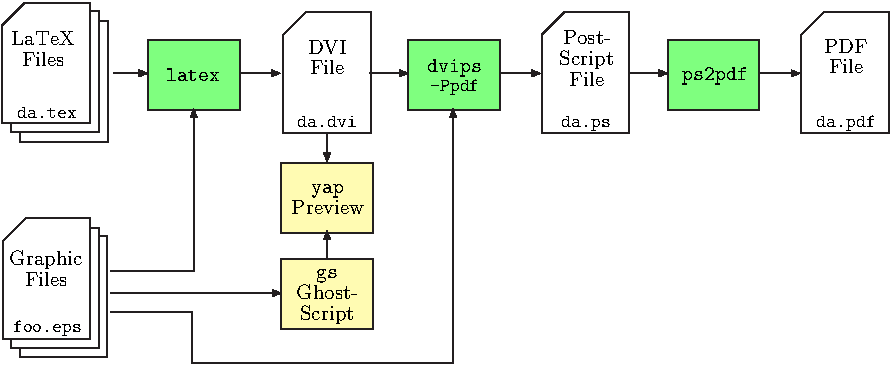
\includegraphics[width=1.0\textwidth]{workflow-cm}
\caption{Erzeugung von
PDF-Doku\-men\-ten im DVI-PS-Workflow. EPS-Grafiken werden erst bei der
Erzeugung der PS-Datei eingebunden. 
Anmerkung: Die abgebildete Vektorgrafik wurde mit \emph{Freehand} unter
Verwendung der \emph{BaKoMa} TrueType-Schriften erstellt %
(s.\ Abschn.\ \ref{sec:tex-schriften-in-grafiken}).}
\label{fig:latex-pdf-workflow}
\end{figure}

\end{comment}


\section{Drucken}

Vor dem Drucken der Arbeit empfiehlt es sich, einige Dinge zu beachten, um unnötigen Aufwand (und auch Kosten) zu vermeiden.

\subsection{Drucker und Papier}

Die Abschlussarbeit sollte in der Endfassung unbedingt auf einem
qualitativ hochwertigen Laserdrucker ausgedruckt werden, Ausdrucke
mit Tintenstrahldruckern sind \emph{nicht} ausreichend. Auch das
verwendete Papier sollte von guter Qualität (holzfrei) und
üblicher Stärke (mind.\ $80\; {\mathrm g} / {\mathrm m}^2$) sein.
Falls \emph{farbige} Seiten notwendig sind, sollte man diese einzeln%
\footnote{Tip: Mit \emph{Adobe Acrobat} lassen sich sehr einfach einzelne Seiten
des Dokuments für den Farbdruck auswählen und zusammenstellen.}
auf einem Farb-Laserdrucker ausdrucken und dem Dokument beifügen.

Übrigens sollten \emph{alle} abzugebenden Exemplare \textbf{gedruckt} (und nicht kopiert) werden! Die Kosten für den Druck
sind heute nicht höher als die für Kopien, der
Qualitätsunterschied ist jedoch -- \va\ bei Bildern und Grafiken
-- meist deutlich.


\subsection{Druckgröße}

Zunächst sollte sichergestellt werden, dass die in der fertigen PDF-Datei eingestellte
Papiergröße tatsächlich \textbf{A4} ist! Das geht \zB\ mit \emph{Adobe Acrobat}
oder \emph{SumatraPDF}
über \texttt{File} $\rightarrow$ \texttt{Properties},
wo die Papiergröße des Dokuments angezeigt wird:
\begin{center}
\textbf{Richtig:} A4 = $8{,}27 \times 11{,}69$ in \bzw\ $21{,}0 \times 29{,}7$ cm.
\end{center}
Falls das nicht stimmt, ist vermutlich irgendwo im Workflow versehentlich \textbf{Letter} 
als Papierformat eingestellt, %, häufig ist \emph{Adobe Distiller} "schuld".


Ein häufiger und leicht zu übersehender Fehler beim Ausdrucken von
PDF-Doku\-menten wird durch die versehentliche Einstellung der
Option "Fit to page" im Druckmenü verursacht, wobei die Seiten
meist zu klein ausgedruckt werden. Überprüfen Sie daher die Größe
des Ausdrucks anhand der eingestellten Zeilenlänge oder mithilfe
einer Messgrafik, wie am Ende dieses Dokuments gezeigt.
Sicherheitshalber sollte diese Messgrafik bis zur
Fertigstellung der Arbeit beibehalten und die entsprechende
Seite erst ganz am Schluss zu entfernt werden.
Wenn, wie häufig der Fall, einzelne Seiten getrennt in Farbe gedruckt 
werden, so sollten natürlich auch diese genau auf die Einhaltung der Druckgröße 
kontrolliert werden!




\section{Binden}

Die Endfassung der Abschlussarbeit%
\footnote{Für \textbf{Bachelorarbeiten} genügt, je nach Vorgaben des Studiengangs, meist eine einfache Bindung (Copyshop oder Bibliothek).}
ist in fest gebundener Form
einzureichen.%
\footnote{An der Fakultät Hagenberg ist bei Masterarbeiten zumindest eines der
Exemplare \emph{ungebunden} abzugeben -- dieses wird später von einem
Buchbinder in einheitlicher Form gebunden und verbleibt
danach in der Bibliothek. Datenträger sind bei diesem Exemplar lose 
und \emph{ohne} Aufkleber (jedoch beschriftet) beizulegen.}
Dabei ist eine Bindung zu
verwenden, die das Ausfallen von einzelnen Seiten nachhaltig
verhindert, \zB durch eine traditionelle Rückenbindung
(Buchbinder) oder durch handelsübliche Klammerungen aus Kunststoff
oder Metall. Eine einfache Leimbindung ohne Verstärkung ist
jedenfalls \emph{nicht} ausreichend.


Falls man -- was sehr zu empfehlen ist -- die Arbeit bei einem
professionellen Buchbinder durchführen lässt, sollte man auch auf
die Prägung am Buchrücken achten, die kaum zusätzliche Kosten
verursacht. Üblich ist dabei die Angabe des Familiennamens des
Autors und des Titels der Arbeit. Ist der Titel der Arbeit zu
lang, muss man notfalls eine gekürzte  Version angeben, wie \zB:
%
\begin{center}
\setlength{\fboxsep}{3mm}
\fbox{
\textsc{Schlaumeier}
\textperiodcentered\ \textsc{Part.\ Lösungen zur allg.\ Problematik}}
\end{center}
%



\section{Elektronische Datenträger (CD-R, DVD, USB-Stick)}
Speziell bei Arbeiten im Bereich der Informationstechnik (aber
nicht nur dort) fallen fast immer Informationen an, wie Programme,
Daten, Grafiken, Kopien von Internetseiten \usw, die für eine
spätere Verwendung elektronisch verfügbar sein sollten.
Vernünftigerweise wird man diese Daten während der Arbeit bereits
gezielt sammeln und der fertigen Arbeit auf einer CD-ROM, DVD oder
einem USB-Stick beilegen. Es ist außerdem sinnvoll -- schon allein
aus Gründen der elektronischen Archivierbarkeit -- die eigene Arbeit
selbst als PDF-Datei beizulegen.%
\footnote{Auch Bilder und Grafiken könnten in elektronischer Form nützlich
sein, die \latex- oder Word-Dateien sind hingegen überflüssig.}


Falls ein elektronischer Datenträger (CD-ROM, DVD, USB-Stick) beigelegt
wird, sollte auf folgende Dinge geachtet werden:
%
\begin{enumerate}
\item Jedem abzugebenden Exemplar muss eine identische Kopie des
Datenträgers beiliegen. %
\item Verwenden Sie qualitativ hochwertige Rohlinge und überprüfen
Sie nach der Fertigstellung die tatsächlich gespeicherten Inhalte
des Datenträgers! %
\item Der Datenträger sollte in eine im hinteren Umschlag
eingeklebte Hülle eingefügt sein und sollte so zu entnehmen sein,
dass die Hülle dabei \emph{nicht} zerstört wird (die
meisten Buchbinder haben geeignete Hüllen parat). %
\item Der Datenträger muss so beschriftet sein, dass er der
Abschlussarbeit eindeutig zuzuordnen ist, am Besten durch ein
gedrucktes Label%
\footnote{Nicht beim lose abgegebenen Bibliotheksexemplar --
dieses erhält ein standardisiertes Label durch die Bibliothek.} %
oder sonst durch \emph{saubere}
Beschriftung mit
der Hand und einem feinen, wasserfesten Stift. %
\item Nützlich ist auch ein (grobes) Verzeichnis der Inhalte des
Datenträgers (wie exemplarisch in Anhang \ref{app:cdrom}).
\end{enumerate}

\chapter[Schlussbemerkungen]%
        {Schlussbemerkungen%
        \protect\footnote{Diese Anmerkung dient nur dazu, die (in seltenen Fällen sinnvolle)
				Verwendung von Fußnoten bei Überschriften zu demonstrieren.}}%
\label{cha:Schluss}

An dieser Stelle sollte eine Zusammenfassung der Abschlussarbeit
stehen, in der auch auf den Entstehungsprozess, persönliche
Erfahrungen, Probleme bei der Durchführung,
Verbesserungsmöglichkeiten, mögliche %
Erweiterungen \usw\ eingegangen werden kann. War das Thema richtig
gewählt, was wurde konkret erreicht, welche Punkte blieben offen
und wie könnte von hier aus weitergearbeitet werden?


\section{Lesen und lesen lassen}

Wenn die Arbeit fertig ist, sollten Sie diese zunächst selbst nochmals vollständig und sorgfältig durchlesen, auch wenn man vielleicht das mühsam entstandene Produkt längst nicht mehr sehen möchte. Zusätzlich ist sehr zu empfehlen, auch einer weiteren Person diese Arbeit anzutun -- man wird erstaunt sein, wie viele Fehler man selbst überlesen hat. 



\section{Checkliste}

Abschließend noch eine kurze Liste der wichtigsten Punkte, an denen erfahrungsgemäß die häufigsten Fehler auftreten (Tab.\ \ref{tab:checkliste}).


\begin{table}
\caption{Checkliste. Diese Punkte bilden auch die Grundlage der routine\-mäßigen Formbegutachtung in Hagenberg.}
\label{tab:checkliste}
\centering%
\setlength{\fboxrule}{0.2mm}%
\setlength{\fboxsep}{2mm}%
\fbox{%
\begin{minipage}{0.95\textwidth}
\begin{itemize}
\item[$\Box$] \textbf{Titelseite:} 
	Länge des Titels (Zeilenumbrüche), Name, Studiengang, Datum.
\item[$\Box$] \textbf{Erklärung:} 
vollständige Unterschrift.
\item[$\Box$] \textbf{Inhaltsverzeichnis:}
	balancierte Struktur, Tiefe, Länge der Überschriften.
\item[$\Box$] \textbf{Kurzfassung/Abstract:} 
	präzise Zusammenfassung, passende Länge, gleiche Inhalte und Struktur.
\item[$\Box$] \textbf{Überschriften:}
	Länge, Stil, Aussagekraft.
\item[$\Box$] \textbf{Typographie:}
	sauberes Schriftbild, keine "manuellen" Abstände zwischen Absätzen oder Einrückungen, 
	keine überlangen Zeilen, Hervorhebungen, Schriftgröße, Platzierung von Fußnoten.
\item[$\Box$] \textbf{Sprache:}
	geschlechtergerechte Formulierungen (kein generisches Maskulinum oder Generalklausel),
	neutraler, sachlicher Stil, keine übermäßigen Anglizismen.
\item[$\Box$] \textbf{Interpunktion:} 
	Binde- und Gedankenstriche richtig gesetzt, Abstände nach Punkten (\va\ nach Abkürzungen),
	korrekte (vordere/hintere) Hochkommas.
\item[$\Box$] \textbf{Abbildungen:}
	Qualität der Grafiken und Bilder, Schriftgröße und -typ in Abbildungen, 
	Platzierung von Abbildungen und Tabellen, Captions. Sind \emph{alle} Abbildungen 
	(und Tabellen) im Text referenziert?
\item[$\Box$] \textbf{Gleichungen/Formeln:}
	mathem.\ Elemente auch im Fließtext richtig gesetzt, explizite Gleichungen
	richtig verwendet, Verwendung von mathem.\ Symbolen.
\item[$\Box$] \textbf{Quellenangaben:}
	Zitate richtig referenziert, Seiten- oder Kapitelangaben.
\item[$\Box$] \textbf{Literaturverzeichnis:}
	Art der Publikation muss in jedem Fall klar sein, konsistente und vollständige Einträge, 
	Online-Quellen (URLs)	sauber angeführt.
\item[$\Box$] \textbf{Sonstiges:} 
	ungültige Querverweise (\textbf{??}), Anhang, Papiergröße der PDF-Datei 
	(A4 = $8.27 \times 11.69$ Zoll), Druckgröße und -qualität.
\end{itemize}
\end{minipage}%
}
\end{table}




%%%----------------------------------------------------------
\appendix                                            % Anhang 
%%%----------------------------------------------------------

\chapter{Technische Informationen}
\label{app:TechnischeInfos}

\newcommand*{\checkbox}{{\fboxsep 1pt%
\framebox[1.30\height]{\vphantom{M}\checkmark}}}

\section{Aktuelle Dateiversionen}

\begin{center}
\begin{tabular}{|l|l|}
\hline
Datum & Datei \\
\hline\hline
\hgbDate       & \texttt{hgb.sty} \\
\hline
\end{tabular}
\end{center}


\section{Details zur aktuellen Version}


Das ist eine völlig überarbeitete Version der DA/BA-Vorlage, die
\mbox{UTF-8} kodierte Dateien vorsieht und ausschließlich im PDF-Modus arbeitet.
Der "klassische" DVI-PS-PDF-Modus wird somit nicht mehr unterstützt!

\subsection{Allgemeine technische Voraussetzungen}

Eine aktuelle \latex-Installation mit
\begin{itemize}
		\item \texttt{biber}-Programm (BibTeX-Ersatz, Version $\geq 1.5$),
		\item \texttt{biblatex}-Paket (Version $\geq 2.5$, 2013/01/10),
		\item Latin Modern Schriften (Paket \texttt{lmodern}).%
			\footnote{\url{https://www.ctan.org/pkg/lm}, \url{https://tug.org/FontCatalogue/latinmodernroman/}}
\end{itemize}

Darüber hinaus ein Texteditor für \mbox{UTF-8} kodierte (Unicode) Dateien, sowie Software zum Öffnen und Betrachten von PDF-Dateien.


\subsection{Verwendung unter Windows}
\label{sec:VerwendungUnterWindows}

Eine typische Installation unter Windows sieht folgendermaßen aus:
%
\begin{enumerate}
\item \textbf{MikTeX}%
	\footnote{\url{https://miktex.org/} -- \textbf{Achtung:} 
	Generell wird die \textbf{Komplettinstallation} von MikTeX ("Complete MiKTeX") empfohlen, 
	da diese bereits alle notwendigen Zusatzpakete und Schriftdateien enthält. Hierzu wird der
	MikTeX Net Installer (im Gegensatz zum Basic Installer) benötigt.
	Bei der Installation ist darauf zu achten, 
	dass die automatische Installation erforderlicher Packages 
	durch "\emph{Install missing packages on-the-fly: = Yes}" ermöglicht wird (NICHT "\emph{Ask me first}")!
	Außerdem ist zu empfehlen, unmittelbar nach der Installation von MikTeX sowie in weiterer Folge regelmäßig
	mit dem Programm \texttt{MikTeX Console} ein Update der installierten Pakete durchzuführen.}
	(\latex-Basisumgebung),
\item \textbf{TeXstudio}%
	\footnote{\url{https://www.texstudio.org/}}
	(Editor, unterstützt UTF-8 und beinhaltet einen integrierten PDF-Viewer).
\end{enumerate}

Alternative Editoren und PDF-Viewer:
%
\begin{enumerate}
	\item TeXnicCenter,%
	\footnote{\url{https://www.texniccenter.org/}}
	\item Texmaker,%
	\footnote{\url{https://www.xm1math.net/texmaker/}}
	\item Lyx,%
	\footnote{\url{https://www.lyx.org/}}
	\item TeXworks,%
	\footnote{\url{https://www.tug.org/texworks/}}
	\item WinEdt,%
	\footnote{\url{https://www.winedt.com/}}
	\item Sumatra PDF (\latex-freundlicher PDF-Viewer).%
	\footnote{\url{https://www.sumatrapdfreader.org/}}
\end{enumerate}

\subsection{Verwendung unter Mac~OS}

Für Mac~OS empfiehlt sich die folgende Konfiguration:
%
\begin{enumerate}
\item 
	\textbf{MacTex}%
	\footnote{\url{https://tug.org/mactex/} -- \textbf{Achtung:} Aktuelle MacTeX-Distributionen verlangen in
		der Regel eine weitgehend aktuelle Version von Mac~OS. Auf älteren Betriebssystemen kann alternativ
		TeXLive mit einem speziellen Installationsscript installiert werden.
		Um die Pakete der \LaTeX-Distribution aktuell zu halten, sollte regelmäßig das \texttt{TeX Live Utility}
		ausgeführt werden.}
	(\latex-Basisumgebung),
\item \textbf{TeXstudio}%
	(Editor, unterstützt UTF-8 und beinhaltet einen integrierten PDF-Viewer).
\end{enumerate}

Alternative Editoren und PDF-Viewer:
%
\begin{enumerate}
	\item Texmaker,%
	\item Lyx,%
	\item TeXworks,%
	\item Skim (\latex-freundlicher PDF-Viewer).%
	\footnote{\url{https://skim-app.sourceforge.io/}}
\end{enumerate}

\subsection{Verwendung unter Linux}

Unter Linux kann folgendes Setup zum Einsatz kommen:
%
\begin{enumerate}
	\item 
	\textbf{TeX Live}%
	\footnote{\url{https://tug.org/texlive/} -- Eine Installation unter Linux erfolgt -- abhängig von der verwendeten
	Distribution -- am einfachsten mit Hilfe des jeweiligen Paketverwaltungssystems (\zB \texttt{apt-get}).}
	(\latex-Basisumgebung),
	\item \textbf{TeXstudio}%
	(Editor, unterstützt UTF-8 und beinhaltet einen integrierten PDF-Viewer).
\end{enumerate}

Alternative Editoren und PDF-Viewer:
%
\begin{enumerate}
	\item Texmaker,%
	\item Lyx,%
	\item TeXworks,%
	\item qpdfview (\latex-freundlicher PDF-Viewer).%
	\footnote{\url{https://launchpad.net/qpdfview}}
\end{enumerate}

\subsection{Verwendung von Online-Editoren}

Neben einer lokalen \latex-Installation mit Editor gibt es mittlerweile auch Online-Editoren, die das Arbeiten mit \latex-Dokumenten
im Browser ermöglichen. Die \latex-Basisumgebung ist dabei auf den Servern des Dienstes installiert, Dokumente können im Editor neu
erstellt oder auch bestehende Vorlagen (wie etwa dieses Dokument) hochgeladen und weiter bearbeitet werden. Die meisten Plattformen
ermöglichen darüber hinaus ein kollaboratives Arbeiten an einem Dokument.

Der bekannteste und mit dieser Vorlage getestete Editor ist \emph{Overleaf}\footnote{\url{https://www.overleaf.com/}}. Um schnell
Vorlagendokumente aus dem \texttt{hagenberg-thesis} Paket zu importieren, können die Import-Links in der Readme zum Repository
dieser Vorlage\footnote{\url{https://github.com/Digital-Media/HagenbergThesis}} verwendet werden.

Alternativ existieren noch weitere Online-Editoren:
%
\begin{enumerate}
	\item Papeeria,%
	\footnote{\url{https://papeeria.com/}}
	\item CoCalc.%
	\footnote{\url{https://cocalc.com/}}
\end{enumerate}
	% Technische Ergänzungen
\chapter{Inhalt der CD-ROM/DVD}
\label{app:cdrom}

\paragraph{Format:} 
		CD-ROM, Single Layer, ISO9660-Format%
\footnote{Verwenden Sie möglichst ein Standardformat, bei DVDs natürlich
eine entsprechende andere Spezifikation.}


\section{PDF-Dateien}
\begin{FileList}{/}
%\fitem{_DaBa.dvi} Gesamtdokument (DVI-File, ohne Grafiken)
\fitem{_thesis_DE.pdf} Master- oder Bachelorarbeit mit Instruktionen (Gesamtdokument)
\fitem{_praktikum.pdf} Praktikumsbericht (verkürzte Version der Bachelorarbeit) %
\end{FileList}


\section{\latex-Dateien}

\textbf{Achtung:} Die folgende Auflistung soll nur den Gebrauch dieser Vorlage erleichtern. Es ist bei einer Master- oder Bachelorarbeit \ia\ \emph{nicht} notwendig, die zugehörigen \latex-Dateien aufzulisten (wohl aber projektbezogene Dateien, Ergebnisse, Bilder, Kopien von Online-Literatur etc.)!

\begin{FileList}{/}
\fitem{_thesis_DE.tex} Master-/Bachelorarbeit (Hauptdokument) %
\fitem{_praktikum.tex} Praktikumsbericht (verkürzte Version der Bachelorarbeit) %
\fitem{references.bib} Literatur-Datenbank (BibTeX-File)
\end{FileList}

\begin{FileList}{/thesis_DE/front}
\fitem{vorwort.tex} Vorwort %
\fitem{kurzfassung.tex} Kurzfassung %
\fitem{abstract.tex} Abstract %
\end{FileList}

\begin{FileList}{/thesis_DE/chapters}
\fitem{einleitung.tex} Kapitel 1 %
\fitem{diplomschrift.tex} Kapitel 2 %
\fitem{latex.tex} Kapitel 3
\fitem{abbildungen.tex} Kapitel 4 %
\fitem{formeln.tex} Kapitel 5 %
\fitem{literatur.tex} Kapitel 6 %
\fitem{drucken.tex} Kapitel 7 %
\fitem{word.tex} Kapitel 8 %
\fitem{schluss.tex} Kapitel 9 %
\end{FileList}

\begin{FileList}{/thesis_DE/back}
\fitem{anhang_a.tex} Anhang A (Source Code) %
\fitem{anhang_b.tex} Anhang B (Inhalt CD-ROM) %
\fitem{anhang_c.tex} Anhang C (Liste der Änderungen) %
\fitem{anhang_d.tex} Anhang D (LaTeX-Quellcode) %
\fitem{messbox.tex} Messbox zur Druckkontrolle %
\end{FileList}

\section{Style/Class-Dateien}

\begin{FileList}{/}
\fitem{hgbthesis.cls} LaTeX Class-Datei für Master- und Bachelorarbeiten
\fitem{hgb.sty} LaTeX Style-Datei für alle Hagenberg-Dokumente
\fitem{hgbabbrev.sty} LaTeX Style-Datei mit Abkürzungs-Makros
\fitem{hgbbib.sty} LaTeX Style-Datei mit Bibiographie-Einstellungen
\fitem{hgbheadings.sty} LaTeX Style-Datei für Überschriften
\fitem{hgblistings.sty} LaTeX Style-Datei für Code-Umgebungen
\end{FileList}


\section{Sonstiges}

\begin{FileList}{/images}
\fitem{*.ai} Original Adobe Illustrator-Dateien %
\fitem{*.fh11} Original Macromedia Freehand-Dateien %
\fitem{*.jpg, *.png} Original Rasterbilder %
\end{FileList}
	% Inhalt der CD-ROM/DVD
\chapter{Fragebogen}
\label{app:Fragebogen}


Dieser Abschnitt demonstriert -- als Beispiel -- die Einbindung eines externen PDF-Dokuments
in das eigene \latex-Manuskript.
Dieses Problem stellt sich relativ häufig im Zusammenhang mit Fragebögen, die
man für seine Arbeit erstellt und/oder verwendet hat, daher ist genau dieser Fall hier gezeigt.%
\footnote{Mit einem schönen Fragebogen des OÖ Energiesparverbands (\url{https://www.energiesparverband.at/}).}
Wichtig ist dabei, dass die \emph{Seitenformatierung} des Dokuments intakt bleibt 
und die fortlaufende \emph{Seitennummerierung} die eingefügten Fremdseiten korrekt berücksichtigt.

\section{Das \texttt{pdfpages}-Paket}

Das \latex-Paket \texttt{pdfpages}%
\footnote{\url{https://ctan.org/pkg/pdfpages}}
ist dafür die (zurzeit) einzige Wahl und es wird mit 
%
\begin{LaTeXCode}[numbers=none]
\RequirePackage{pdfpages}
\end{LaTeXCode}
%
in der Datei \nolinkurl{hgb.sty} automatisch geladen.
Das eingebundene PDF-Dokument (der zweiseitige Frage\-bogen) liegt in
\nolinkurl{images/fragebogen.pdf}.
Um nachfolgend alle (2) Seiten der PDF-Datei in das aktuelle Dokument einzubinden,
verwenden wir die Anweisung  
%
\begin{LaTeXCode}[numbers=none]
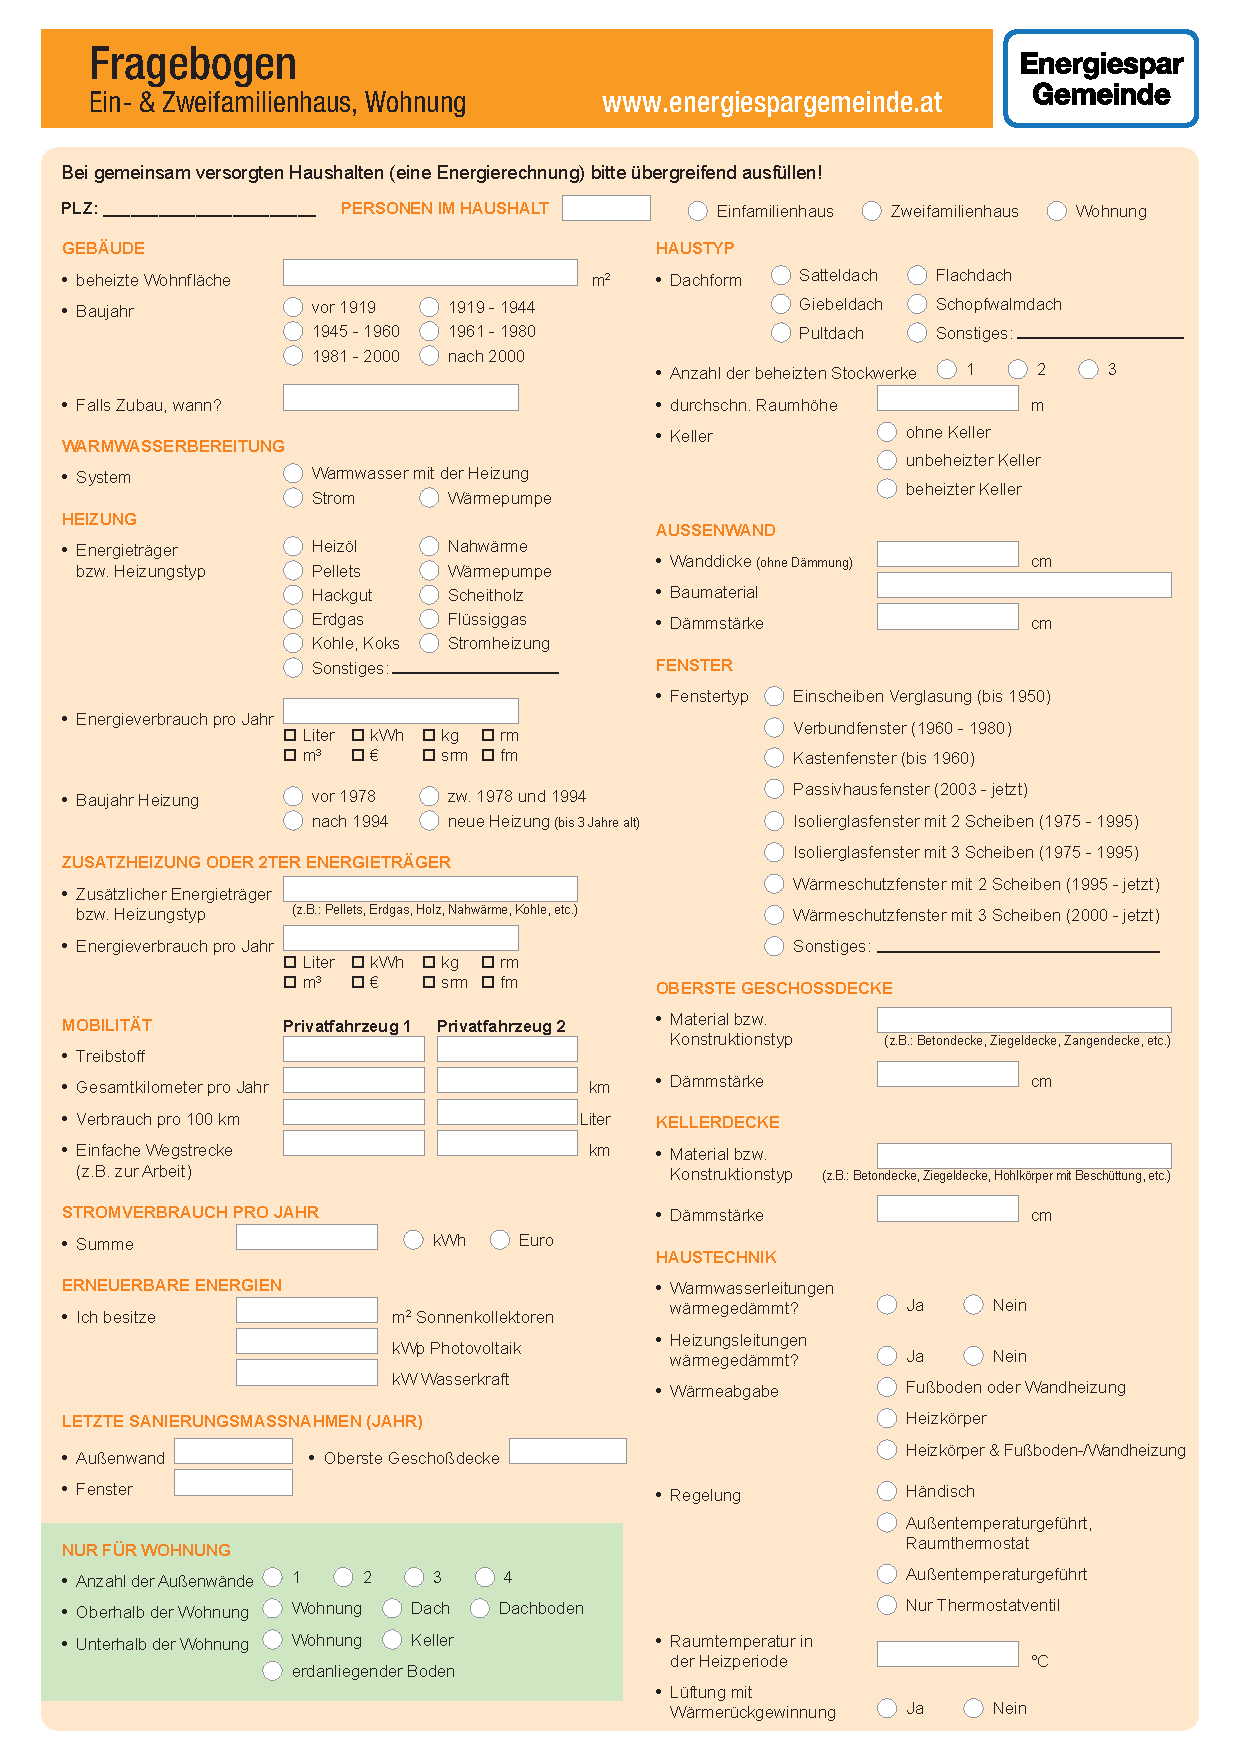
\includepdf[pages=1-,width=\textwidth,frame=true,pagecommand={}]{images/fragebogen}
\end{LaTeXCode}
%
Die eingebundenen Seiten werden durch \verb!width=\textwidth! automatisch auf die Textbreite
des \latex-Dokuments skaliert und durch \verb!frame=true! mit einer Umrandung versehen.

Dieses Beispiel geht davon aus, dass das externe PDF-Dokument im A4-Seitenformat ist.
Bei anderen Formaten muss man die Skalierung möglicherweise "händisch" einstellen,
falls die Seiten zu hoch werden (\zB\ mit \verb!width=0.9\textwidth!).

Wichtig ist auch, dass bei dem externen PDF-Dokument alle verwendeten \emph{Schriften}
(Fonts) korrekt und vollständig \emph{eingebettet} sind, da ansonsten das von \latex erzeugte 
PDF-Dokument nicht unabhängig von der Systemumgebung ist!


\section{Verweise auf eingebundene PDF-Seiten}

Möchte man im Text auf bestimmte PDF-Seiten verweisen,
so ist es am Einfachsten, die Seiten einzeln zu importieren und jeweils
mit einem \emph{Label} zu versehen, wie in diesem Beispiel:
%
\begin{LaTeXCode}[numbers=none]
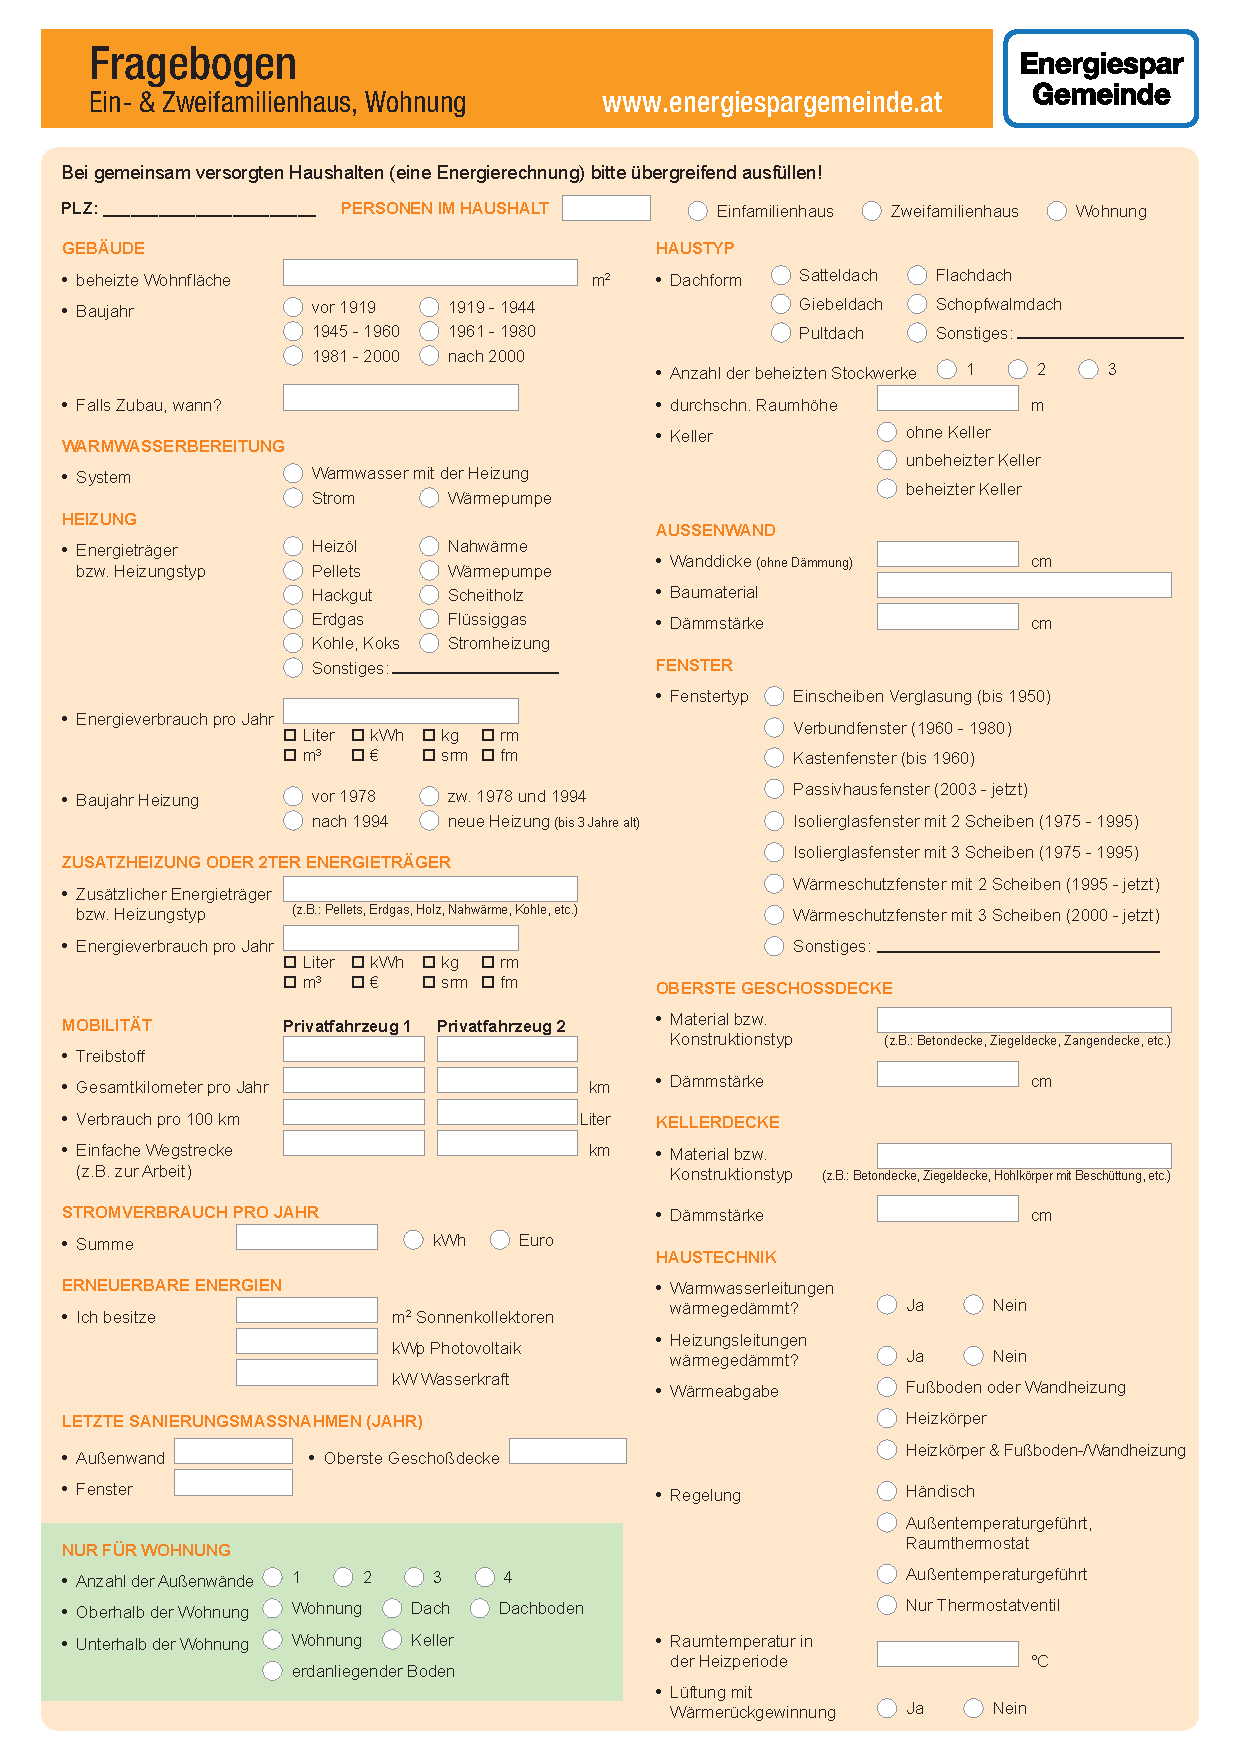
\includepdf[pages=1,width=\textwidth,frame=true,pagecommand={\label{PDF1}}]{images/fragebogen}
\includepdf[pages=2,width=\textwidth,frame=true,pagecommand={\label{PDF2}}]{images/fragebogen}
\end{LaTeXCode}
%
In diesem Fall könnte man beispielsweise mit \verb!\pageref{PDF2}!
die aktuelle Seitennummer der 2.\ Seite des eingebundenen PDF-Dokuments 
angeben.

Viele weitere Möglichkeiten (\zB\ die Angabe von Seitenintervallen) findet man
in der ausführlichen Dokumentation zum \texttt{pdfpages}-Paket.



% Und hiermit werden die PDF-Seiten tatsächlich eingebunden:
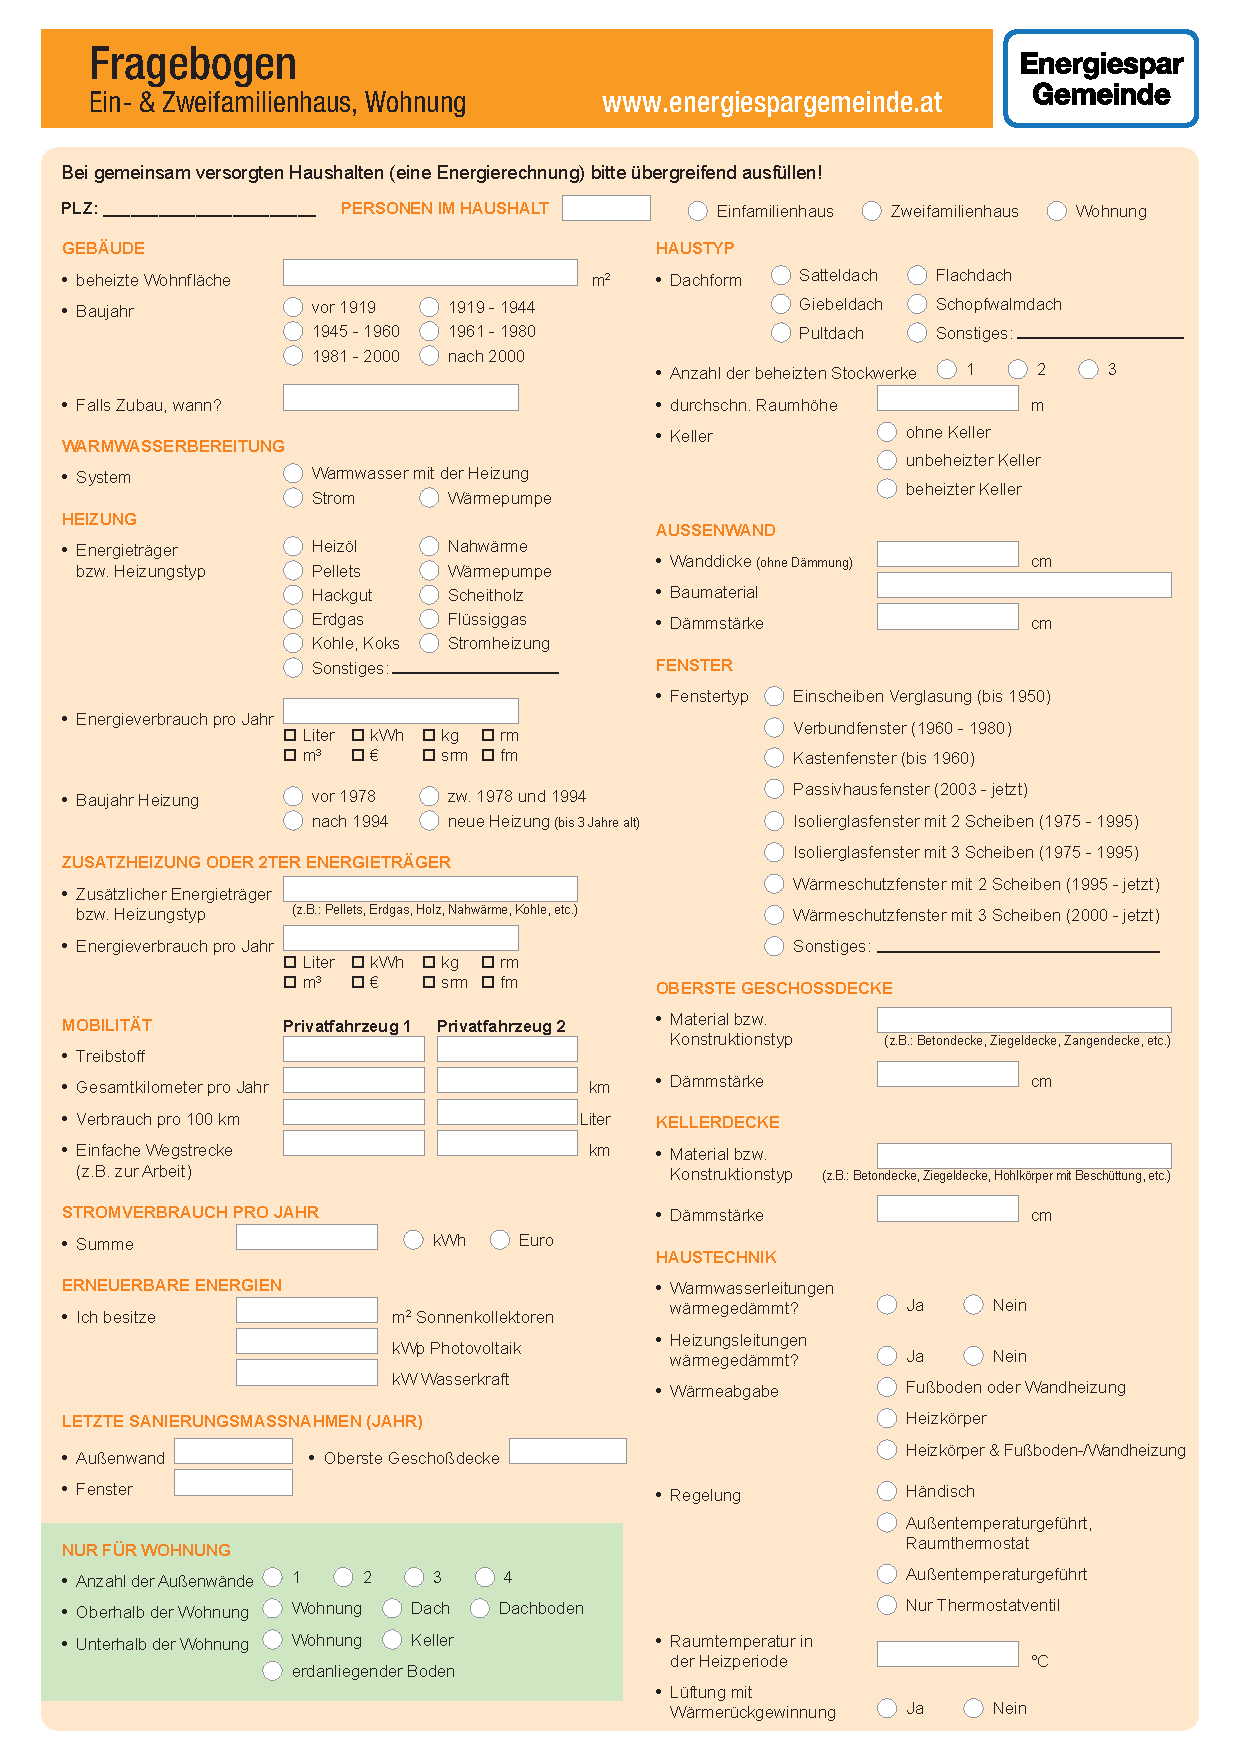
\includepdf[pages=1-,width=\textwidth,frame=true,pagecommand={}]{images/fragebogen}



	% Chronologische Liste der Änderungen
\chapter{\latex-Quellcode}
\label{app:Quellcode}

	% Quelltext dieses Dokuments

%%%----------------------------------------------------------
\MakeBibliography                        % Quellenverzeichnis
%%%----------------------------------------------------------

%%% Messbox zur Druckkontrolle ------------------------------
\chapter*{Messbox zur Druckkontrolle}



\begin{center}
{\Large --- Druckgröße kontrollieren! ---}

\bigskip

\calibrationbox{100}{50} % Angabe der Breite/Hoehe in mm

\bigskip

{\Large --- Diese Seite nach dem Druck entfernen! ---}

\end{center}



%%%----------------------------------------------------------
\end{document}
%%%----------------------------------------------------------